
\documentclass[12pt,a4paper]{report}

% ---------- Encoding & Language ----------
% The report is written in English, but a small number of Vietnamese strings are
% unavoidable: source titles in references.bib, province names used by the fee
% module, and the OCR error examples in Chapter 5 (whose whole point is a
% diacritic error). T1 cannot represent those characters, so T5 (vntex) is
% loaded alongside it for pdfLaTeX. If the compiler is XeLaTeX or LuaLaTeX,
% fontspec is used instead. Everything else is unchanged from the template.
\usepackage{iftex}
% ---------- Times New Roman, everywhere ----------
% Text/sans/mono all use TeX Gyre Termes, the metric-compatible Times New Roman
% clone shipped with TeX Live; unlike newtx/T1 it also covers the Vietnamese
% characters in the reference list and the OCR examples. mathptmx is loaded
% BEFORE fontspec so that formulas are set in Times too, while \setmainfont
% still wins for running text. Requires XeLaTeX.
\ifPDFTeX
  \usepackage[utf8]{inputenc}
  \usepackage[T1,T5]{fontenc}
  \AtBeginDocument{\typeout{^^J*** Compile with XeLaTeX to get Times New Roman. ***^^J}}
\else
  \usepackage{mathptmx}          % Times math
  \usepackage{fontspec}
  \setmainfont{TeX Gyre Termes}
  \setsansfont{TeX Gyre Termes}
  \setmonofont{TeX Gyre Termes}  % \texttt{} in Times as well, not a typewriter face
\fi
\usepackage[english]{babel}
\addto\captionsenglish{\renewcommand{\contentsname}{Table of Contents}}

% ---------- Page Geometry & Spacing ----------
\usepackage{geometry}
\geometry{margin=1in}
\usepackage{setspace}
\onehalfspacing
% Uniform inter-word spacing. By default LaTeX inserts a wider space after a
% sentence-ending period, which at 12pt with 1.5 line spacing reads as an
% uneven gap in the middle of a line.
\frenchspacing

% ---------- Figures, Tables, Math ----------
\usepackage{graphicx}
\usepackage{booktabs}
\usepackage{tabularx}
\usepackage{longtable}
\usepackage{float}
\usepackage{amsmath, amssymb}
\usepackage{array}
\usepackage{enumitem}
\usepackage{ragged2e}
\usepackage{algorithm}
\usepackage{algpseudocode} % If using algorithmic pseudocode syntax

\setlist[itemize]{nosep,leftmargin=*}    % compact lists inside cells
\newcolumntype{R}[1]{>{\raggedright\arraybackslash}p{#1}} % ragged-right wrapped column
% Plain \raggedright (infinite rightskip) rather than ragged2e's \RaggedRight:
% with hyphenation disabled globally, the finite stretch of \RaggedRight makes
% every short cell report "Underfull \\hbox (badness 10000)".
\setlength{\arrayrulewidth}{0.4pt}       % border thickness (adjust if needed)
\renewcommand{\arraystretch}{1.05}       % row height (optional)

% ---------- Lists & Formatting ----------
\usepackage{enumitem}
\setlist{leftmargin=2em}
\usepackage{xurl} % allow long URLs in the bibliography to break across lines
\usepackage{hyperref}
\hypersetup{
    colorlinks=true,
    linkcolor=blue,
    citecolor=blue,
    urlcolor=blue,
    pdfauthor={Hoang Quoc Dung, Do Thanh Hung, Le Huy Anh, Bui Nhat Minh},
    pdftitle={Designing an AI-Integrated Automation System for Post Offices},
}

% ---------- Typography & Hyphenation ----------
% Font expansion is a pdfTeX-only feature; XeLaTeX aborts on it.
\ifPDFTeX
  \usepackage[protrusion=true,expansion=true]{microtype}
  \microtypesetup{verbose=silent}
\else
  \usepackage[protrusion=true,expansion=false]{microtype}
\fi
% Hyphenation is left ON. The template's \usepackage[none]{hyphenat} plus \sloppy
% is what produced the very wide, uneven word gaps in justified paragraphs:
% with no legal break point inside a long word, TeX can only stretch the spaces.
% A small \emergencystretch handles the few remaining hard lines without
% resorting to \sloppy.
\setlength{\emergencystretch}{2em}
\hyphenpenalty=1000
\tolerance=1500

% ---------- Heading depth ----------
% Numbering and the table of contents stop at section level (1, 1.1, 1.2, ...).
% Subsections are still typeset as unnumbered headings. Set both counters to 2
% to restore the 1.1.1 numbering used by the original template.
\setcounter{secnumdepth}{1}
\setcounter{tocdepth}{1}

% ---------- Custom Commands ----------
\newcommand{\todo}[1]{\textbf{\color{red}[TODO: #1]}}

% ---------- frame of title page ----------
\usepackage{tikz}
\newcommand{\pageframe}{%
  \begin{tikzpicture}[remember picture,overlay]
    \draw[line width=0.8pt]
      ([xshift=1cm,yshift=-1cm]current page.north west)
      rectangle
      ([xshift=-1cm,yshift=1cm]current page.south east);
  \end{tikzpicture}%
  \begin{tikzpicture}[remember picture,overlay]
    \draw[line width=0.8pt]
      ([xshift=1.1cm,yshift=-1.1cm]current page.north west)
      rectangle
      ([xshift=-1.1cm,yshift=1.1cm]current page.south east);
  \end{tikzpicture}%
}

\begin{document}

\begin{titlepage}
    \pageframe 
    \begin{center}
        \vspace*{1.5cm} 
        
        % FPTU Logo
        
\includegraphics[width=0.62\linewidth]{Images/fptu_logo.png}

        \vspace*{1.2cm}
        
        % Adjusted title size to fit in one page
        \Large
        \textbf{Designing an AI-Integrated Automation System\\[0.35em] for Post Offices}
 
        \vspace{0.2cm}
        \vfill
        \begin{table}[H]
        \large
        \centering
        \begin{tabular}{rl}
        Team members: & HE181505 - Hoang Quoc Dung \\
                      & HE186333 - Do Thanh Hung  \\
                      & HE187191 - Le Huy Anh \\
                      & HE180948 - Bui Nhat Minh   \\
        Supervisor:      & M.Eng. Nguyen Thi Hoang Yen      
        \end{tabular}
        \end{table}
        \Large

        \vspace{0.25cm}
        \vfill
        \Large
        Bachelor of Artificial Intelligence\\
        FPT University - August 2026\\
    \end{center}
\end{titlepage}


\pagenumbering{roman}
\clearpage\phantomsection\addcontentsline{toc}{chapter}{Acknowledgements}
\chapter*{Acknowledgements}

We would like to express our deepest gratitude to our supervisor, M.Eng. Nguyen Thi Hoang Yen, whose guidance and constructive feedback steered this project at every stage and pushed us to meet a standard of rigor we could not have reached alone.

We are also sincerely grateful to the staff at the post office who took the time to share real operational data and handwritten shipping forms with us. Their cooperation gave the project a genuine, practical foundation that no simulated dataset could have provided.

In addition, we wish to thank the lecturers of FPT University, particularly those from the Artificial Intelligence specialization, for the solid academic training and hands-on experience that made this work possible.

Finally, we are deeply thankful to our families and friends, whose patience, encouragement, and quiet support carried us through to the completion of this project.

\clearpage\phantomsection\addcontentsline{toc}{chapter}{Abstract}
\chapter*{Abstract}
\normalsize

Postal item acceptance at the counter currently depends on many manual operations, such as entering customer information, weighing, measuring dimensions and calculating the shipping fee. This makes a transaction take about 6--8 minutes and can lead to data-entry errors. The project therefore builds a system that combines artificial intelligence with low-cost sensors in order to automate part of this workflow.

The system supports item classification, information extraction, dimension measurement, volume estimation and fee calculation. A You Only Look Once version 11 nano model classifies parcels and envelopes and detects the information region on parcels. EasyOCR detects the text regions and a fine-tuned Transformer-based Optical Character Recognition model recognizes Vietnamese handwriting. Parcel dimensions are determined by one of two methods: two webcams combined with the same detector and Canny edge detection, or three ultrasonic sensors connected to an ESP32 microcontroller together with a temperature sensor. Development and evaluation used 439 postal item images collected by the team, 60,247 Vietnamese handwriting samples, 9,216 parcel images and 26,768 hand images annotated with keypoints.

The results show that the item classification model and the information region detection model reach a mean average precision at an intersection over union threshold of 0.50 of 99.50\% and 97.90\% respectively. After fine-tuning, the recognition model achieves a character error rate of 5.39\% and a word error rate of 14.99\%. With the webcam method, the volume errors on three test samples are 0.31\%, 0.19\% and 1.02\%. With the ultrasonic method, the mean absolute error of the three sensors lies between 0.9016 and 1.7445 centimetres. The fee calculation module also matches manual computation in every test case carried out. Overall, combining low-cost components to support postal item acceptance is feasible, but the system still needs to be evaluated in a real post office environment before any conclusion can be drawn about transaction time or manual data entry.

\vspace{0.5cm}
\noindent\textbf{Keywords:} Postal item acceptance; handwriting recognition; object detection; dimension measurement; shipping fee calculation


\clearpage\phantomsection\addcontentsline{toc}{chapter}{Table of Contents}
\tableofcontents
\clearpage
\phantomsection\addcontentsline{toc}{chapter}{List of Tables}
\listoftables
\clearpage
\phantomsection\addcontentsline{toc}{chapter}{List of Figures}
\listoffigures
\clearpage
\clearpage\phantomsection\addcontentsline{toc}{chapter}{List of Abbreviations and Acronyms}
\chapter*{List of Abbreviations and Acronyms}

\renewcommand{\arraystretch}{1.25}
\begin{longtable}{|>{\raggedright\arraybackslash}p{3.4cm}|>{\raggedright\arraybackslash}p{10.4cm}|}
\hline
\textbf{Acronym} & \textbf{Definition} \\
\hline
\endfirsthead
\hline
\textbf{Acronym} & \textbf{Definition} \\
\hline
\endhead
\hline
\endfoot
\hline
\endlastfoot

\textbf{2D} & Two-Dimensional \\
\hline
\textbf{3D} & Three-Dimensional \\
\hline
\textbf{AI} & Artificial Intelligence \\
\hline
\textbf{AP} & Average Precision, the area under the precision--recall curve for one class \\
\hline
\textbf{API} & Application Programming Interface, as in the Claude API used for structured field extraction \\
\hline
\textbf{BEiT} & Bidirectional Encoder representation from Image Transformers, used to initialize the TrOCR image encoder \\
\hline
\textbf{BiFPN} & Bidirectional Feature Pyramid Network \\
\hline
\textbf{CER} & Character Error Rate \\
\hline
\textbf{CNN} & Convolutional Neural Network \\
\hline
\textbf{CRAFT} & Character Region Awareness for Text Detection, used by EasyOCR to detect text regions \\
\hline
\textbf{CTN001} & Vietnam Post service code using progressive-tier pricing in the fee-calculation module \\
\hline
\textbf{DFL} & Distribution Focal Loss \\
\hline
\textbf{ESP32} & Espressif 32-bit microcontroller with Wi-Fi, used as the central processor of the ultrasonic measurement system \\
\hline
\textbf{ETN} & Group of Vietnam Post service codes using base-tier pricing with additional surcharges \\
\hline
\textbf{ETN001, ETN011, ETN013} & Vietnam Post service codes belonging to the ETN service group \\
\hline
\textbf{F1} & F1 Score, the harmonic mean of precision and recall \\
\hline
\textbf{fp16} & 16-bit floating-point format used for mixed-precision training \\
\hline
\textbf{GND} & Ground, the common electrical reference of the sensor circuit \\
\hline
\textbf{GPIO} & General-Purpose Input/Output, the ESP32 pins connected to the sensors \\
\hline
\textbf{GPU} & Graphics Processing Unit \\
\hline
\textbf{I\textsuperscript{2}C} & Inter-Integrated Circuit, the serial communication bus connecting the \mbox{SHT30-D} to the ESP32 \\
\hline
\textbf{IoU} & Intersection over Union \\
\hline
\textbf{JSON} & JavaScript Object Notation, the structured data format returned by the Claude API and ESP32 \\
\hline
\textbf{MAE} & Mean Absolute Error \\
\hline
\textbf{mAP} & Mean Average Precision \\
\hline
\textbf{mAP@50} & Mean Average Precision at an Intersection over Union threshold of 0.50 \\
\hline
\textbf{mAP@50--95} & Mean Average Precision averaged over Intersection over Union thresholds from 0.50 to 0.95 \\
\hline
\textbf{MAPE} & Mean Absolute Percentage Error \\
\hline
\textbf{MERGE} & Layout-reconstruction step that joins text fragments located on the same row \\
\hline
\textbf{OCR} & Optical Character Recognition \\
\hline
\textbf{OpenCV} & Open Source Computer Vision Library \\
\hline
\textbf{PAIR} & Layout-reconstruction step that pairs a label block with its corresponding value block \\
\hline
\textbf{R-CNN} & Region-based Convolutional Neural Network \\
\hline
\textbf{ResCBAM} & Residual Convolutional Block Attention Module \\
\hline
\textbf{RGB} & Red, Green, Blue, the colour-image format used as input by the text detector \\
\hline
\textbf{RNN} & Recurrent Neural Network \\
\hline
\textbf{RoBERTa} & Robustly Optimized BERT Pretraining Approach, used to initialize the TrOCR text decoder \\
\hline
\textbf{ROI} & Region of Interest, the selected image region used for subsequent processing \\
\hline
\textbf{RTX 3050} & NVIDIA GeForce graphics card with 4 GB of VRAM used for training and inference \\
\hline
\textbf{\mbox{SHT30-D}} & Digital temperature and humidity sensor used to compensate for changes in the speed of sound \\
\hline
\textbf{SPLIT} & Layout-reconstruction step that separates the columns and sender/receiver areas \\
\hline
\textbf{TP.HCM} & Ho Chi Minh City \\
\hline
\textbf{TrOCR} & Transformer-based Optical Character Recognition \\
\hline
\textbf{US1, US2, US3} & Three ultrasonic sensors \\
\hline
\textbf{USB} & Universal Serial Bus \\
\hline
\textbf{VND} & Vietnamese Dong, the currency used in the shipping-fee table \\
\hline
\textbf{VRAM} & Video Random Access Memory \\
\hline
\textbf{WER} & Word Error Rate \\
\hline
\textbf{YOLO} & You Only Look Once \\
\hline
\textbf{YOLO11n} & Nano variant of YOLO11, used for box/envelope detection and information-region detection \\
\hline
\textbf{YOLO26n} & Nano variant of YOLO26, used for person detection \\
\hline
\textbf{YOLO26n-hand} & Fine-tuned YOLO26n variant used for hand-keypoint detection \\
\hline
\textbf{YOLOv12-BiFPN-ResCBAM} & YOLOv12-based architecture integrating BiFPN and ResCBAM \\
\hline

\end{longtable}
\renewcommand{\arraystretch}{1.05}

\clearpage
\pagenumbering{arabic}

\chapter{Introduction}
\label{chap:introduction}

\section{Background and Motivation}
\label{sec:background_motivation}

In the context of the fourth industrial revolution and the rapid progress of artificial intelligence (AI), AI technology is being applied ever more widely across many fields in order to automate processes, raise productivity and reduce dependence on manual operations. In the postal sector, digital transformation does not stop at digitizing records or moving traditional procedures into software; it also aims at automating repetitive steps, standardizing data and improving operational efficiency.

At the item acceptance stage, however, many steps still require the direct involvement of the counter clerk: reading and entering sender and receiver information, weighing the item, measuring its dimensions, entering the data and checking the information before completing the transaction. Based on the team's own observation at the acceptance counter, a typical postal transaction takes about 6--8 minutes. Performing many manual operations may increase waiting time, create pressure during peak hours and introduce the risk of data-entry errors.

Starting from this practical situation, and drawing on the knowledge acquired in the Artificial Intelligence specialization, the team identified this as a problem with strong practical relevance that is amenable to AI-based solutions. The team therefore set out to apply its knowledge of computer vision, image recognition and data processing to build a solution that can help automate the postal acceptance process, in particular information recognition, parcel dimension determination and the computation of the required parameters.

\section{Literature Review}

Recent studies show that computer vision and deep learning are increasingly being applied to the automation of postal item processing. The research directions most directly related to this topic are text recognition, object detection, parcel dimension measurement, and the use of depth information to reconstruct three-dimensional dimensions.

Li et al.~\cite{li2023trocr} proposed TrOCR to address text recognition from images, particularly handwriting. Unlike traditional OCR systems that combine convolutional and recurrent networks, TrOCR uses a Transformer with an image encoder and a text decoder in an end-to-end architecture. The results show that TrOCR performs well on printed text, handwriting and scene text datasets. The advantage of the method is that it exploits pretrained models and can be fine-tuned for different data domains. Even so, the model still needs to be adapted to the linguistic and data characteristics of each application. This matches the present project, in which the team inherits TrOCR and fine-tunes it on Vietnamese handwriting data in order to recognize information on shipping forms.

For dimension measurement, Fernandes et al.~\cite{fernandes2006} studied a method for determining box dimensions from camera images. The method relies on perspective geometry, the box outline, and information from laser beams to infer the real dimensions of the object. The advantage is a clear geometric foundation and the ability to measure automatically from images. However, the use of lasers increases the hardware requirements and makes the system dependent on the measurement configuration. Following this direction, the present project also uses images to determine parcel dimensions, but replaces the laser system with YOLO, region-of-interest extraction and Canny edge detection, and then converts pixel dimensions into real-world units.

Peng et al.~\cite{peng2020} approached box dimension measurement by combining laser triangulation and deep learning. The method exploits the geometric and depth information obtained from a structured light system to determine box features. Compared with methods that use only two-dimensional images, this approach has the advantage of capturing three-dimensional information and can improve dimension measurement. However, the system requires specialized optical devices such as a laser projector, which increases cost and deployment complexity. This study shows that depth information is an effective direction for dimension measurement, but at the same time raises the issue of hardware cost and complexity.

A different direction is presented in the thesis \textit{Applying 3D cameras to product classification by shape and size} \cite{lethai2019}, which uses stereo vision to capture three-dimensional information. Two cameras observe the same object from different angles, and the disparity between corresponding points is then used to estimate depth. The advantage of the method is that three-dimensional spatial information can be obtained without physical contact with the object. However, accuracy depends on camera placement, the distance to the object and the ability to identify corresponding points; occlusion and overlapping objects also cause difficulties for the system. This work is directly related to the multi-camera dimension measurement direction of the project, but the team chose a simpler approach based on two cameras and geometric relations rather than building a complete stereo reconstruction system.

More recently, Tran et al.~\cite{tran2026} proposed an integrated parcel processing system based on YOLOv12-BiFPN-ResCBAM, targeting barcode recognition, dimension measurement and parcel damage detection. The study reflects a shift in the field from solving individual tasks towards building automated systems that integrate multiple functions. The advantage of the method is that it addresses accuracy, processing speed and edge deployability at the same time. However, the study focuses on barcodes, dimensions and parcel condition, and does not address handwriting recognition or the extraction of sender and receiver information as required in the present project.

A summary of these approaches is given in Table~\ref{tab:algorithms}.

\begin{table}[htbp]
\centering
\caption{Comparison of the reviewed approaches}
\label{tab:algorithms}
\small
\begin{tabular}{R{2.6cm}R{3.0cm}R{3.6cm}R{3.6cm}}
\hline
\textbf{Work} & \textbf{Approach} & \textbf{Advantages} & \textbf{Limitations} \\
\hline
Li et al.~\cite{li2023trocr} & Transformer encoder--decoder OCR & Effective on printed, handwritten and scene text; fine-tunable & Must be adapted to the language and data of each application \\
\hline
Fernandes et al.~\cite{fernandes2006} & Perspective geometry with laser beams & Clear geometric basis; automatic measurement from images & Requires laser hardware; dependent on the measurement configuration \\
\hline
Peng et al.~\cite{peng2020} & Laser triangulation with deep learning & Captures 3D information; improves dimension measurement & Requires a laser projector; higher cost and complexity \\
\hline
Lê Văn Thái \cite{lethai2019} & Stereo vision with two cameras & Contactless 3D capture & Sensitive to camera placement, distance and occlusion \\
\hline
Tran et al.~\cite{tran2026} & YOLOv12-\hspace{0pt}BiFPN-\hspace{0pt}ResCBAM integrated system & Accuracy, speed and edge deployability addressed together & Covers barcodes, dimensions and damage only; no handwriting extraction \\
\hline
\end{tabular}
\end{table}


As Table~\ref{tab:algorithms} shows, each method has clear advantages but also its own limitations. Modern OCR models \cite{li2023trocr} recognize handwriting well but need to be adapted to a specific language and dataset. Laser-based dimension measurement \cite{fernandes2006, peng2020} and camera-based three-dimensional capture \cite{lethai2019} perform well but require specialized hardware. Methods using ordinary cameras, on the other hand, are cheaper but depend heavily on camera placement, environmental conditions and the geometric configuration.

The gap this project targets is the construction of an integrated workflow able to handle multiple tasks within a single system, covering parcel detection, Vietnamese handwriting recognition, information extraction, dimension measurement and volume computation. Instead of relying on a depth camera or specialized laser equipment, the team uses YOLO combined with image processing and two cameras in order to reduce hardware complexity. At the same time, TrOCR is fine-tuned on Vietnamese data and combined with layout processing steps that turn the OCR output into structured information.


\section{Problem Statement}
\label{sec:problem_statement}

In the current postal acceptance workflow, the counter clerk has to perform many operations manually, such as reading and entering customer information, reading the weight from the scale, measuring parcel dimensions and entering the parameters into the software. These steps are performed sequentially and depend heavily on the clerk's actions, which may increase processing time and lead to errors when reading or entering data. Based on the team's on-site observation at the acceptance stage, a typical postal transaction takes about 6--8 minutes to complete. However, existing standalone automation solutions do not simultaneously connect information recognition, weight capture, dimension measurement and fee calculation into a unified workflow.

The problem addressed in this study is therefore how to design a system that automates part of these operations, covering item classification, handwritten information extraction, parcel dimension measurement and shipping fee calculation, while still allowing the clerk to review and confirm the results before the transaction is completed.

\section{Objectives and Contributions}

\subsection{General Objective}

The project aims to build a system that automates part of the postal item acceptance workflow at the counter. The system uses artificial intelligence models and reasonably priced measurement devices to automatically recognize sender and receiver information, capture the weight, measure parcel dimensions and support fee calculation. In doing so, the system aims to reduce manual data entry and shorten the processing time of each postal item.

\subsection{Specific Objectives}

\begin{itemize}
    \item \textbf{Build a workflow for postal information recognition and processing.} Use an object detection model to identify whether the item is an envelope or a parcel, extract the regions containing information, and apply TrOCR to recognize handwritten names, phone numbers and addresses. The recognized output is then processed and normalized into structured data fields.

    \item \textbf{Build and compare two parcel dimension measurement methods.} Develop one method using two webcams and another using three ultrasonic sensors to determine the length, width, height and volume of the parcel. The two methods are assessed with appropriate error metrics in order to analyze their accuracy and applicability.

    \item \textbf{Build a shipping fee calculation module.} Develop a pipeline that normalizes province and city names, determines the shipping route, computes the volumetric weight and the chargeable weight, and then looks up the tariff table to calculate the fee for each service type. The actual weight is measured by the clerk and entered into the system.

    \item \textbf{Integrate the components into a unified workflow.} Connect information recognition, item classification, dimension measurement and fee calculation in order to fill in the form automatically. The system allows the clerk to review, edit and confirm the results before the data is saved to the database.
\end{itemize}

\subsection{Contributions}

\begin{itemize}
    \item \textbf{Theoretical benefits.} The project contributes to research on AI applications in postal operations by testing a multi-stage detect and recognize pipeline for Vietnamese handwritten-text OCR, while also comparing low-cost volume-measurement approaches based on computer vision and on ultrasonic sensors.

    \item \textbf{Practical benefits.} Compared with complex and costly industrial automation systems, the proposed solution uses simple, flexible hardware, reducing initial investment and maintenance costs and bringing automation closer to small- and medium-sized post offices.
\end{itemize}

\section{Scope and Limitations}

\subsection{Scope}

Within this project, the team focuses on building and testing two main components at a small scale, at prototype level: reading handwriting on shipping forms with AI, and measuring postal item dimensions with webcams and ultrasonic sensors. All experiments were carried out on a single equipment set at a single location. They have not been extended to multiple post offices or connected to the official postal software system.

\subsection{Limitations}

The following limitations follow from the available time and resources.

\begin{itemize}
    \item \textbf{Real effectiveness at the counter has not been measured.} Targets such as reducing the time to 3--4 minutes per item or cutting manual data entry by 80\% are design goals. They have not yet been tested with real clerks and customers at the counter in order to measure and compare performance before and after deployment.

    \item \textbf{The system is not connected to the real postal software and tariff system.} The shipping fee calculation in the project is currently self-built logic for experimentation only, and has not been connected to the official software system in use at the post office.

    \item \textbf{The system has only been run on a personal computer.} The entire system is currently installed and tested on a single Windows machine, and has not been deployed to a production environment for multi-user access or for testing under real working conditions at the counter.
\end{itemize}

\chapter{Theoretical Background}
\label{chap:theoretical_background}

This chapter presents the theoretical foundations on which the project is built. It first describes the two model families used in the system, then the mathematical basis of the two measurement methods.

\section{Fundamental Concepts}

\subsection{YOLO}

YOLO, standing for You Only Look Once, is a family of single-stage object detection models. The model processes the whole image and directly predicts bounding box positions together with class probabilities in a single inference pass. This unified approach differs from the two-stage methods of the R-CNN family, in which region proposals are generated before classification and bounding box refinement are performed.

For each detected object, YOLO returns three main pieces of information \cite{redmon2016}:

\begin{itemize}
    \item \textbf{Bounding box:} the position and size of the object in the image.
    \item \textbf{Class label:} which class the object belongs to.
    \item \textbf{Confidence score:} how confident the model is in the prediction.
\end{itemize}

\subsection{Text Detection with EasyOCR and CRAFT}

EasyOCR is an open-source OCR framework that provides components for text detection and recognition \cite{easyocr}. In this project, EasyOCR is used only for text detection, while text recognition is performed by the fine-tuned TrOCR model.

The text detection component used through EasyOCR is CRAFT (Character Region Awareness for Text Detection), a CNN-based model that detects text at the character level. CRAFT produces two score maps: a region score map representing character regions and an affinity score map representing the connections between adjacent characters. These maps are combined to group characters into word- or text-line-level bounding boxes \cite{baek2019craft}. The detected bounding boxes are then cropped and passed to TrOCR for handwriting recognition.

\subsection{TrOCR}

TrOCR is an end-to-end text recognition model based on the Transformer encoder--decoder architecture. Unlike traditional approaches, which typically combine a convolutional neural network to extract image features with a recurrent neural network to generate the character sequence, TrOCR uses Transformers for both image encoding and text generation. TrOCR performs content recognition only; locating and cropping the region that contains the text must be handled by another component of the pipeline.

The TrOCR architecture consists of two main components.

\begin{itemize}
    \item \textbf{Image Transformer encoder.} The input text-line image is split into fixed-size patches. Each patch is flattened, linearly projected into a feature vector and combined with a positional embedding to preserve position information. The vector sequence is then passed through the Transformer encoder layers to produce a feature representation of the image.

    \item \textbf{Text Transformer decoder.} The decoder receives the image features from the encoder and generates the token sequence autoregressively. At each step, the next token is predicted from the image features and the tokens generated so far. The process ends when the model emits the end-of-sequence token.
\end{itemize}

For the \texttt{microsoft/trocr-base-handwritten} checkpoint, the image is split into $16 \times 16$ patches. The image encoder is initialized from BEiT weights, while the text decoder is initialized from RoBERTa weights. This is the specific configuration of the checkpoint selected by the team, not a requirement for every version of TrOCR \cite{hf_trocr}.

\subsection{Canny Edge Detection}

Canny is a multi-stage edge detection algorithm proposed by John Canny in 1986. It identifies edges by detecting significant changes in image intensity while reducing the influence of noise. The algorithm consists of several main steps \cite{canny1986}:

\begin{itemize}
    \item \textbf{Gaussian filtering:} smooths the image to reduce noise.
    \item \textbf{Gradient calculation:} determines the intensity changes and edge directions.
    \item \textbf{Non-maximum suppression:} thins detected edges to obtain precise boundaries.
    \item \textbf{Double thresholding:} classifies pixels into strong edges, weak edges and non-edges.
    \item \textbf{Edge tracking by hysteresis:} retains weak edges connected to strong edges and removes noise.
\end{itemize}

The output is a binary edge map representing the detected boundaries in the image.

\subsection{Ultrasonic Distance Sensor}

An ultrasonic sensor measures distance using the time-of-flight principle. After receiving a trigger signal, the sensor emits a 40\,kHz ultrasonic wave towards the object \cite{hcsr04, srf05}. The wave is reflected from the object surface and returns to the sensor. The duration of the echo pulse represents the round-trip travel time of the wave. The distance from the sensor to the object is then calculated using Equation~\eqref{eq:tof}.

\section{Mathematical or Theoretical Basis}

The ultrasonic measurement method is based on the time-of-flight principle. The distance from the sensor to the surface of the object is determined from the round-trip travel time of the ultrasonic wave, as given in Equation~\eqref{eq:tof}:

\begin{equation}
\label{eq:tof}
d = \frac{v(T) \times t}{2}
\end{equation}

where $d$ is the distance from the sensor to the surface of the object, $v(T)$ is the speed of sound at temperature $T$, and $t$ is the round-trip travel time of the ultrasonic wave. The expression is divided by two because the measured time covers both the propagation of the wave from the sensor to the object and its reflection back to the receiver.

The speed of sound in air varies with the ambient temperature and is approximated by Equation~\eqref{eq:speedofsound} \cite{openstax_sound}:

\begin{equation}
\label{eq:speedofsound}
v(T) = 331.3 + 0.606\,T
\end{equation}

where $T$ is the ambient temperature in degrees Celsius and $v(T)$ is the speed of sound in metres per second.

For both the ultrasonic method and the webcam method, the parcel is approximated as a rectangular box, so that its volume is computed with Equation~\eqref{eq:volume}:

\begin{equation}
\label{eq:volume}
V = L \times W \times H
\end{equation}

where $L$, $W$ and $H$ are respectively the length, width and height of the parcel in centimetres, and $V$ is its volume in cubic centimetres.

\chapter{Data Processing}
\label{chap:data_processing}

This chapter presents how the datasets used in the project were collected, processed and prepared for experimentation. It describes the nature, structure and characteristics of the data, as well as the techniques applied to make it suitable for the methodology introduced in Chapter~\ref{chap:methodology}.

\section{Dataset Description}

The project uses four datasets supporting the tasks of postal item type detection, information region detection, handwriting recognition and parcel dimension measurement. One of them is self-collected and the other three are public.

\subsection{General Information}

\textbf{Postal Item Dataset (self-collected).} The first dataset consists of 439 images collected by the team at Vietnam Post, comprising 211 parcel images and 228 envelope images. The images were taken with a mobile phone in order to reproduce realistic data capture conditions. All images were annotated on Roboflow with bounding boxes over three classes: \texttt{Label\_Box} for parcels, \texttt{Label\_Envelope} for envelopes, and \texttt{Label\_info} for the region containing information on the parcel.

This dataset is processed separately for two models. Box/Envelope Detection uses the two classes \texttt{Label\_Box} and \texttt{Label\_Envelope} to identify the type of the input item; the \texttt{Label\_info} class is removed because it is not needed for distinguishing parcels from envelopes. Information Region Detection uses the images containing the \texttt{Label\_Box} class to detect the information region on the parcel surface; images containing only envelopes are not used, because this model does not perform information detection on envelopes.

\textbf{Vietnamese Handwriting Dataset (public).} The handwriting data is taken from 5CD-AI/Viet-\allowbreak Handwriting-\allowbreak OCR-v2 through the Hugging Face Datasets library \cite{viethandwriting}. Each sample consists of one image of a line of Vietnamese handwriting together with the corresponding text label. Since this is a sequence generation task, the data has no fixed number of classes; the label of each image is a Vietnamese character string with diacritics and variable length. The dataset is aggregated from many domains and does not focus specifically on the information found on postal shipping forms. The data varies in text length and image size, and some labels contain spelling errors or special symbols such as \texttt{->}. These characteristics may affect the fine-tuning and evaluation of the TrOCR model.

\textbf{Cardboard Box Detection Dataset (public).} This set is taken from Roboflow Universe \cite{cardboardbox2026} and is used to train the parcel detection model in the dimension measurement pipeline. Each parcel is annotated with one bounding box of the \texttt{Label\_Box} class. The detection output is used to extract the region of interest, which serves as the input for edge detection and parcel dimension measurement.

\textbf{Hand Keypoints Dataset (public).} This set is taken from Ultralytics \cite{ultralytics_hand} and is used for hand detection. Each hand is annotated with a bounding box and 21 keypoints representing the wrist, the joints and the fingertips. In the dimension measurement pipeline, the hand region is masked and removed from the image in order to reduce the influence of the user's actions on parcel boundary detection.

\subsection{Statistical Overview}

Statistics for the four datasets are shown in Table~\ref{tab:dataset_stats}.

\begin{table}[htbp]
\centering
\caption{Statistics of the datasets used in this project}
\label{tab:dataset_stats}
\small
\begin{tabular}{R{3.0cm}R{3.6cm}rrrr}
\hline
\textbf{Dataset} & \textbf{Task} & \textbf{Total} & \textbf{Train} & \textbf{Val.} & \textbf{Test} \\
\hline
Postal Item Dataset & Item classification and information region detection & 439 & 351 & 44 & 44 \\
Viet-\hspace{0pt}Handwriting-\hspace{0pt}OCR-v2 \cite{viethandwriting} & Vietnamese handwriting recognition & 60,247 & 58,247 & 1,000 & 1,000 \\
Cardboard Box Detection \cite{cardboardbox2026} & Parcel detection & 9,216 & 7,373 & 922 & 921 \\
Hand Keypoints Dataset \cite{ultralytics_hand} & Hand and keypoint detection & 26,768 & 18,776 & 3,996 & 3,996 \\
\hline
\end{tabular}
\end{table}

The Postal Item Dataset contains 211 parcel images and 228 envelope images. The values 351, 44 and 44 represent the original train, validation and test splits before task-specific preprocessing. The model-specific splits after augmentation, filtering and cropping are reported in Table~\ref{tab:datasplit}. Viet-Handwriting-OCR-v2 originally consists of 59,247 training samples and 1,000 test samples; from the original training set, 1,000 samples were separated to form a validation set, leaving 58,247 samples for training.

\subsection{Data Visualization}

Representative samples from each dataset are shown in Figures~\ref{fig:postalitem} to \ref{fig:handkeypoints}. Figure~\ref{fig:postalitem} illustrates the bounding-box annotations for parcels, envelopes and information regions in the self-collected Postal Item Dataset. Figure~\ref{fig:viethandwriting} shows Vietnamese handwritten text lines with different lengths and writing styles. Figure~\ref{fig:cardboardbox} presents the parcel bounding boxes used to extract the region of interest for dimension measurement, while Figure~\ref{fig:handkeypoints} shows hand annotations consisting of a bounding box and 21 keypoints used for hand-region masking.

\begin{figure}[htbp]
\centering
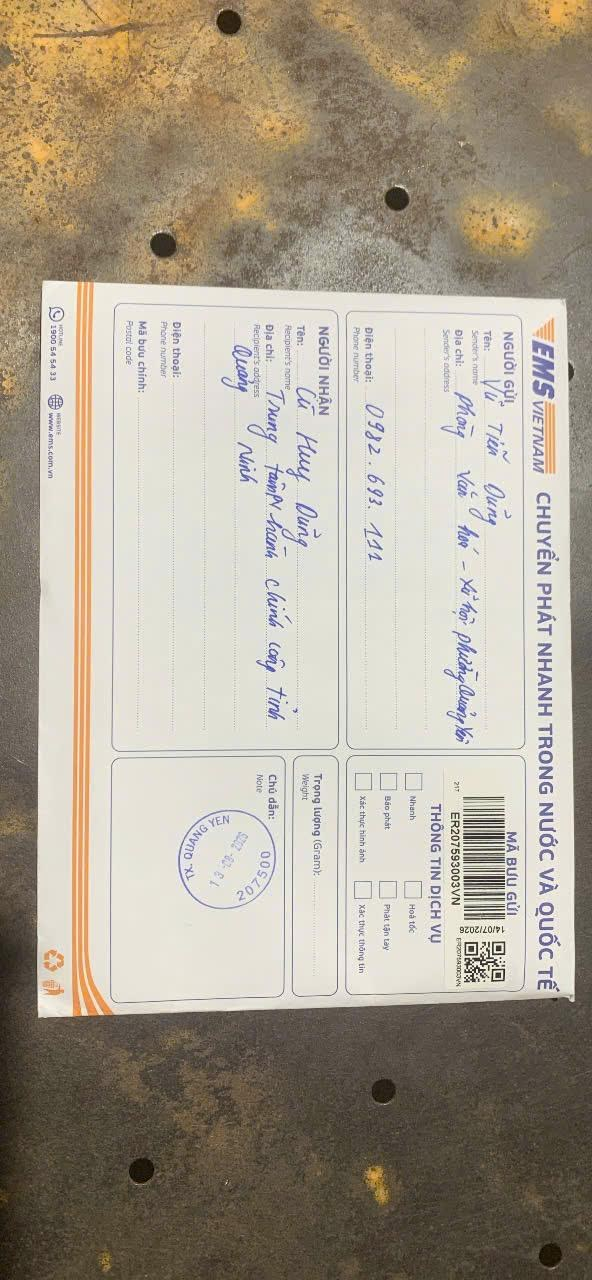
\includegraphics[height=6.2cm]{Images/fig3_1a.jpg}\hspace{0.6cm}
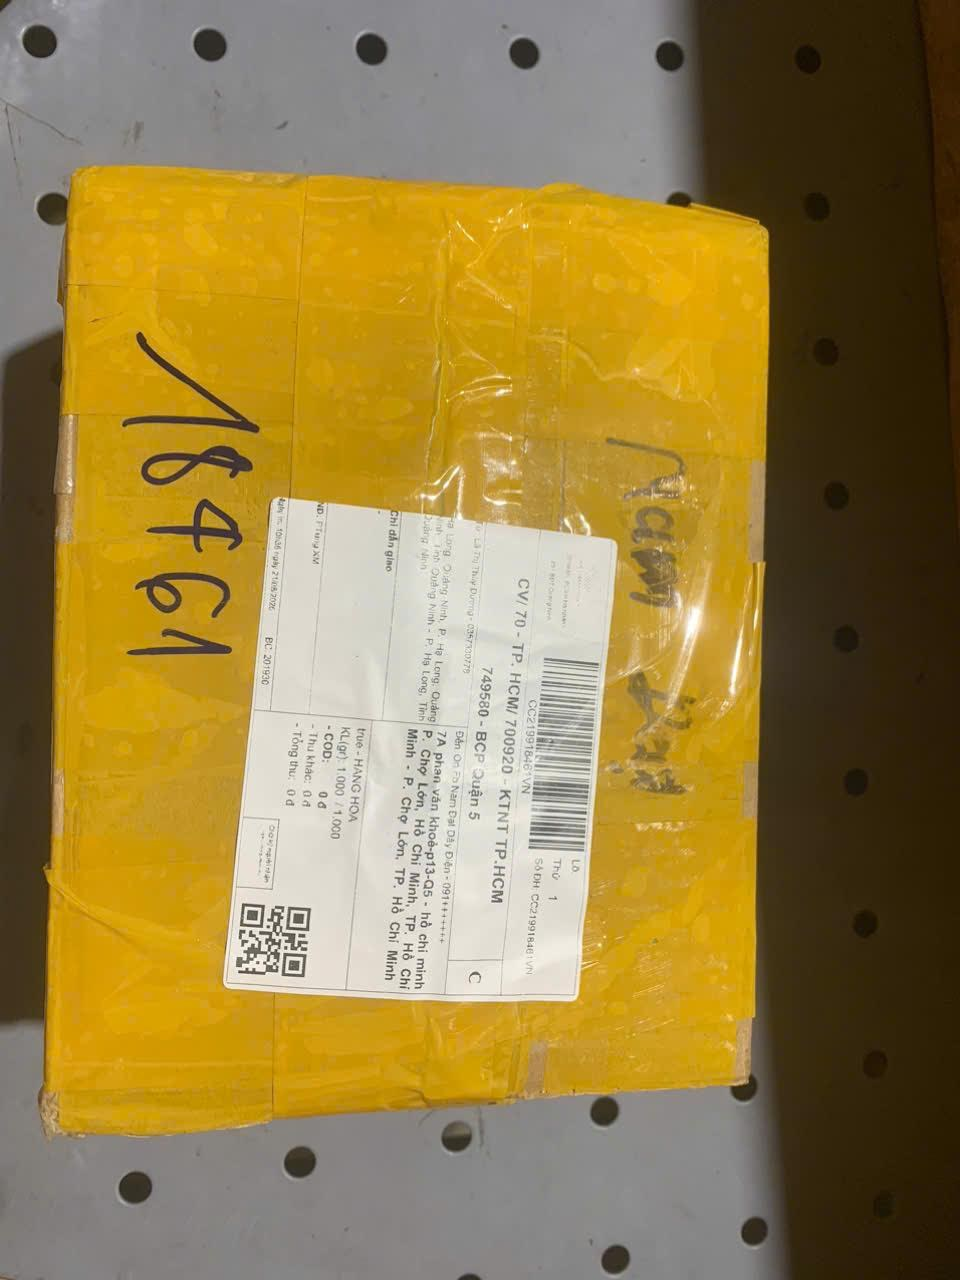
\includegraphics[height=6.2cm]{Images/fig3_1b.jpg}
\caption{Examples of annotated images in the Postal Item Dataset.}
\label{fig:postalitem}
\end{figure}

\begin{figure}[htbp]
\centering

\includegraphics[width=0.9\textwidth]{Images/fig3_2a.jpg}\\[0.4cm]

\includegraphics[width=0.9\textwidth]{Images/fig3_2b.png}
\caption[Examples of samples in Viet-Handwriting-OCR-v2]{Examples of samples in Viet-Handwriting-OCR-v2 \cite{viethandwriting}.}
\label{fig:viethandwriting}
\end{figure}

\begin{figure}[htbp]
\centering
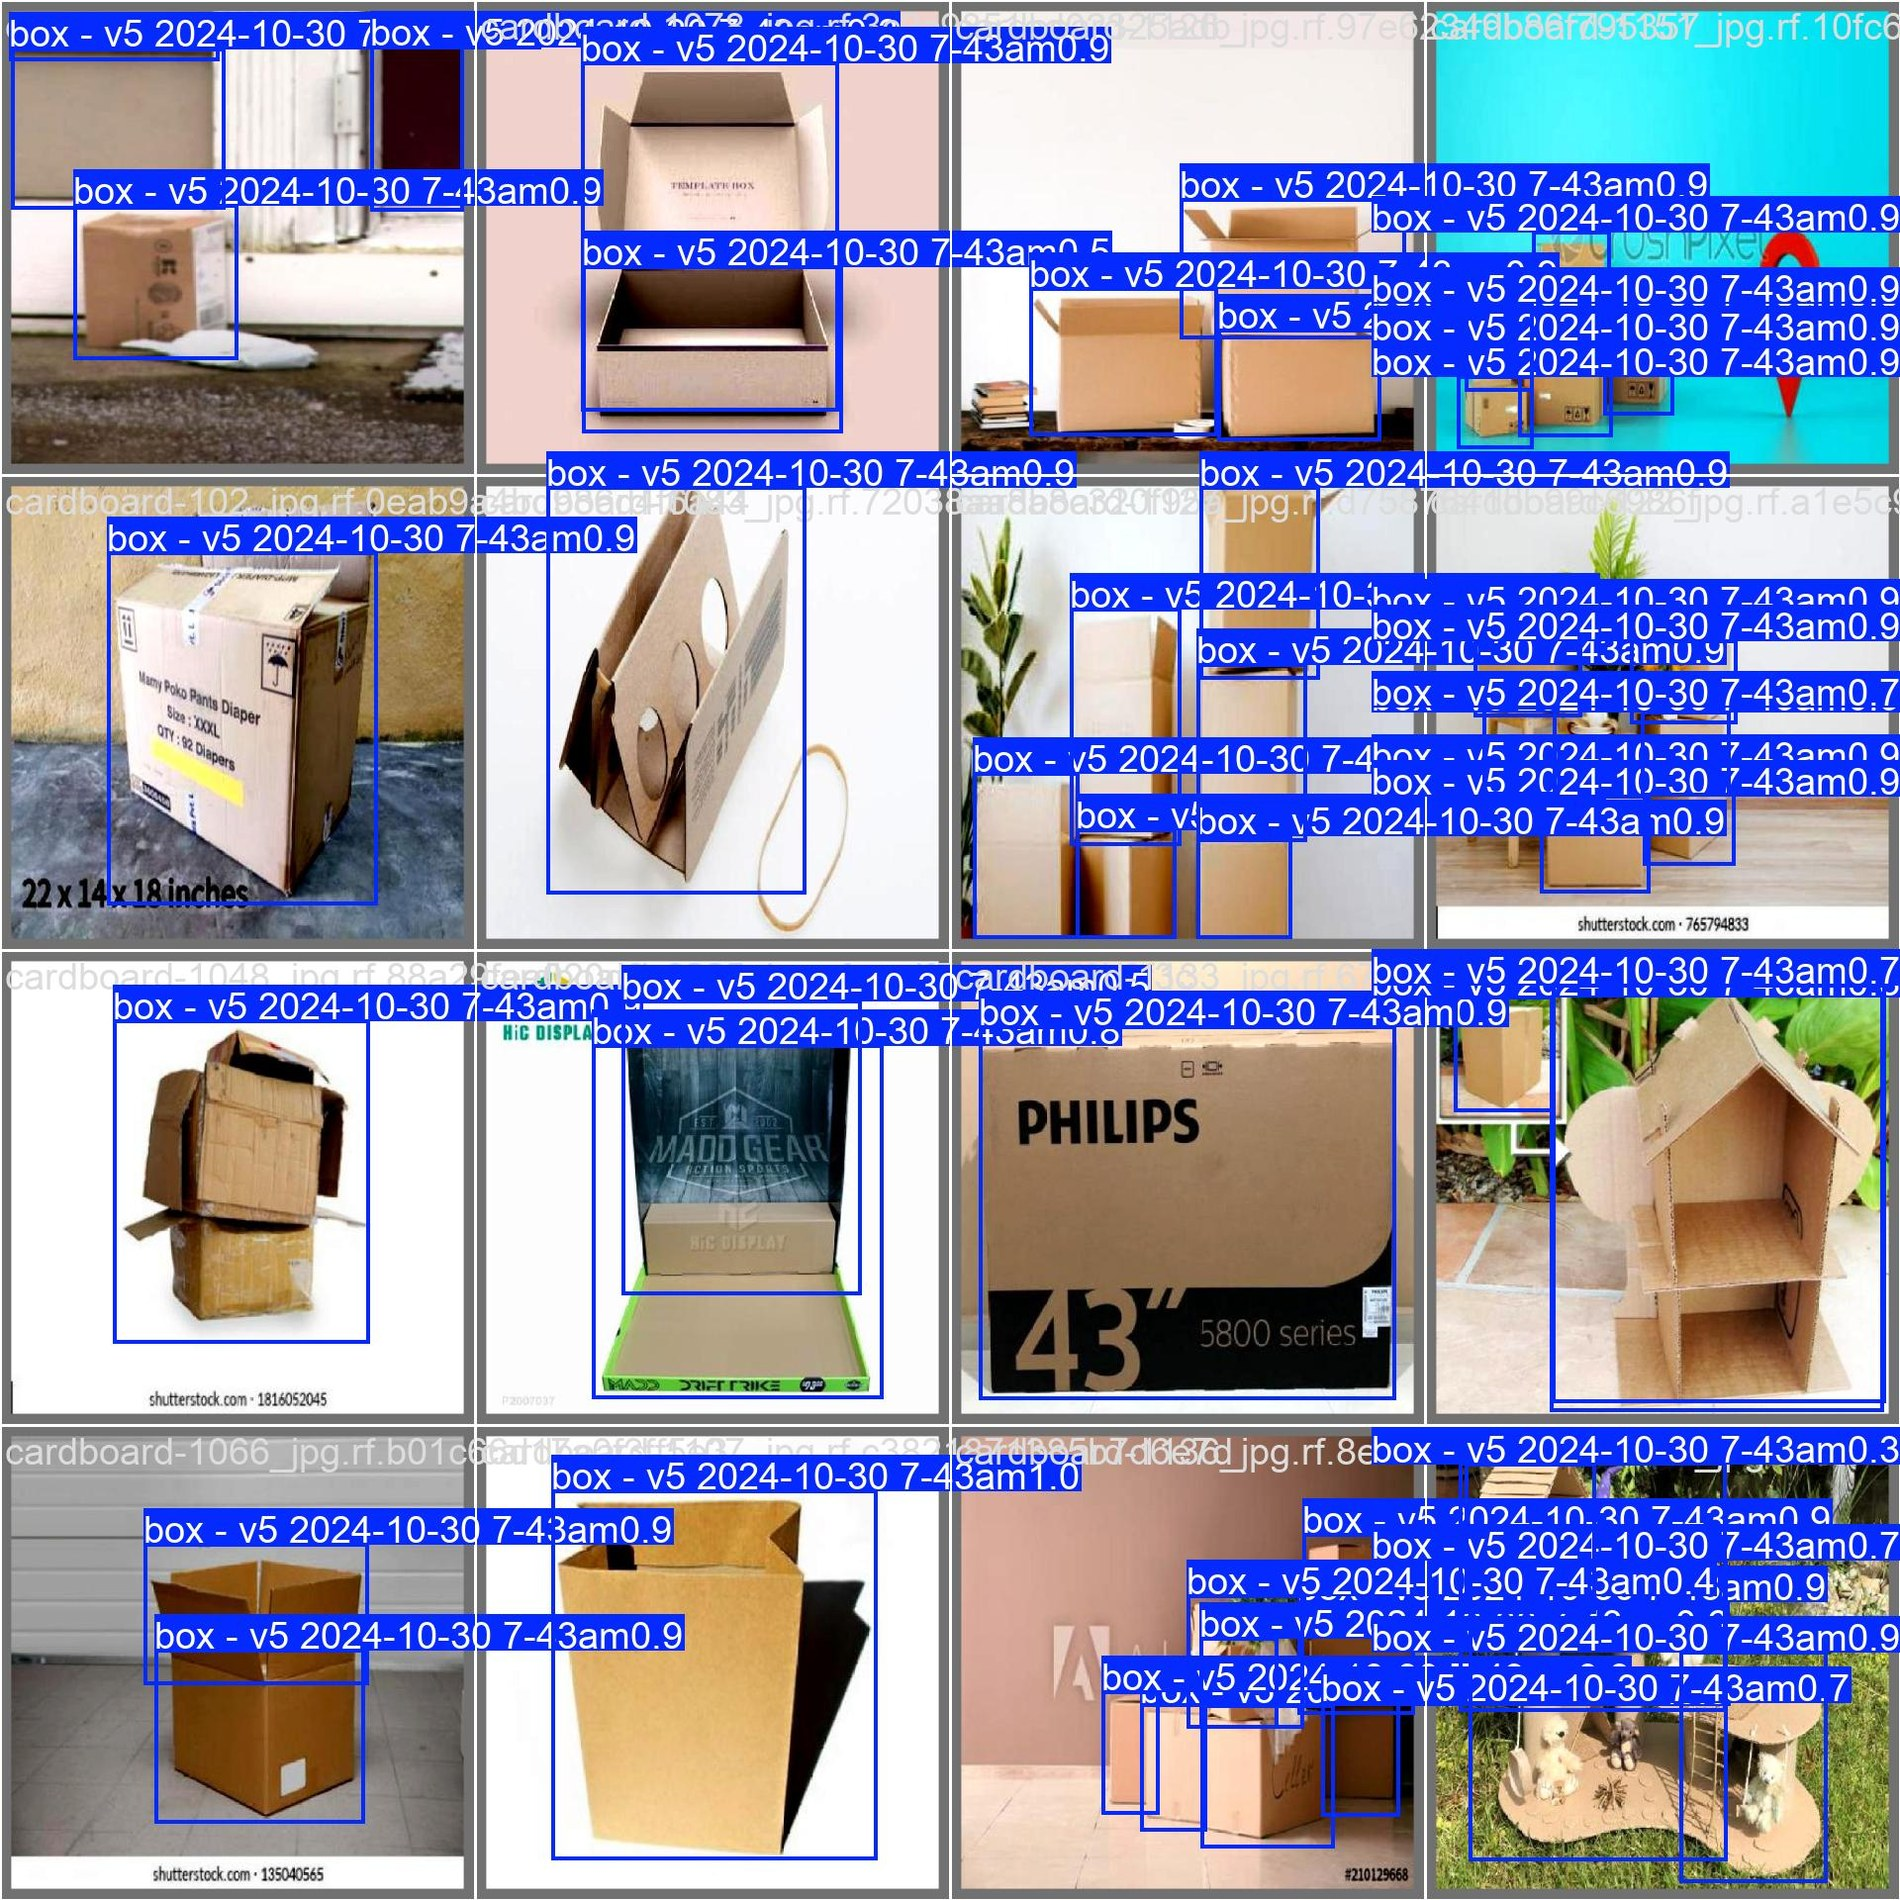
\includegraphics[width=0.72\textwidth]{Images/fig3_3.jpg}
\caption[Examples of annotated samples in the Cardboard Box Detection Dataset]{Examples of annotated samples in the Cardboard Box Detection Dataset \cite{cardboardbox2026}.}
\label{fig:cardboardbox}
\end{figure}

\begin{figure}[htbp]
\centering
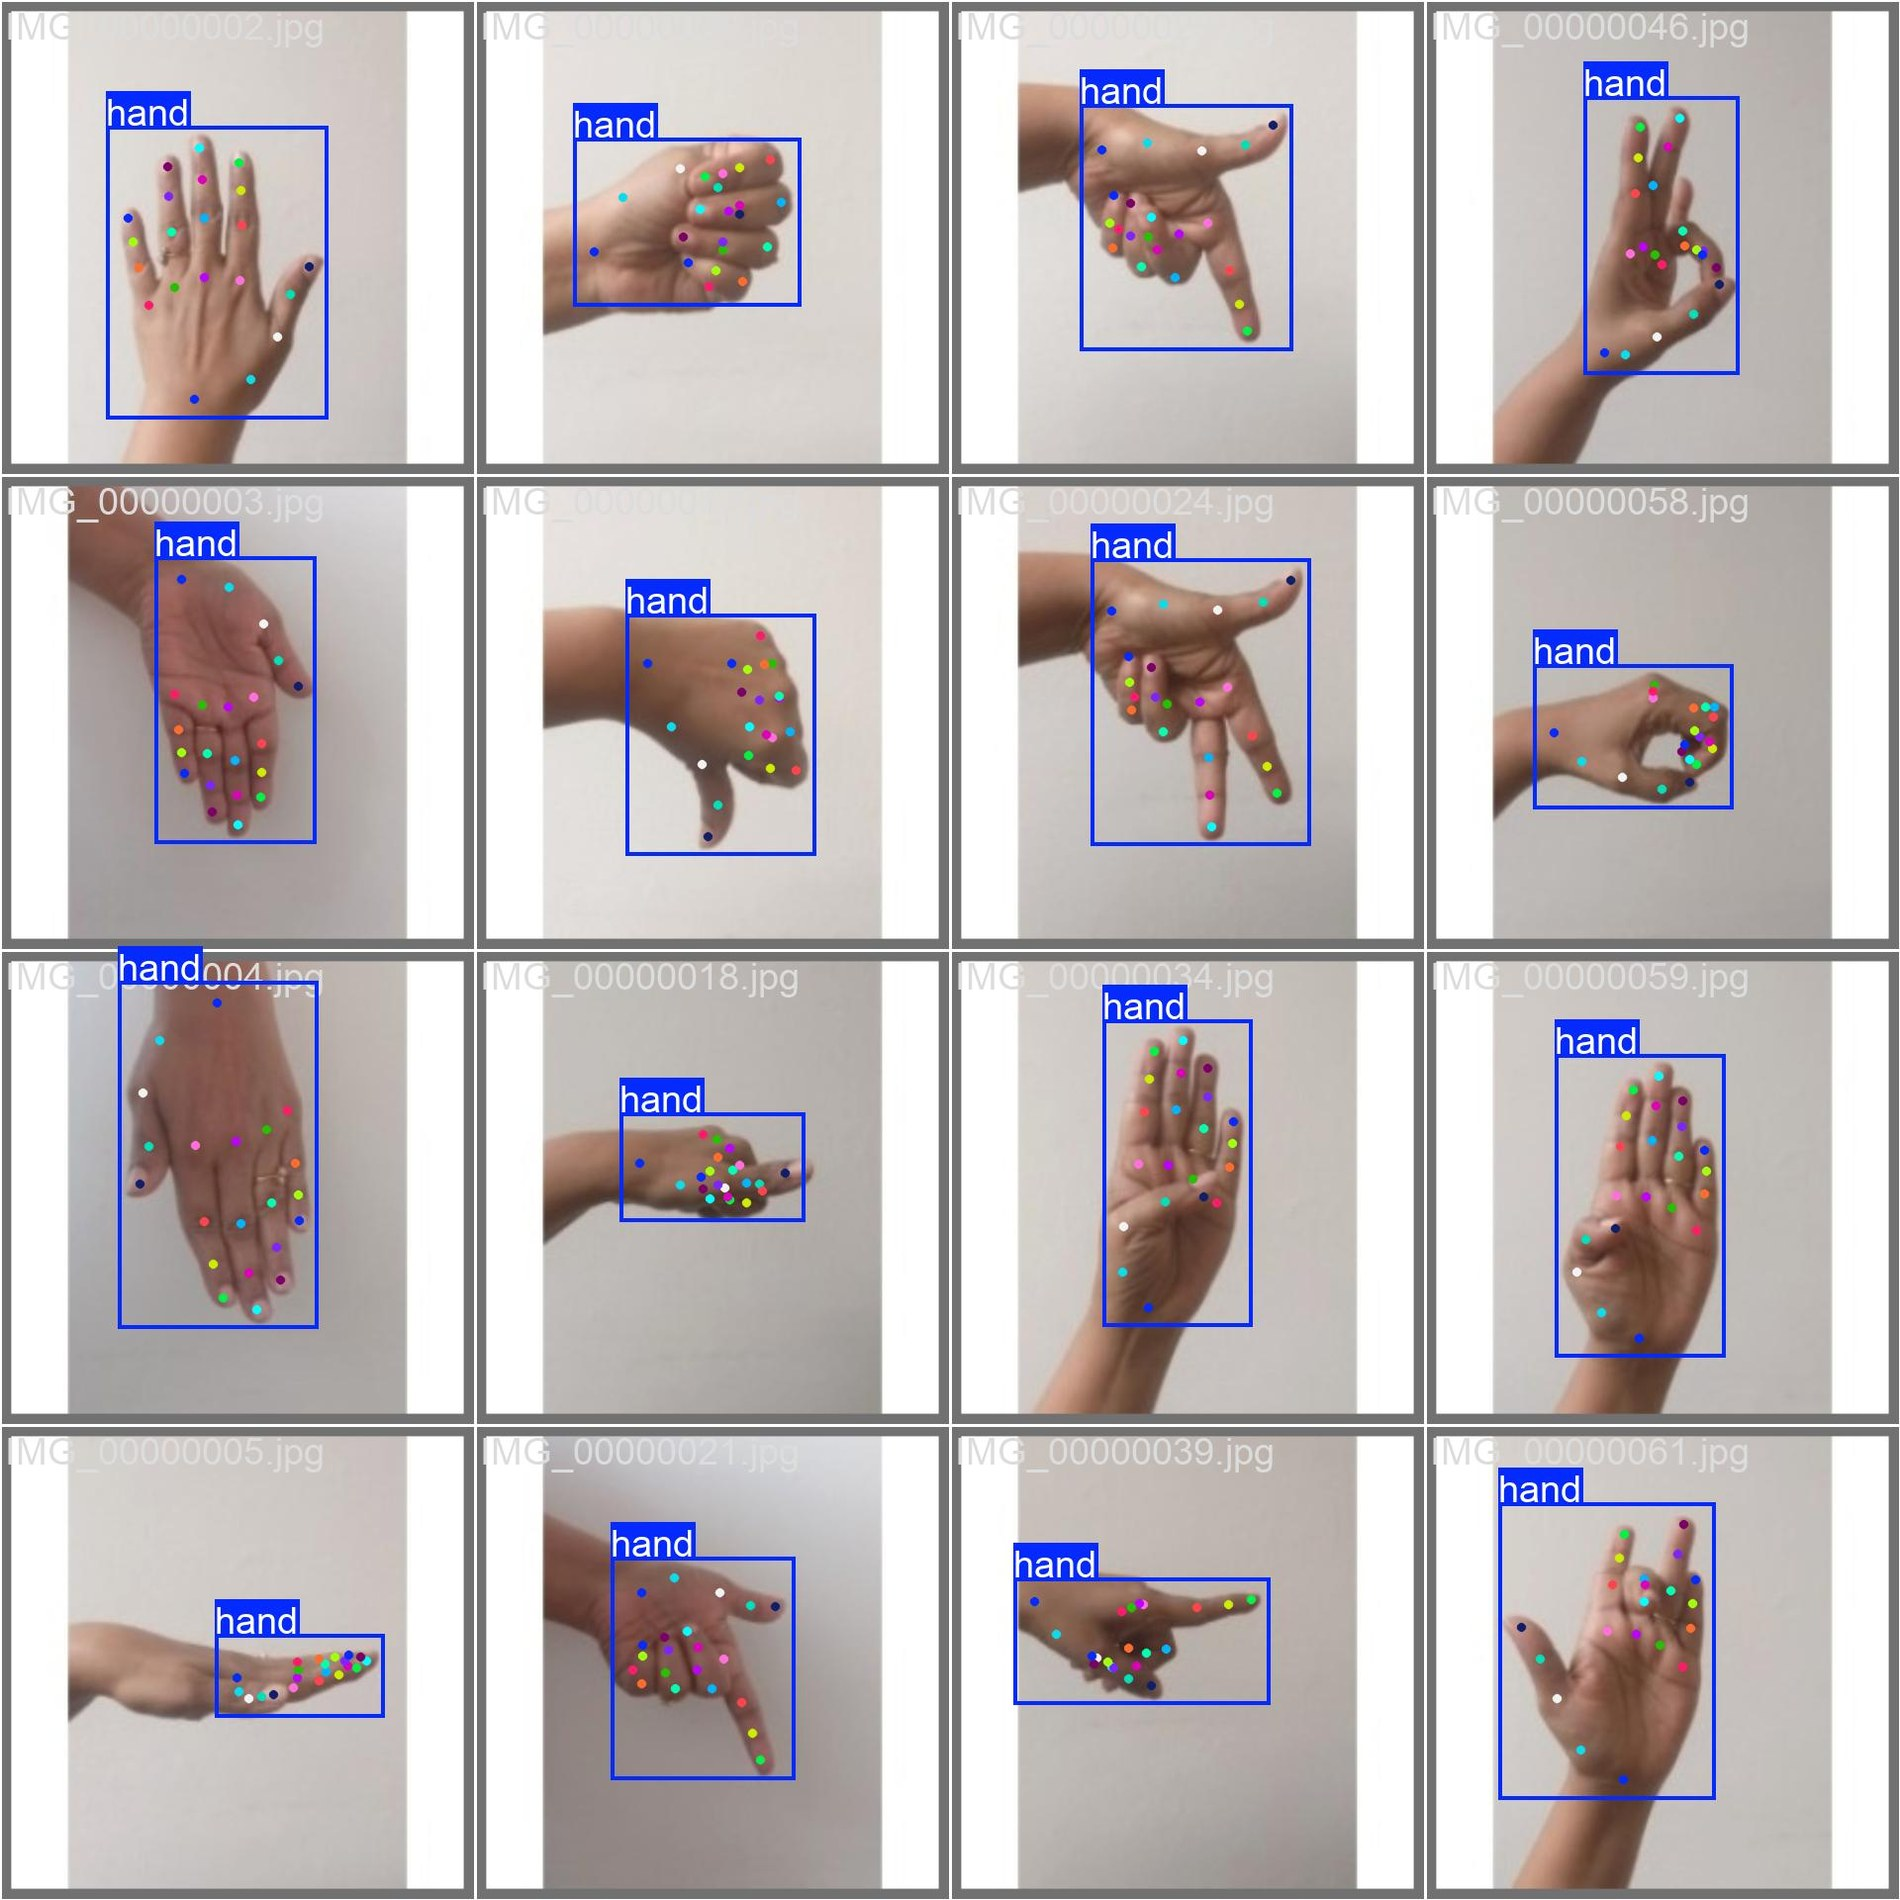
\includegraphics[width=0.72\textwidth]{Images/fig3_4.jpg}
\caption[Examples of annotated samples in the Hand Keypoints Dataset]{Examples of annotated samples in the Hand Keypoints Dataset \cite{ultralytics_hand}.}
\label{fig:handkeypoints}
\end{figure}

\section{Data Preprocessing and Cleaning}

Preprocessing was applied to the Postal Item Dataset only. The images in the training set were augmented to expand it from 351 to 1,050 images. The transformations include vertical flipping, rotation within $\pm 15^\circ$ and brightness adjustment within $\pm 15\%$. This process aims to increase the diversity of the training data. After augmentation, all images were resized to $640 \times 640$ pixels to provide a uniform input for the YOLO models.

For Box/Envelope Detection, the annotations were filtered to keep only the two classes \texttt{Label\_Box} and \texttt{Label\_Envelope}. For Information Region Detection, only images containing a \texttt{Label\_Box} were selected. The parcel region was cropped from the original image using the bounding box of the \texttt{Label\_Box} class, as illustrated in Figure~\ref{fig:cropinfo}. Cropping removes most of the background area and restricts the input data to the parcel surface.

\begin{figure}[htbp]
\centering
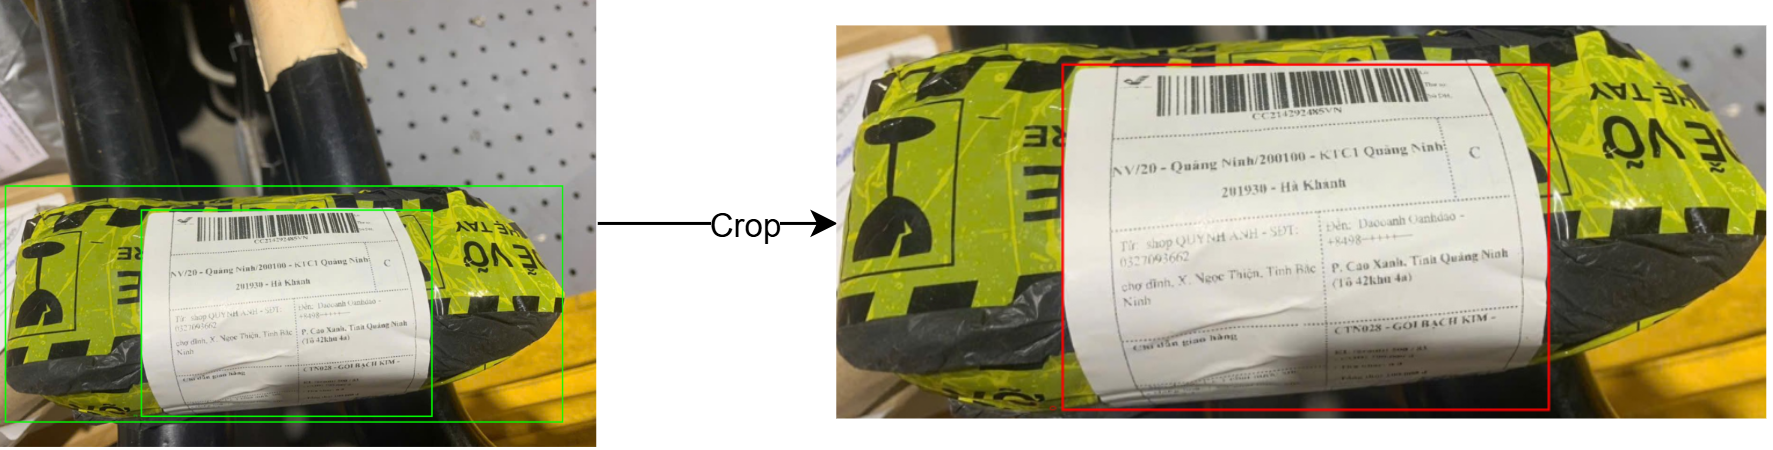
\includegraphics[width=\textwidth]{Images/fig3_5.png}
\caption{Illustration of the parcel region cropping process used to build the data for Information Region Detection.}
\label{fig:cropinfo}
\end{figure}

After the Label-Box region is cropped, the Label-info annotation in the original image can no longer be used directly, because the coordinate system of the image has changed. The bounding box coordinates of Label-info are therefore converted from the coordinate system of the original image to that of the cropped box image. From the bounding box $(x_c, y_c, W, H)$, the pixel coordinates are computed with Equation~\eqref{eq:pixelcoord}:

\begin{equation}
\label{eq:pixelcoord}
x = \left(x_c \pm \frac{W}{2}\right) W, \qquad
y = \left(y_c \pm \frac{H}{2}\right) H
\end{equation}

where $x_c$ and $y_c$ are the centre coordinates and $W$ and $H$ are the width and height of the image. From these, the edge coordinates of Label-info $[x_1{:}x_2,\, y_1{:}y_2]$ and of Label-box $[b_{x1}{:}b_{x2},\, b_{y1}{:}b_{y2}]$ are derived. After the box is cropped, the info coordinates are shifted into the new coordinate system with Equation~\eqref{eq:coordshift}:

\begin{equation}
\label{eq:coordshift}
x' = x - b_x, \qquad y' = y - b_y
\end{equation}

Once the four edge coordinates of the new Label-info are obtained, they are normalized back into YOLO format, and the class identifier is changed from 2, denoting \texttt{Label\_info}, to 0.

The remaining three datasets are fed into the models without any additional preprocessing beyond the default procedures of their sources.

\section{Summary of Data Processing}

The four datasets cover the main tasks of the system: distinguishing parcels from envelopes, detecting the information region, recognizing handwriting, detecting parcels and identifying hand regions. Preprocessing was limited to augmentation, resizing, annotation filtering, cropping and coordinate conversion on the self-collected Postal Item Dataset; the three public datasets were used as provided. The splits applied to each model are reported in Section~\ref{sec:training} together with the training configuration.

The Postal Item Dataset allows the models to learn the basic features needed to distinguish envelopes, parcels and information regions. However, the number of images is still limited. Cases such as deformed parcels or parcels with elongated shapes do not appear often enough, and the envelope images were mostly captured in the same environment and in a flat position, which reduces the diversity of the data.

Viet-Handwriting-OCR-v2 contains a relatively large number of samples and is suitable for fine-tuning the TrOCR model. However, the data was not built specifically for postal shipping forms, and the team did not apply augmentation to simulate real photographs. The model may therefore struggle with slanted handwriting, smudged ink or low-quality images.

Overall, the datasets provide a basis for training and evaluating each component of the system. Nevertheless, the quantity and diversity of real data from the post office still need to be expanded in order to cover deployment conditions more thoroughly.

\chapter{Methodology}
\label{chap:methodology}

This chapter describes the proposed system. It begins with the workflow of the current manual process and the automated workflow that replaces part of it, then presents the architecture of the three functional groups, the algorithm of each module, the training configuration and the implementation details.

The system comprises six main functions:

\begin{itemize}
    \item \textbf{Box/Envelope Detection:} determines whether the postal item is a parcel or an envelope.
    \item \textbf{Information Region Detection:} locates the region containing information on the parcel surface.
    \item \textbf{Handwriting Recognition:} detects text regions, recognizes the handwriting and converts the output into structured data.
    \item \textbf{Dimension Measurement Using Computer Vision:} measures parcel dimensions with two webcams, YOLO and image processing.
    \item \textbf{Dimension Measurement Using Ultrasonic Sensors:} measures dimensions with three ultrasonic sensors and an ESP32.
    \item \textbf{Shipping Fee Calculation:} normalizes province and city names, determines the route, computes the chargeable weight and calculates the shipping fee.
\end{itemize}

\section{Business Process Analysis}
\label{sec:bpa}

The current manual workflow at the acceptance counter is illustrated in Figure~\ref{fig:currentprocess}: read the information, enter the data, weigh the item, read the weight, enter the weight, measure the dimensions, enter the dimensions, determine the chargeable weight, select the service, calculate the fee, check and confirm.

\begin{figure}[htbp]
\centering
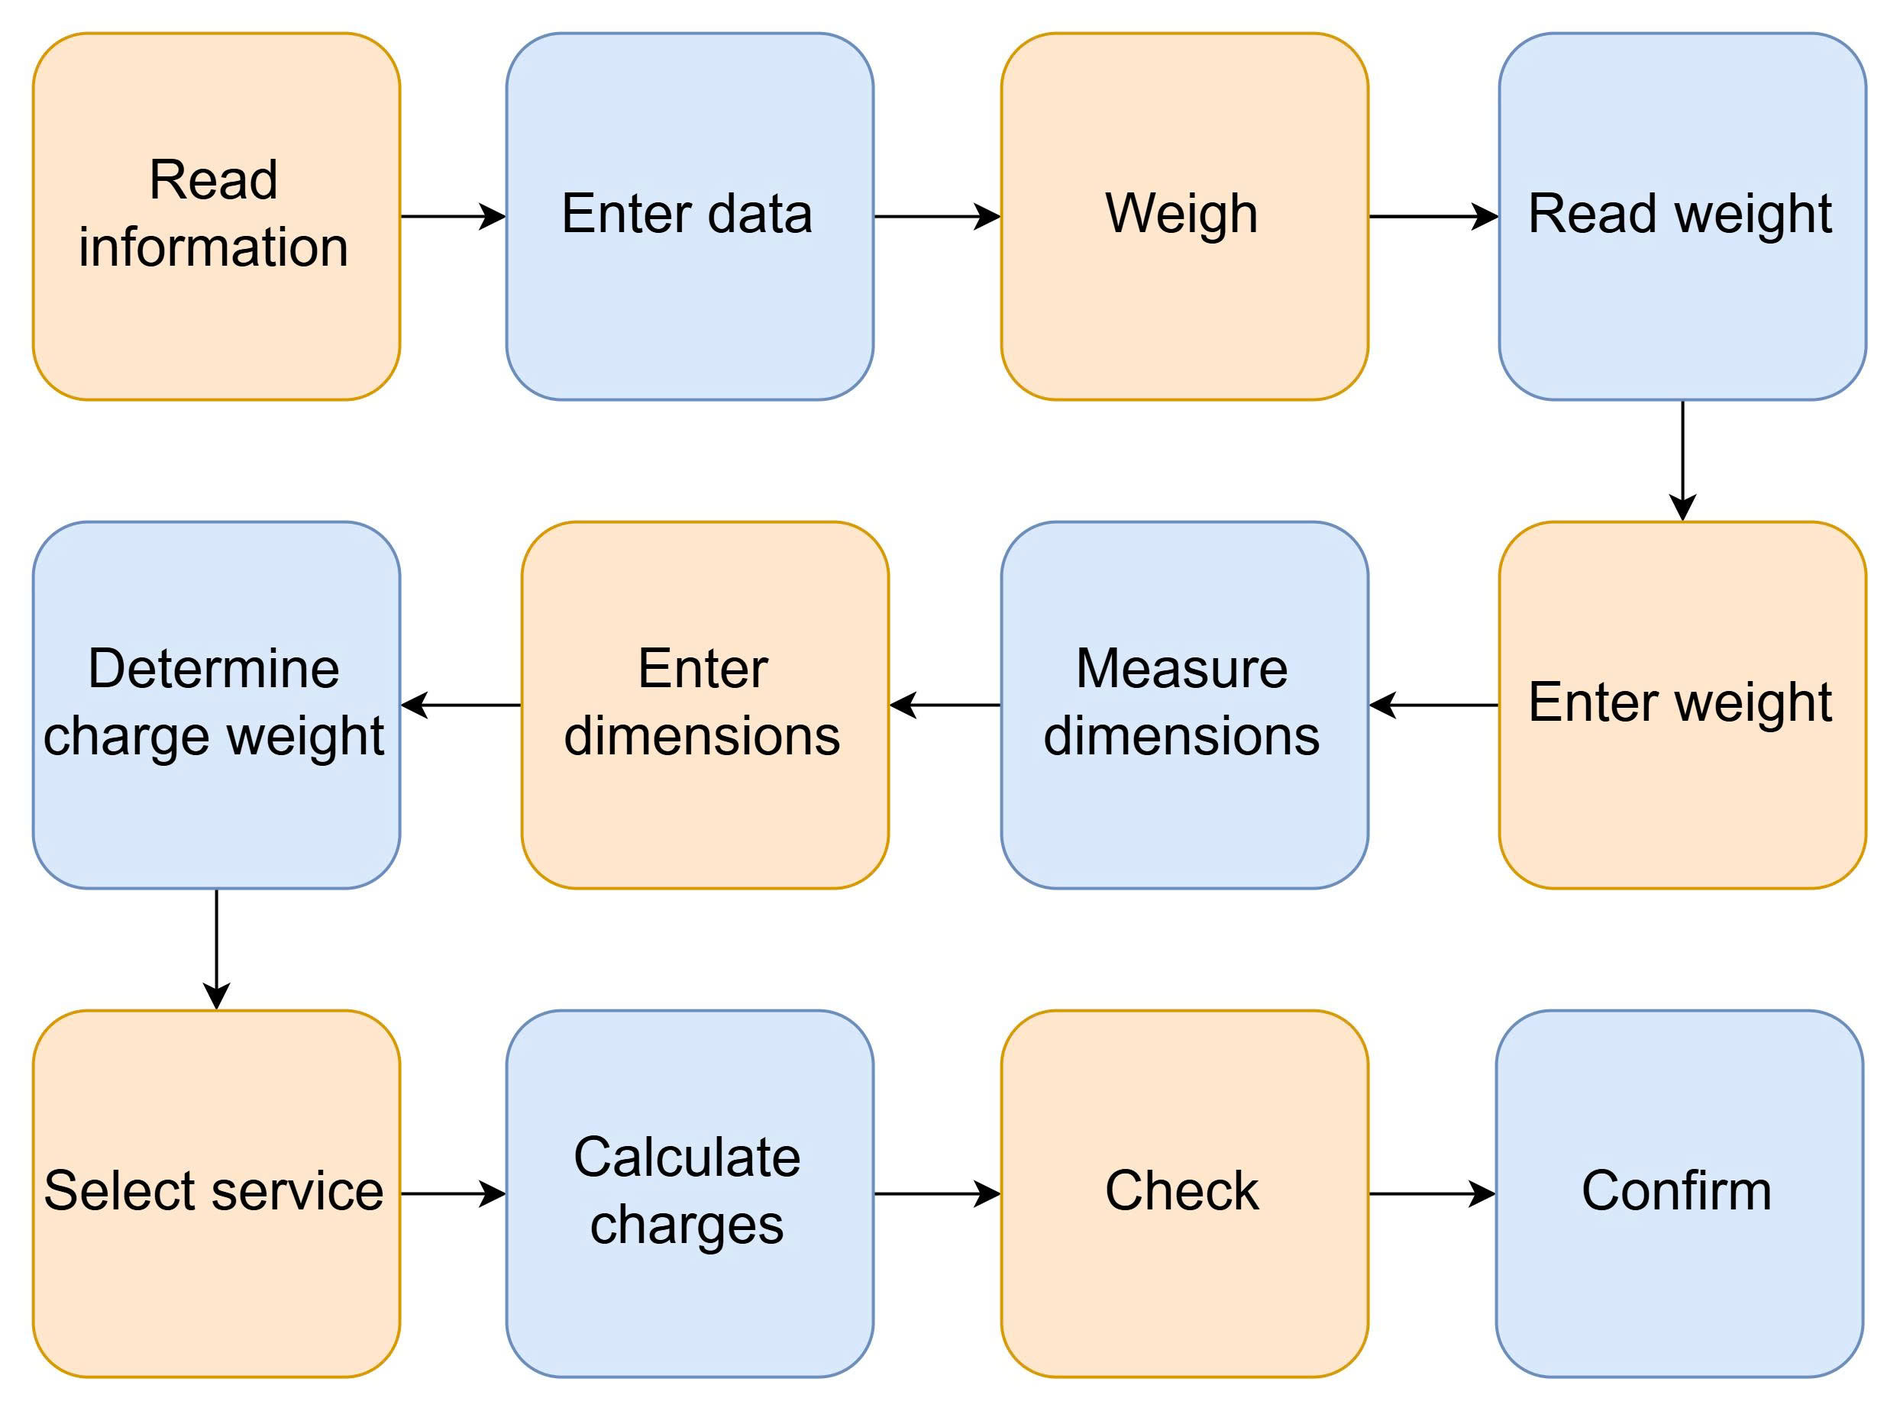
\includegraphics[width=0.92\textwidth]{Images/fig4_1.png}
\caption{Current postal item handling process at the acceptance counter.}
\label{fig:currentprocess}
\end{figure}

In practice, completing a typical postal transaction currently takes about 6--8 minutes per item. Within that time the clerk must carry out many consecutive steps: receiving the request; reading or asking for sender and receiver information; entering names, phone numbers and addresses; checking the contents; weighing the item; measuring dimensions where required; entering the parameters into the software; determining the chargeable weight; selecting the service; determining the base fee, surcharges and value-added services; re-checking the information; printing the label or shipping form; collecting payment and completing the transaction. This description is based on the team's own observation of the acceptance counter.

The proposed system automates three groups of these steps. Reading information and entering data are replaced by automatic extraction of the information on the postal item using a handwriting OCR model. Measuring and entering dimensions are replaced by automatic parcel dimension measurement using USB webcams or ultrasonic sensors. Determining the chargeable weight, selecting the service and calculating the fee are replaced by automatic computation of the volumetric weight, service type determination and fee calculation.

\section{Overall Workflow}

Figure~\ref{fig:workflow} presents the processing flow of the proposed system, from receiving the input image to saving the result in the database.

\begin{figure}[htbp]
\centering
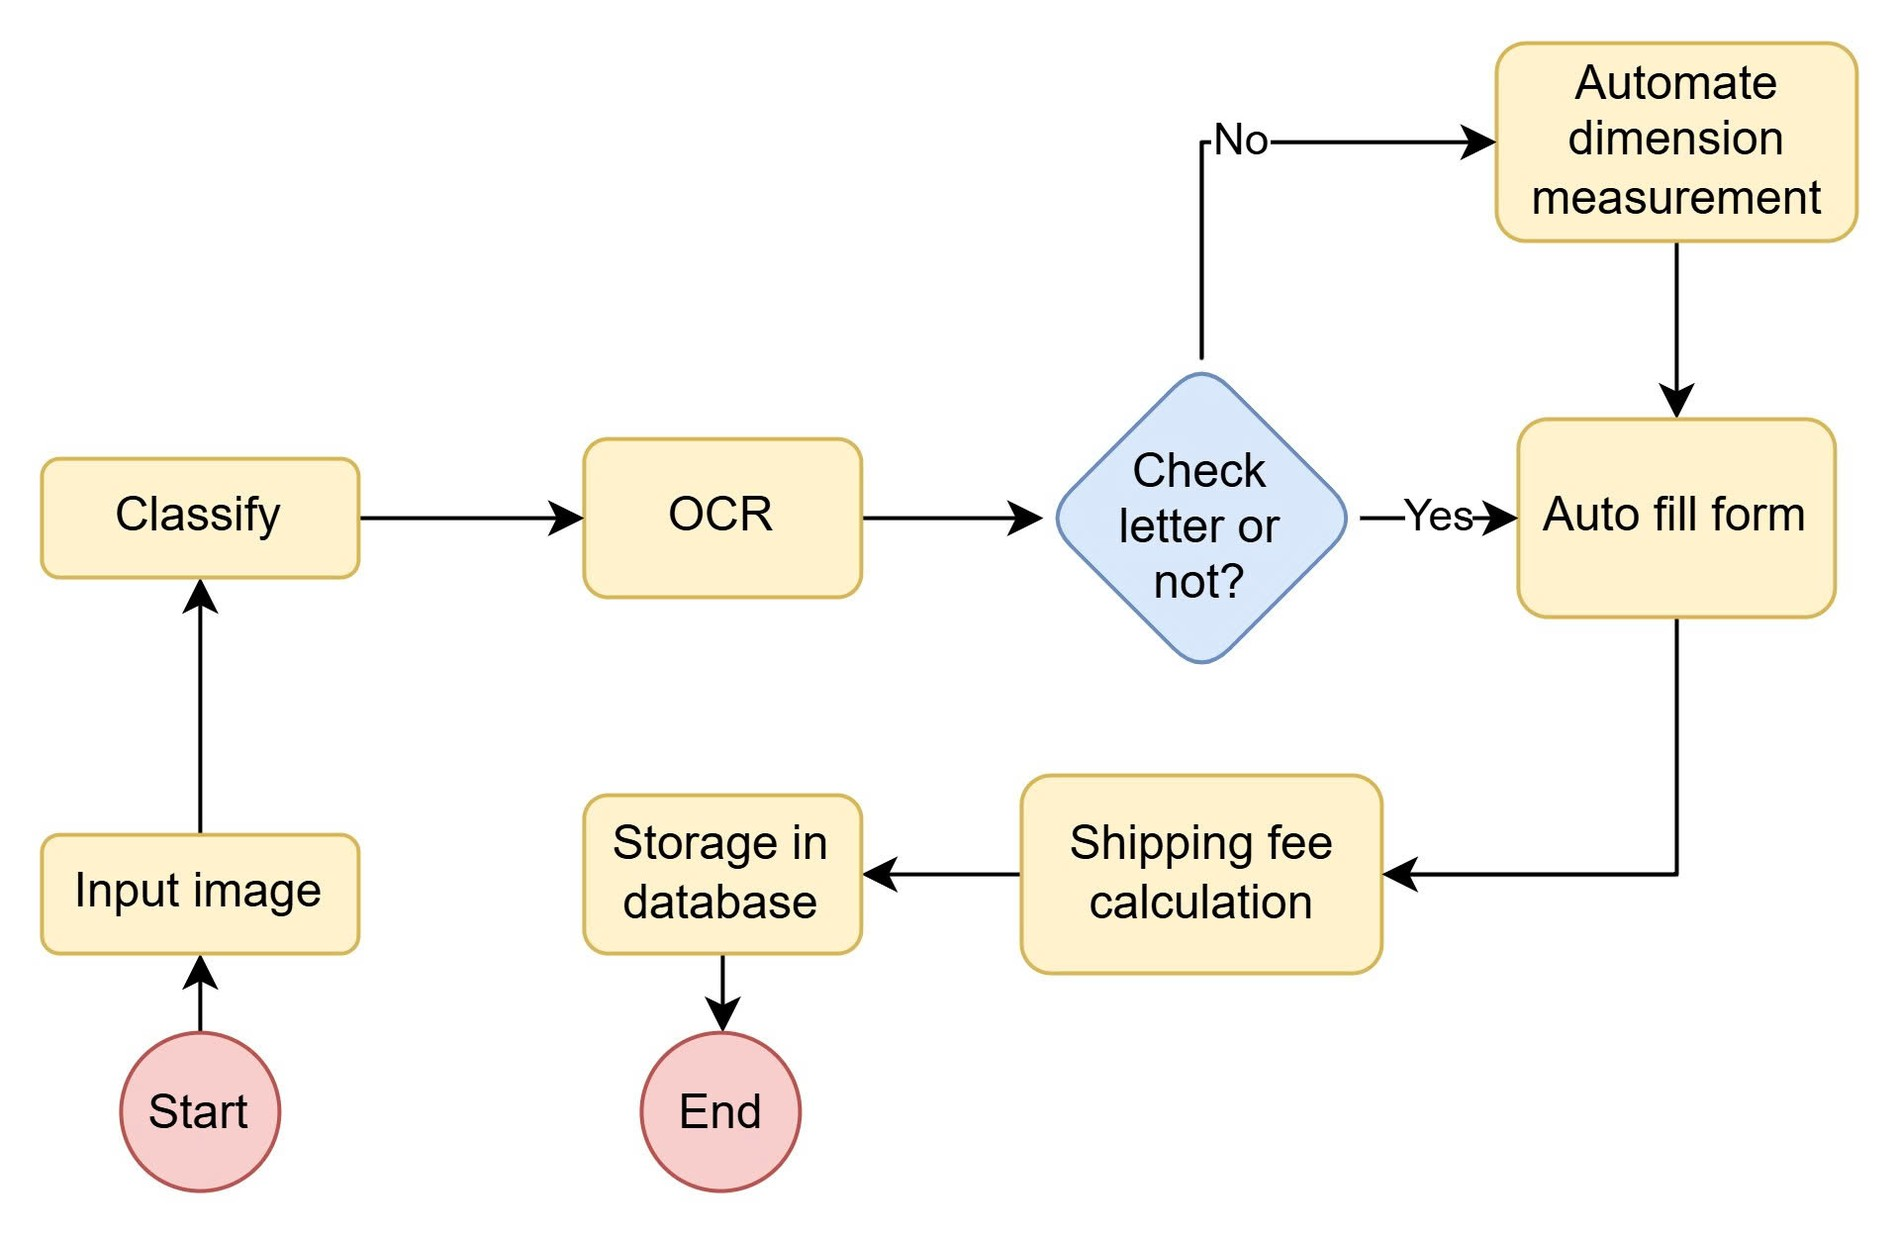
\includegraphics[width=\textwidth]{Images/fig4_2.jpg}
\caption{Overall processing workflow of the proposed system.}
\label{fig:workflow}
\end{figure}

First, the system receives the postal item image and uses the Box/Envelope Detection module to determine whether the input is a parcel or an envelope. The image is then passed through the OCR pipeline to detect and recognize the handwritten information. Both item types use the same OCR pipeline, but the way the input region is prepared differs. For envelopes, the envelope region is cropped and passed directly to the text region detection step. For parcels, the system additionally uses Information Region Detection to locate and crop the information label region before recognizing the handwriting.

The classification result is retained in order to determine the subsequent processing path. If the item is an envelope, the system skips the dimension measurement step and passes the OCR result to the form. If the item is a parcel, the system additionally performs dimension measurement using webcams or ultrasonic sensors before filling in the form.

Once the form has been filled in, the clerk enters the actual weight and selects the service. The system uses the province information, the weight and the dimensions to calculate the shipping fee. Finally, the transaction information and the fee calculation result are saved to the database.

\section{System Architecture}

Based on the workflow presented above, the system components are organized into three functional groups: postal information extraction and recognition, webcam-based dimension measurement, and ultrasonic-sensor-based dimension measurement. This section presents the structure and the connections between the components of each group; their processing procedures are presented in Section~\ref{sec:algorithm_description}.

\subsection{Postal Information Extraction and Recognition}

Figure~\ref{fig:infoarch} presents the combination of the three functions Box/Envelope Detection, Information Region Detection and Handwriting Recognition.

\begin{figure}[htbp]
\centering
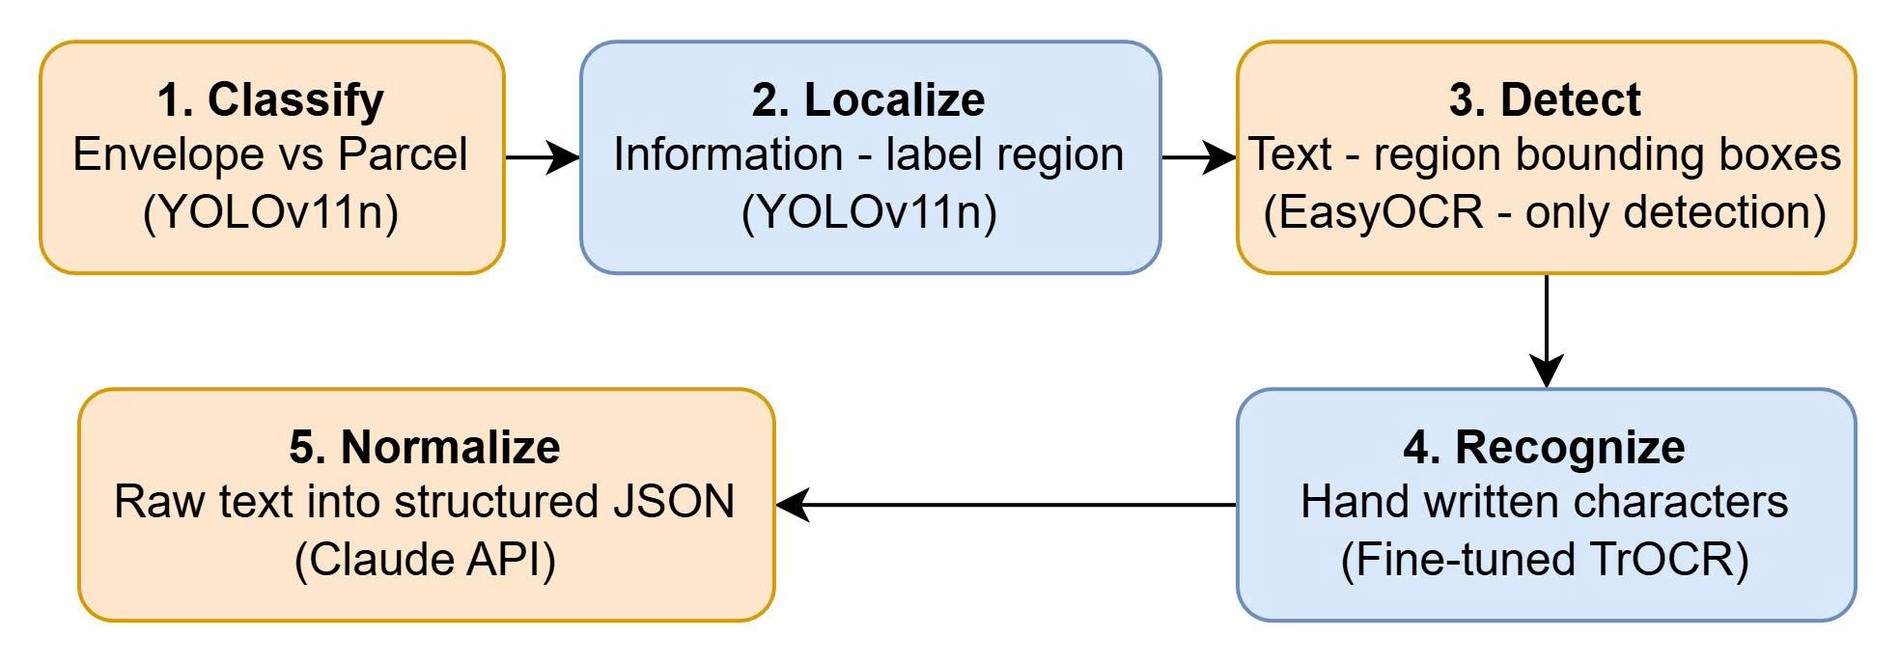
\includegraphics[width=\textwidth]{Images/fig4_3.jpg}
\caption{Architecture of the postal information extraction and recognition module.}
\label{fig:infoarch}
\end{figure}

First, YOLO11n determines whether the item is a parcel or an envelope. This result decides how the image region to be processed is identified. For parcels, a second YOLO11n model locates the information label region on the parcel surface; for envelopes, the envelope image region is used directly. Once the information region has been identified, EasyOCR detects the regions containing text and returns their bounding boxes. Each text region is then passed to the fine-tuned TrOCR model to recognize the handwritten content. Finally, the recognized text is reordered and converted into structured JSON data through the Claude API.

\subsection{Webcam-Based Dimension Measurement}

The architecture of the webcam-based measurement system is shown in Figure~\ref{fig:webcamarch}. It consists of four main components.

\begin{figure}[htbp]
\centering
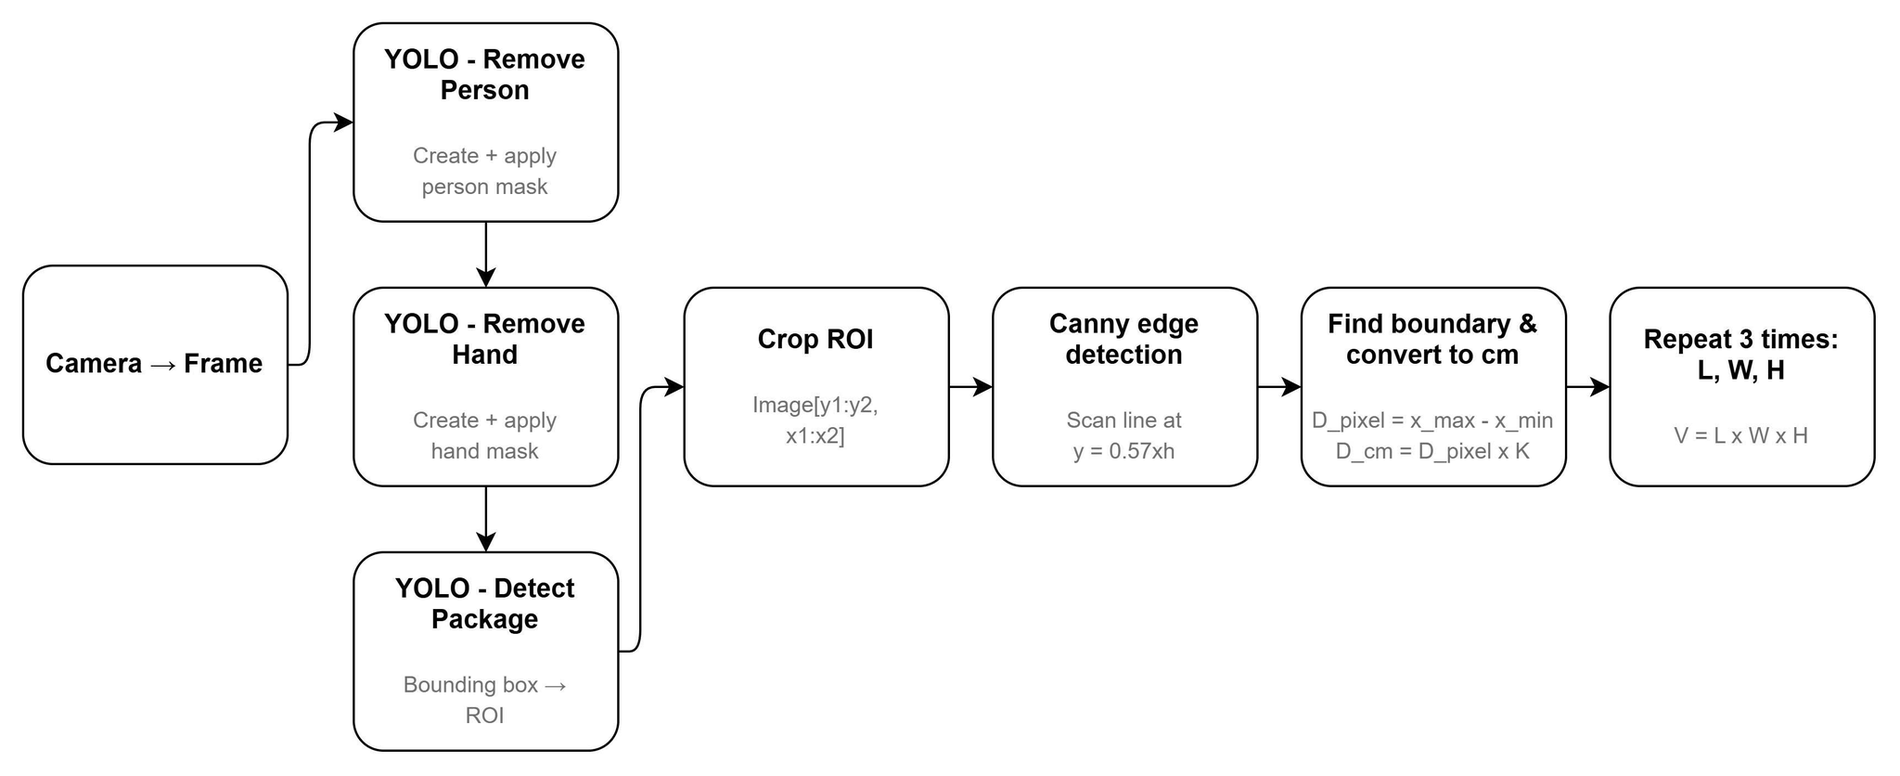
\includegraphics[width=\textwidth]{Images/fig4_4.png}
\caption{Architecture of the two-webcam dimension measurement system.}
\label{fig:webcamarch}
\end{figure}

\begin{itemize}
    \item \textbf{YOLO26n Person Detection:} detects human body regions that may appear in the image.
    \item \textbf{YOLO Hand Keypoints:} detects hands and their keypoints in order to identify the regions to be removed.
    \item \textbf{YOLO Package Detection:} determines the bounding box of the parcel and creates the region of interest.
    \item \textbf{Dimension Measurement:} detects edges within the region of interest, determines the dimensions in pixels and converts them into centimetres.
\end{itemize}

The person and hand regions are masked before parcel boundary detection. This step limits cases in which the body or hand is mistaken for part of the parcel boundary. The bounding box returned by YOLO Package Detection is used to crop the region of interest, after which Canny edge detection identifies the edges used for measurement \cite{canny1986}.

\subsection{Ultrasonic-Sensor-Based Dimension Measurement}

The architecture of the ultrasonic measurement system is shown in Figure~\ref{fig:ultrasonicarch}. It consists of three main blocks.

\begin{figure}[htbp]
\centering
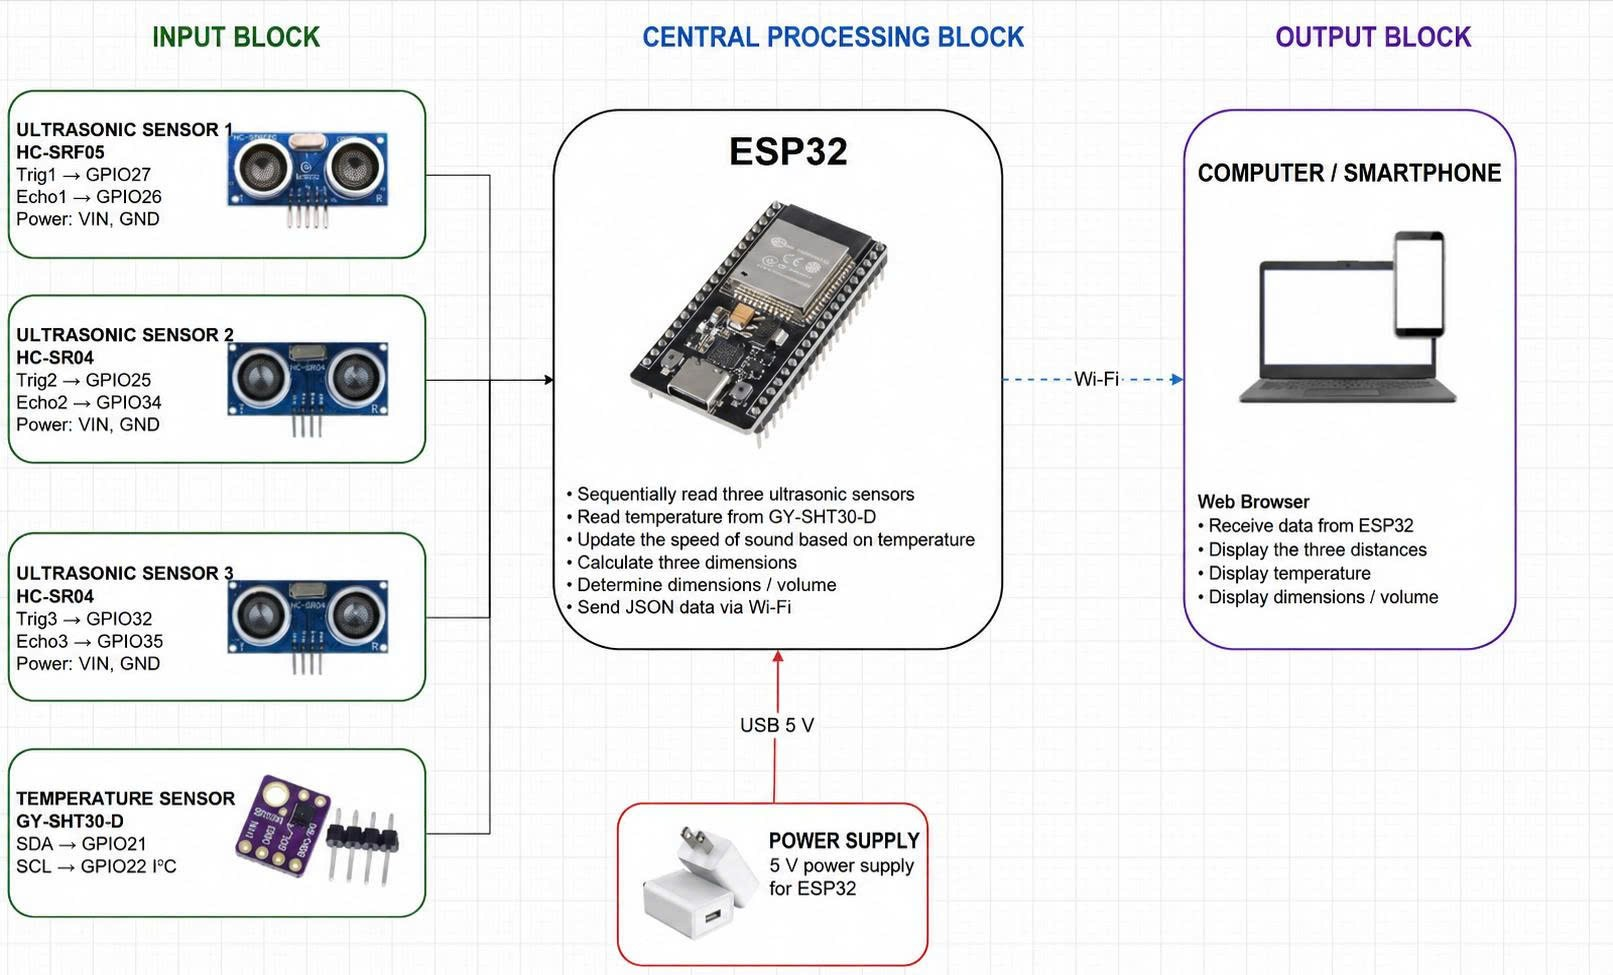
\includegraphics[width=\textwidth]{Images/fig4_5.jpg}
\caption{Architecture of the ultrasonic-sensor dimension measurement system.}
\label{fig:ultrasonicarch}
\end{figure}

The input block contains three ultrasonic sensors for distance measurement and an \mbox{SHT30-D} sensor for ambient temperature measurement. The sensor data is transmitted to the ESP32 in the central processing block. The ESP32 reads the three ultrasonic sensors in turn, updates the speed of sound according to the temperature, determines the three distances and computes the length, width, height and volume of the parcel. The result is packaged as JSON and sent over Wi-Fi. The output block is a browser on a computer or phone; the interface receives the data from the ESP32 and displays the temperature, the three distances, and the dimensions and volume of the parcel.

\section{Algorithm Description}
\label{sec:algorithm_description}

\subsection{Box/Envelope Detection}

The study uses YOLO11n to detect and distinguish parcels from envelopes. Rather than training from scratch, the model is initialized from the pretrained weights \texttt{yolo11n.pt} and then fine-tuned on the Postal Item Dataset. The model uses two classes, \texttt{Label\_Box} and \texttt{Label\_Envelope}; the \texttt{Label\_info} class is not used when training this model because it is not needed for distinguishing the two item types.

\begin{figure}[htbp]
\centering
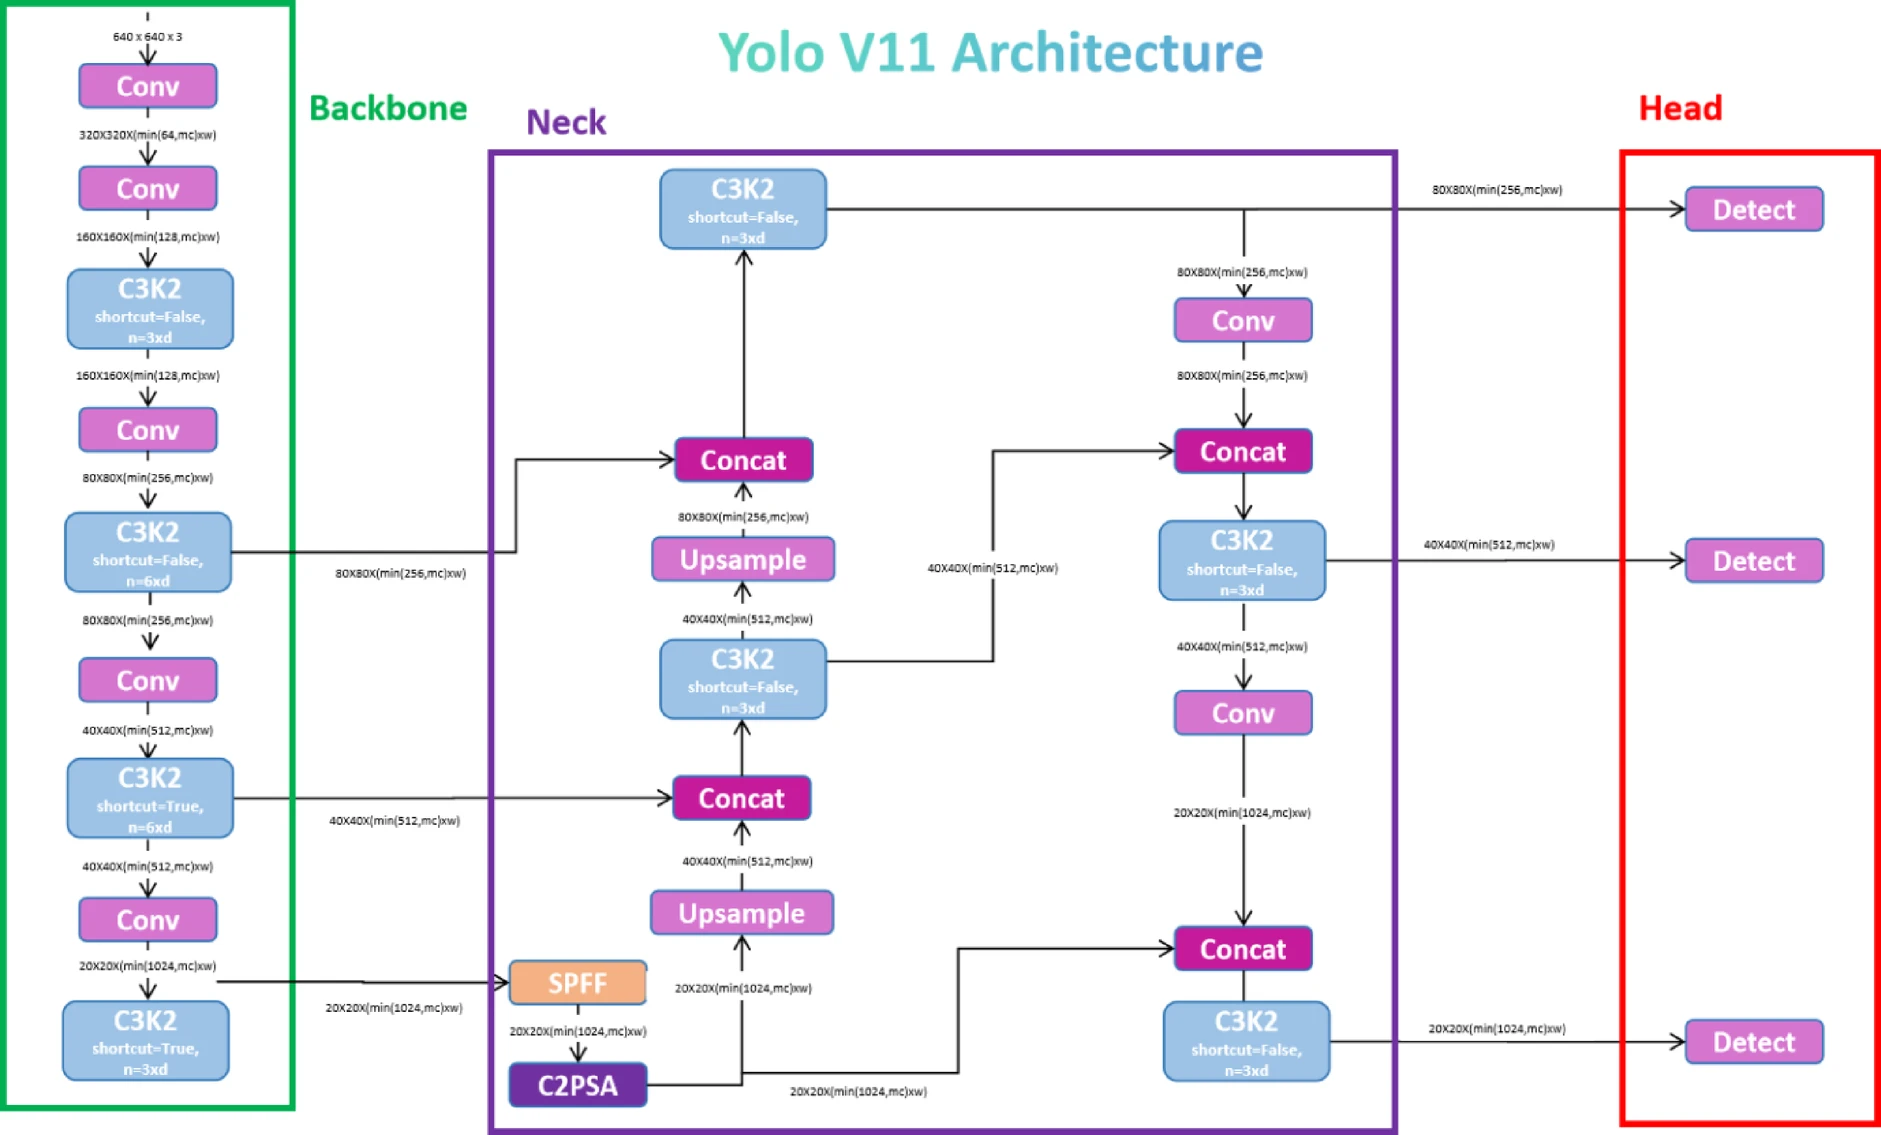
\includegraphics[width=\textwidth]{Images/fig4_6.png}
\caption{General architecture of YOLO11n.}
\label{fig:yolo11n}
\end{figure}

As shown in Figure~\ref{fig:yolo11n}, YOLO11n is a single-stage object detection model whose operation consists of three main steps: feature extraction, object prediction and result post-processing. At a high level, the architecture has three components \cite{ultralytics_yolo11}:

\begin{itemize}
    \item \textbf{Backbone:} extracts features from the input image. The early layers learn basic features such as edges, shapes and textures, while the deeper layers produce features with a higher semantic level.
    \item \textbf{Neck:} combines the extracted features across multiple levels and scales.
    \item \textbf{Detection head:} uses the combined features to predict bounding boxes, class labels and confidence scores.
\end{itemize}

The model output consists of a bounding box giving the position and size of the object, a class indicating whether the object is a \texttt{Label\_Box} or a \texttt{Label\_Envelope}, and a confidence score. The overlap between the predicted bounding box and the ground-truth bounding box is measured by the intersection over union, defined in Equation~\eqref{eq:iou}:

\begin{equation}
\label{eq:iou}
\mathrm{IoU} = \frac{\mathrm{Area}\left(B_{\mathrm{pred}} \cap B_{\mathrm{gt}}\right)}{\mathrm{Area}\left(B_{\mathrm{pred}} \cup B_{\mathrm{gt}}\right)}
\end{equation}

where $B_{\mathrm{pred}}$ is the bounding box predicted by the model and $B_{\mathrm{gt}}$ is the annotated ground-truth bounding box. A larger value indicates a greater overlap between the two bounding boxes. After the model produces its predictions, a confidence threshold is used to discard low-confidence results, and non-maximum suppression removes duplicate bounding boxes when several predictions identify the same object \cite{ultralytics_yolo11}. The final result provides the postal item type and the position of the object in the image, which is passed to the next processing step.

\subsection{Information Region Detection}

Information Region Detection uses a second YOLO11n model and is only performed when the item has been identified as a box. The parcel region is cropped from the original image using the bounding box from Box/Envelope Detection, and the cropped image is fed into Information Region Detection to locate the area containing the information label. This model uses only one class, \texttt{Label\_info}.

Once the bounding box of the information region has been determined, this area is cropped to remove the irrelevant parts of the parcel surface, and the information region image is passed to the handwriting recognition pipeline. For envelopes, Information Region Detection is not used: the envelope region is cropped from the Box/Envelope Detection result and passed directly to the text region detection step.

\subsection{Handwriting Recognition}

The handwriting recognition system has two stages. The first is fine-tuning TrOCR on Vietnamese handwriting data; the second is using the trained model to recognize and extract information from postal item images. The inference pipeline is summarized below.

\begin{center}
\begin{minipage}{\textwidth}
\hrule\vspace{3pt}
\noindent\textbf{Handwritten information extraction pipeline}
\vspace{3pt}\hrule\vspace{4pt}
\begin{algorithmic}[1]
\State \textbf{Input:} RGB image $I$ of the information region
\State $\mathcal{B} \gets \textsc{EasyOCR}(I)$ \Comment{detect text regions with confidence scores}
\State $\mathcal{B} \gets \{b \in \mathcal{B} \mid \mathrm{conf}(b) > 0.4\}$ \Comment{discard low-confidence regions}
\For{each region $b \in \mathcal{B}$}
    \State $t_b \gets \textsc{TrOCR}(I[b])$ \Comment{recognize the handwritten content}
\EndFor
\State $\mathcal{T} \gets \textsc{Split}(\mathcal{B})$ \Comment{identify columns and sender/receiver areas}
\State $\mathcal{T} \gets \textsc{Merge}(\mathcal{T})$ \Comment{join fragments on the same row}
\State $\mathcal{T} \gets \textsc{Pair}(\mathcal{T})$ \Comment{pair label blocks with value blocks}
\State $R \gets$ concatenate the cells of each row, then join the rows
\State \textbf{return} $\textsc{ClaudeAPI}(R)$ \Comment{structured JSON with 11 fields}
\end{algorithmic}
\vspace{2pt}\hrule
\end{minipage}
\end{center}

\textbf{Text region detection.} The input is an RGB image of the information region. CRAFT, via EasyOCR, detects the regions containing text and returns bounding boxes together with confidence scores \cite{baek2019craft, easyocr}. The system keeps only regions with a confidence score greater than 0.4 in order to reduce noise.

\textbf{Handwritten text recognition.} The \texttt{trocr-vietnamese-final} model recognizes the content of each region detected by EasyOCR. The result for each region consists of a text segment and the corresponding bounding box.

\textbf{Layout reconstruction.} The text regions returned by EasyOCR and TrOCR are still fragmented and must be reordered according to the layout of the shipping form. The SPLIT step identifies the columns and the sender and receiver information areas; the MERGE step joins text fragments that lie on the same row, based on their vertical overlap; and the PAIR step pairs a label block with the value block on the same row. Figure~\ref{fig:easyocrregions} shows the text regions produced by EasyOCR, and Table~\ref{tab:layoutexample} illustrates the processing of one row of data. These three steps are a processing method designed by the team for the layout of the shipping form.

\begin{figure}[htbp]
\centering
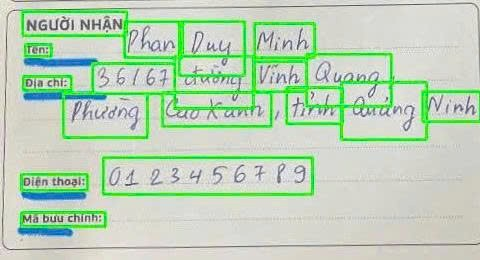
\includegraphics[width=\textwidth]{Images/fig4_7.jpg}
\caption{Text regions detected with EasyOCR.}
\label{fig:easyocrregions}
\end{figure}

\begin{table}[htbp]
\centering
\caption{Example of the layout reconstruction process}
\label{tab:layoutexample}
\small
\begin{tabular}{ll}
\hline
\textbf{Stage} & \textbf{Content} \\
\hline
Fragmented text regions & ``Tên''; ``Phan''; ``Duy''; ``Minh'' \\
After MERGE & ``Tên''; ``Phan Duy Minh'' \\
After PAIR & Label ``Tên'' paired with value ``Phan Duy Minh'' \\
\hline
\end{tabular}
\end{table}

\textbf{Raw text assembly.} Once the logical table has been built, the cells of each row are joined in the correct column order to form a line of text, and the lines are then concatenated with newline characters to produce the complete raw text for each area. For example, if a row has the label ``Họ và tên'' and the value ``John Doe'', the corresponding line of raw text is ``Họ và tên John Doe''.

\textbf{Field extraction.} The raw text is passed to the Claude Sonnet 5 model, \texttt{claude-sonnet-5}, through the Claude API \cite{anthropic_sonnet5}, together with a prompt requesting the extraction of 11 fields: \texttt{sender\_\allowbreak name}, \texttt{sender\_\allowbreak phone}, \texttt{sender\_\allowbreak province}, \texttt{sender\_\allowbreak ward}, \texttt{sender\_\allowbreak address}, \texttt{receiver\_\allowbreak name}, \texttt{receiver\_\allowbreak phone}, \texttt{receiver\_\allowbreak province}, \texttt{receiver\_\allowbreak ward}, \texttt{receiver\_\allowbreak address} and \texttt{item\_\allowbreak description}. The result is returned in JSON format; fields that are not found are set to \texttt{null} and listed in \texttt{missing\_fields} so that the system can request them manually.

\subsection{Webcam-Based Dimension Measurement}

The webcam-based method proceeds as follows. YOLO26n detects the person region and YOLO Hand Keypoints detects hands and their keypoints; both regions are masked. YOLO Package Detection then determines the bounding box of the parcel, which is used to crop the region of interest. Canny edge detection identifies the boundaries within that region, the pixel dimensions are converted into centimetres, and the three dimensions are used to compute the volume.

The first camera is fixed in front of the parcel to determine its horizontal width and height. Because the distance between the camera and the measurement area does not change, each pixel is converted into a real length through a coefficient $K$, as given in Equation~\eqref{eq:pixel2cm}:

\begin{equation}
\label{eq:pixel2cm}
L = p_L \times K, \qquad H = p_H \times K
\end{equation}

where $p_L$ and $p_H$ are the numbers of pixels along the horizontal and vertical directions in the front camera image, $K$ is the conversion coefficient in centimetres per pixel, and $L$ and $H$ are the real horizontal width and height.

The second camera is placed above the parcel and observes both the horizontal width and the depth. Since the real width $L$ has already been determined from the first camera, the depth is derived from the ratio between the two dimensions in the top camera image, as given in Equation~\eqref{eq:depthratio}:

\begin{equation}
\label{eq:depthratio}
W = L \times \frac{p_W}{p'_L}
\end{equation}

where $p_W$ is the number of pixels along the depth direction, $p'_L$ is the number of pixels along the horizontal direction in the top camera image, and $W$ is the real depth of the parcel. Once the three dimensions have been determined, the volume is computed with Equation~\eqref{eq:volume} and sent to the web interface for price calculation.

\subsection{Ultrasonic-Sensor-Based Dimension Measurement}

The measurement algorithm is shown in Figure~\ref{fig:ultrasonicalgo}. First, the ESP32 reads the temperature from the \mbox{SHT30-D} sensor and computes the speed of sound with Equation~\eqref{eq:speedofsound}. The ESP32 then sends a 10-microsecond HIGH pulse in turn to the trigger pin of each ultrasonic sensor. Sequential triggering is used to limit cross-talk between the three sensors.

\begin{figure}[htbp]
\centering
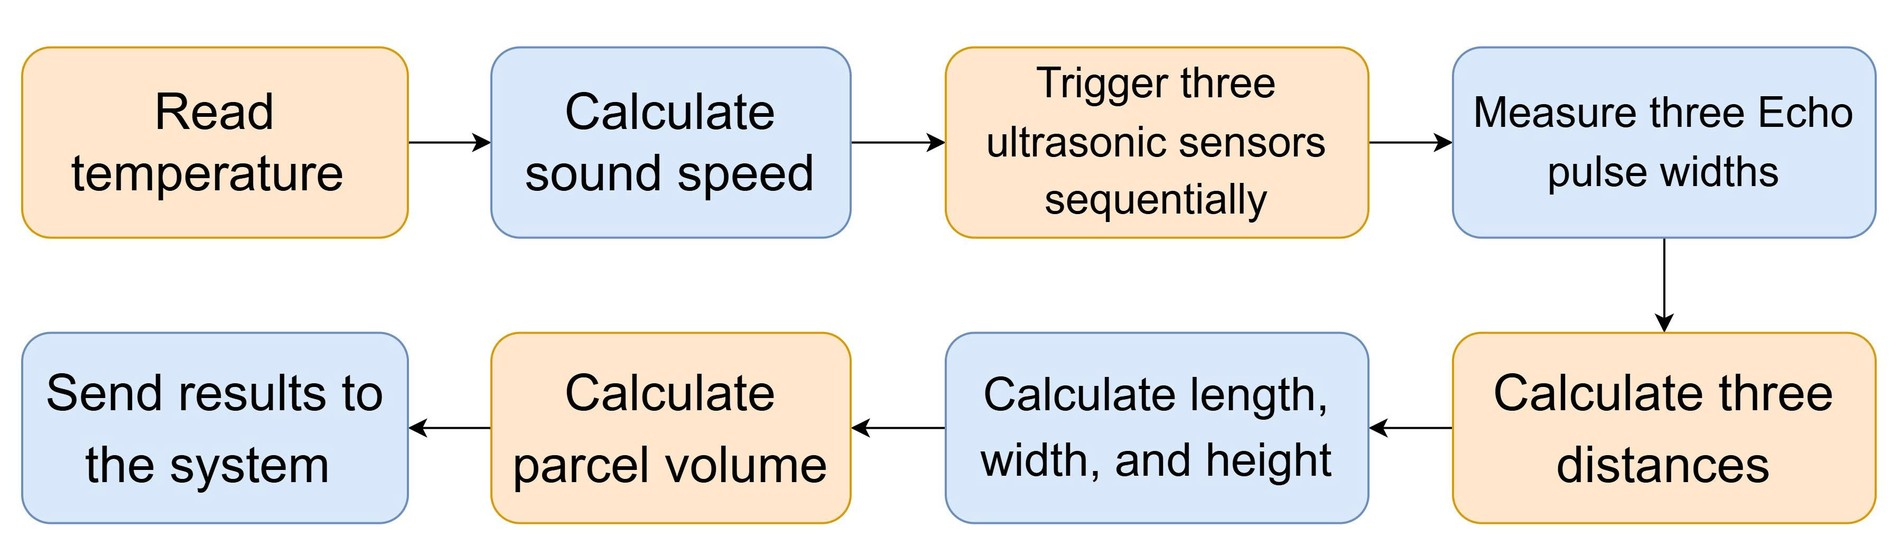
\includegraphics[width=\textwidth]{Images/fig4_8.jpg}
\caption{Algorithm for dimension and volume measurement with ultrasonic sensors.}
\label{fig:ultrasonicalgo}
\end{figure}

Once triggered, each sensor emits a 40\,kHz ultrasonic wave \cite{hcsr04, srf05} towards the parcel and receives the wave reflected from its surface. The ESP32 measures the width of the echo pulse to determine the round-trip travel time, and then computes the distance with Equation~\eqref{eq:tof} \cite{openstax_sound, hcsr04, srf05}. From the three distances obtained, the system determines the parcel dimensions with Equations~\eqref{eq:usL} to \eqref{eq:usH}:

\begin{align}
L &= 105 - d_1 \label{eq:usL}\\
W &= 105 - d_2 \label{eq:usW}\\
H &= 105 - d_3 \label{eq:usH}
\end{align}

\indent where $d_1$, $d_2$ and $d_3$ are the distances from the three sensors to the parcel surface, and $L$, $W$ and $H$ are respectively the length, width and height of the parcel in centimetres. The parcel volume is computed with Equation~\eqref{eq:volume} and sent to the web interface for price calculation.

\subsection{Shipping Fee Calculation}

The fee calculation pipeline, shown in Figure~\ref{fig:feepipeline}, takes as input the service, the origin, the destination, the actual weight and the parcel dimensions. The service codes, route groups, weight tiers and unit prices used in the module were built from the business knowledge base and the 2026 tariff table provided by the post office \cite{vnpost_kb2026, vnpost_tariff2026} (see Appendices~A and~B).

\begin{figure}[htbp]
\centering
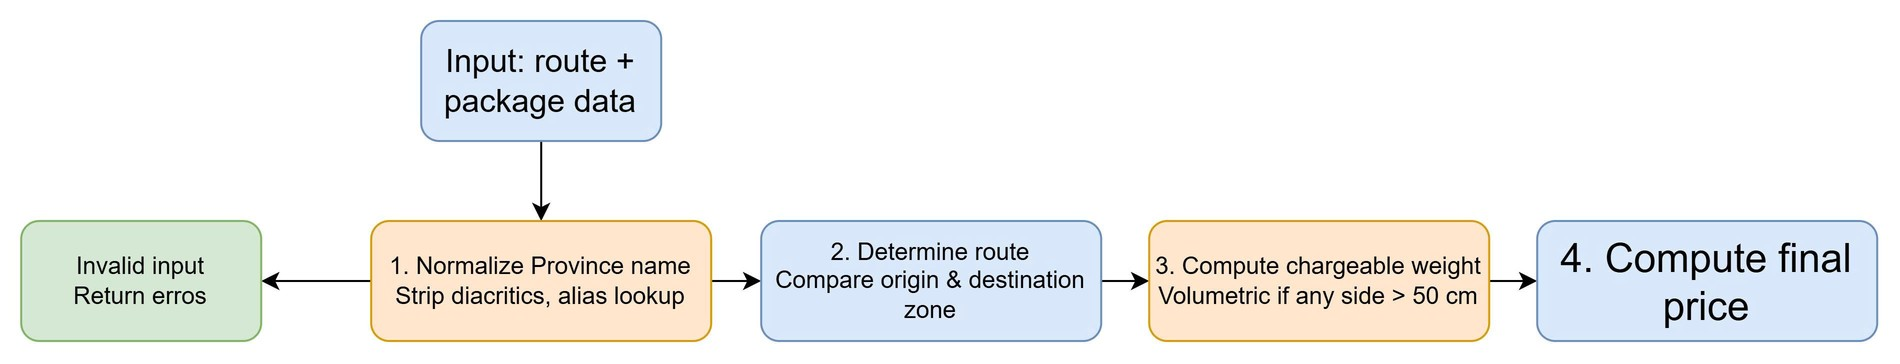
\includegraphics[width=\textwidth]{Images/fig4_9.jpg}
\caption{Shipping fee calculation pipeline.}
\label{fig:feepipeline}
\end{figure}

The calculation consists of four steps.

\textbf{Step 1: province normalization.} The key \texttt{key(province\_input)} is computed by stripping diacritics, lowercasing, and keeping only letters and digits. The alias table is looked up first; if there is no match, the province table \texttt{\_province\_map} is looked up directly; if there is still no match, an invalid-province error is raised. For example, ``Hà nội'' maps to the key \texttt{hanoi} and then to ``Hà Nội'', while ``TP HCM'' maps to \texttt{tphochiminh} and then to ``TP. Hồ Chí Minh''.

\textbf{Step 2: route determination.} The origin and destination are normalized to their canonical names and the zone of each is looked up. If the origin equals the destination the route is intra-province; if both lie in the same zone the route is intra-zone. If the zones differ, then for the ETN service group, covering ETN001, ETN011 and ETN013, the Hà Nội--TP.HCM pair and routes involving Đà Nẵng are assigned to special routes while the rest are inter-zone; for the CTN001 service, the route is near-zone if either end lies in Zone 3 and far-zone otherwise. This division is configured according to the corresponding business documentation and tariff table structure \cite{vnpost_kb2026, vnpost_tariff2026} (see Appendices~A and~B).

\textbf{Step 3: chargeable weight computation.} The volumetric weight is computed as \texttt{weight\_volumetric} $= (L \times W \times H)/6000$. According to the business guidance provided by post office staff, within the scope of this experimental module the volumetric weight is considered when at least one edge of the parcel exceeds 50\,cm; in that case the chargeable weight is the larger of the actual weight and the volumetric weight \cite{vnpost_kb2026} (see Appendix~A). If no edge exceeds 50\,cm, the system uses the actual weight.

\textbf{Step 4: final price computation.} The \texttt{route\_index} corresponding to the route and service is looked up. For CTN001, \texttt{base\_tiers} gives the base price and the base threshold \texttt{base\_limit}; if the weight exceeds the threshold, the cost of each tier in \texttt{progressive\_tiers} into which the excess weight falls is accumulated. For the ETN group, \texttt{base\_tiers} gives the base price and the threshold; if the threshold is exceeded, a surcharge equal to the number of excess units \texttt{unit\_grams} multiplied by the surcharge unit price of the corresponding route is added. The module returns a result object containing the service, the route, the actual weight, the chargeable weight, a flag indicating whether the volumetric weight was used, and the final amount. The base price, the next weight unit and the unit price of the excess portion for each service are taken from the 2026 tariff table \cite{vnpost_tariff2026} (see Appendix~B).

The main parameters of the module are listed in Table~\ref{tab:feeparams}.

\begin{table}[htbp]
\centering
\caption{Main parameters of the fee calculation module}
\label{tab:feeparams}
\small
\begin{tabular}{R{6.2cm}R{7.0cm}}
\hline
\textbf{Parameter} & \textbf{Value or meaning} \\
\hline
Volumetric conversion factor & 6000, following the industry standard $(L \times W \times H)/6000$ in kilograms \\
Threshold for applying volumetric weight & longest edge greater than 50\,cm \\
Surcharge rounding unit for ETN services & \texttt{unit\_grams}, for example 500\,g \\
Number of supported services & 5: LETTER, ETN001, ETN011, ETN013, CTN001 \\
\hline
\end{tabular}
\end{table}

\section{Hyperparameter and Training Setup}
\label{sec:training}

\subsection{Data Splitting Strategy}

The split applied to each model is shown in Table~\ref{tab:datasplit}.

\begin{table}[htbp]
\centering
\caption{Data splits for the models used in this project}
\label{tab:datasplit}
\small
\begin{tabular}{R{3.6cm}R{3.8cm}rrr}
\hline
\textbf{Model} & \textbf{Dataset} & \textbf{Train} & \textbf{Val.} & \textbf{Test} \\
\hline
Box/Envelope Detection & Postal Item Dataset & 1,050 & 44 & 44 \\
Information Region Detection & Postal Item Dataset & 503 & 22 & 22 \\
TrOCR & Viet-\hspace{0pt}Handwriting-\hspace{0pt}OCR-v2 & 58,247 & 1,000 & 1,000 \\
YOLO Package Detection & Cardboard Box Detection & 7,373 & 922 & 921 \\
YOLO Hand Keypoints & Hand Keypoints Dataset & 18,776 & 3,996 & 3,996 \\
\hline
\end{tabular}
\end{table}

For Box/Envelope Detection, the training set was augmented from 351 to 1,050 images, while the validation and testing sets were kept unchanged at 44 images each. For Information Region Detection, only images containing parcels were selected; after cropping the parcel region and converting the coordinates of the \texttt{Label\_info} class, the dataset consists of 503 training images, 22 validation images and 22 testing images.

Viet-Handwriting-OCR-v2 originally consists of 59,247 training samples and 1,000 testing samples. The team used \texttt{train\_test\_split} with \texttt{test\_size = 1000} and \texttt{seed = 42} to separate 1,000 samples from the training set as a validation set. The remaining 58,247 samples were used for training, and the original testing set was kept unchanged for the final evaluation. The fixed seed makes this split reproducible.

YOLO26n Person Detection uses pretrained weights and was not retrained on the project data, so it does not appear in Table~\ref{tab:datasplit}.

\subsection{YOLO11n Training Configuration}

After preprocessing, a new dataset was generated automatically for fine-tuning a second YOLO11n. Information Region Detection has the single task of locating the information label region within the cropped box image, and was trained with parameters similar to Box/Envelope Detection. The configuration is given in Table~\ref{tab:yolocfg}. After training, the best weights of Information Region Detection were saved in the \texttt{weights/best.pt} directory.

\begin{table}[htbp]
\centering
\caption{Training configuration of the two YOLO11n models}
\label{tab:yolocfg}
\small
\begin{tabular}{lll}
\hline
\textbf{Parameter} & \textbf{Box/Envelope Detection} & \textbf{Information Region Detection} \\
\hline
Model & YOLO11n & YOLO11n \\
Pretrained weights & \texttt{yolo11n.pt} & \texttt{yolo11n.pt} \\
Number of classes & 2 & 1 \\
Classes & \texttt{Label\_Box}, \texttt{Label\_Envelope} & \texttt{Label\_info} \\
Epochs & 50 & 50 \\
Image size & $640 \times 640$ & $640 \times 640$ \\
Batch size & 16 & 16 \\
Device & 0 (GPU 0) & 0 (GPU 0) \\
Workers & 4 & 4 \\
\hline
\end{tabular}
\end{table}

\subsection{TrOCR Training Configuration}

The TrOCR fine-tuning process loads the \texttt{microsoft/trocr-base-handwritten} checkpoint, prepares the data with a custom \texttt{TrOCRDataset}, assigns $-100$ to padding tokens so that these positions do not contribute to the loss, freezes the entire encoder and fine-tunes only the decoder. Training is performed with \texttt{Seq2SeqTrainer}, which evaluates and saves a checkpoint every 1,000 steps. The checkpoint with the lowest \texttt{eval\_loss} is selected, and inference is then run on the test set to compute the character error rate and the word error rate with the \texttt{jiwer} library. The configuration is given in Table~\ref{tab:trocrcfg}.

\begin{table}[htbp]
\centering
\caption{TrOCR fine-tuning configuration}
\label{tab:trocrcfg}
\small
\begin{tabular}{R{6.2cm}R{7.0cm}}
\hline
\textbf{Parameter} & \textbf{Value} \\
\hline
Number of epochs & 3 \\
Batch size per device & 2 \\
Gradient accumulation & 4, giving an effective batch size of 8 \\
Learning rate & $1 \times 10^{-5}$ \\
Warmup ratio & 0.1 \\
Optimizer & AdamW, the \texttt{Seq2SeqTrainer} default \\
Regularization & Gradient checkpointing, fp16 mixed precision \\
Evaluation and save steps & Every 1,000 steps, keeping at most 2 checkpoints \\
Best-model selection criterion & Lowest \texttt{eval\_loss}, using \texttt{load\_best\_model\_at\_end} \\
\hline
\end{tabular}
\end{table}

\subsection{Webcam Model Training Configuration}

The webcam system uses one pretrained person detection model and two models fine-tuned for hand detection and parcel detection, on the splits given in Table~\ref{tab:datasplit}. The hyperparameters were kept identical for the two fine-tuning runs, as listed in Table~\ref{tab:hyperparams}.

\begin{table}[htbp]
\centering
\caption{Training parameters used for the webcam system models}
\label{tab:hyperparams}
\small
\begin{tabular}{R{6.2cm}R{7.0cm}}
\hline
\textbf{Hyperparameter} & \textbf{Value} \\
\hline
Number of epochs & 100 \\
Input image size (\texttt{imgsz}) & $640 \times 640$ \\
Batch size & 16 \\
Training device (\texttt{device}) & GPU 0 \\
Number of data loading workers (\texttt{workers}) & 0 \\
\hline
\end{tabular}
\end{table}

Training was carried out on an NVIDIA GeForce RTX 3050 GPU with 4\,GB of VRAM. An image size of $640 \times 640$ was used to standardize the model input. The batch size was set to 16 to fit within the GPU memory limit, while 100 epochs allowed the model to update its weights over many passes through the data. For the webcam-system models, \texttt{workers = 0} was used as a conservative configuration so that data loading was performed in the main process. This setting was specific to these training runs and does not imply that Windows is incompatible with multiprocessing. The two YOLO11n models reported in Table~\ref{tab:yolocfg} were successfully trained with \texttt{workers = 4} on the same machine. YOLO26n Person Detection uses pretrained weights and was not retrained on the project data, so it does not appear in the training configuration.

\chapter{Results Analysis}
\label{chap:results}

This chapter reports the experimental results of the system described in Chapter~\ref{chap:methodology} on the data described in Chapter~\ref{chap:data_processing}. It begins with the experimental setup, then presents the quantitative and qualitative results, and closes with an analysis of the observed errors.

\section{Experimental Setup}

All software components were run on a computer with an NVIDIA GeForce RTX 3050 GPU with 4\,GB of VRAM, using the Python implementation described in Chapter~\ref{chap:methodology}. The detection and recognition models were evaluated on the test splits given in Table~\ref{tab:datasplit}. Each of the two measurement subsystems was evaluated on its own physical setup, described below.

\subsection{Webcam-Based Measurement Setup}

The webcam dimension measurement experiment combines YOLO models and the OpenCV library to detect people, hands, parcels, edges and dimensions. The physical arrangement is shown in Figure~\ref{fig:webcamsetup}. The first camera is placed in front to capture the horizontal width and the height of the parcel, and the second camera is placed above to determine the ratio between the horizontal width and the depth. The images from both cameras are streamed directly to the computer.

\begin{figure}[htbp]
\centering
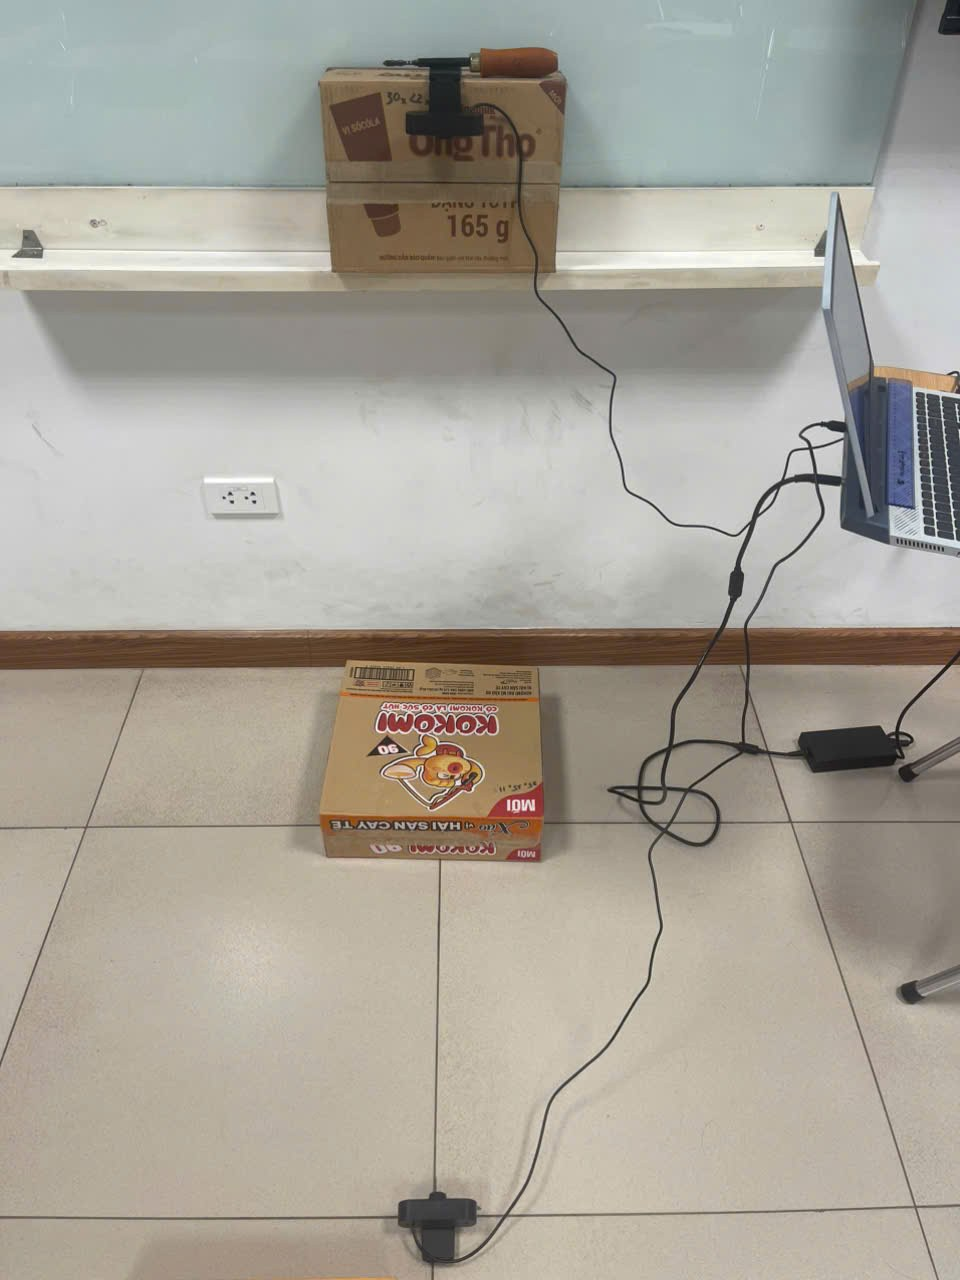
\includegraphics[width=0.72\textwidth]{Images/fig5_1.jpg}
\caption{Setup of the two-USB-camera dimension measurement system.}
\label{fig:webcamsetup}
\end{figure}

\subsection{Ultrasonic-Sensor Measurement Setup}

The ultrasonic measurement system consists of one ESP32, one HC-SRF05 sensor, two HC-SR04 sensors and one \mbox{SHT30-D} temperature sensor. The wiring is shown in Figure~\ref{fig:ultrasonicwiring}. The first sensor uses GPIO27 and GPIO26; the second uses GPIO25 and GPIO34; the third uses GPIO32 and GPIO35, for the trigger and echo pins respectively. The \mbox{SHT30-D} is connected to the ESP32 through GPIO21 and GPIO22 over I\textsuperscript{2}C. The devices share a common power supply and ground on the breadboard, while the ESP32 is powered over USB at 5\,V.

\begin{figure}[htbp]
\centering
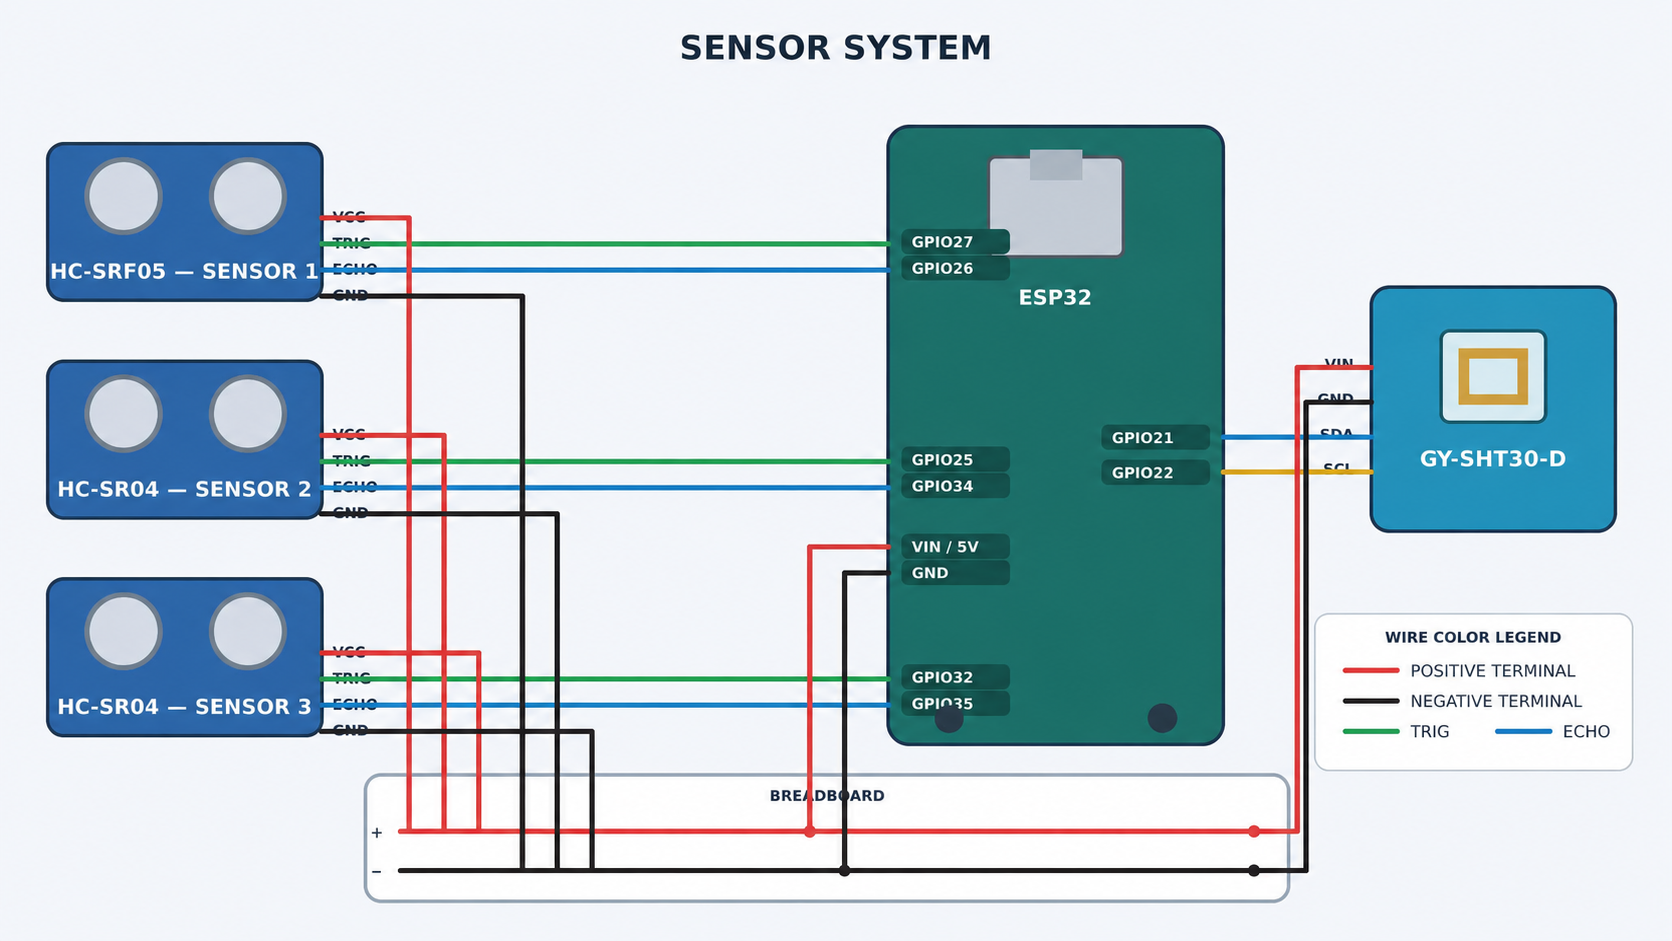
\includegraphics[width=0.82\textwidth]{Images/fig5_2.png}
\caption{Wiring diagram of the ultrasonic sensor system.}
\label{fig:ultrasonicwiring}
\end{figure}

The physical setup is shown in Figure~\ref{fig:ultrasonicreal}. The three sensors are fixed along three perpendicular axes to measure the length, width and height, with the parcel placed in the corner at the centre of the floor.

\begin{figure}[htbp]
\centering
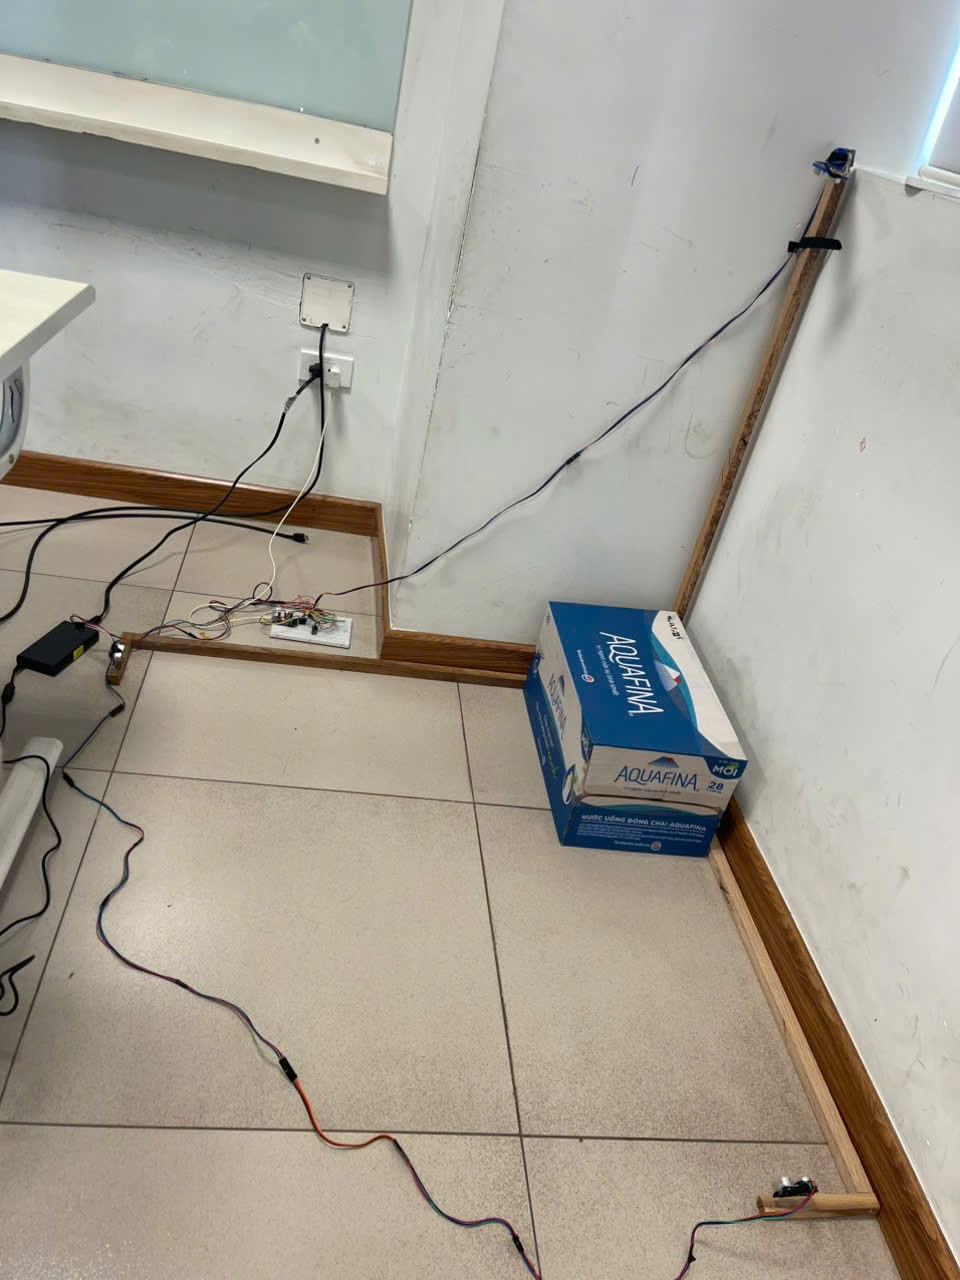
\includegraphics[width=0.72\textwidth]{Images/fig5_3.jpg}
\caption{Physical setup of the ultrasonic sensor system.}
\label{fig:ultrasonicreal}
\end{figure}

\section{Quantitative Results}
\label{sec:quantitative}

\subsection{Box/Envelope Detection}

Over 50 epochs, the training box loss decreased from 0.747 to 0.250, the classification loss from 2.017 to 0.169, and the distribution focal loss from 1.301 to 0.922. On the validation set, the box loss decreased from 1.517 to 0.237 and the classification loss from 2.484 to 0.167. The corresponding curves are shown in Figure~\ref{fig:boxloss}. The downward trend indicates that the model gradually learned the features needed both for localization and for distinguishing the two classes.

\begin{figure}[htbp]
\centering
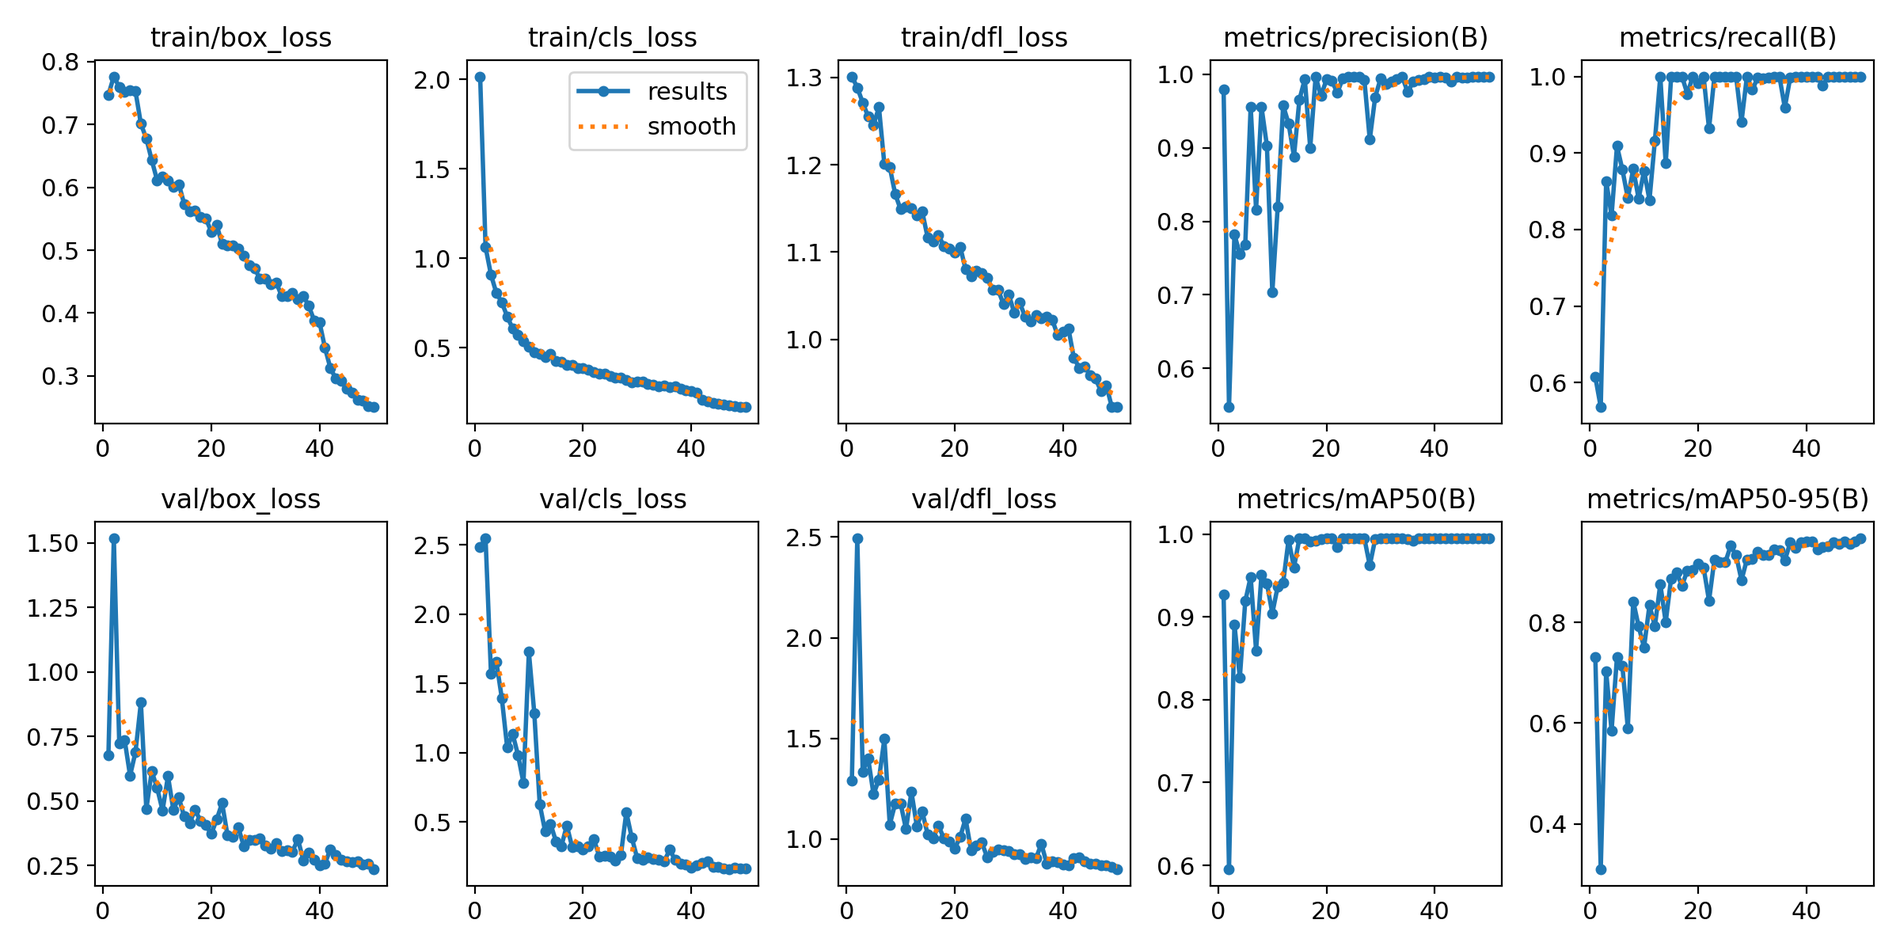
\includegraphics[width=\textwidth]{Images/fig5_4.png}
\caption{Loss and evaluation metrics of Box/Envelope Detection.}
\label{fig:boxloss}
\end{figure}

The results at the final epoch are given in Table~\ref{tab:boxenvres}. The model detects most objects correctly and misses only a very small proportion on the evaluation set. The relatively small gap between mAP@50 and mAP@50--95 indicates that the model maintains a high score even when bounding box localization is required to be more precise.

\begin{table}[htbp]
\centering
\caption{Quantitative results of Box/Envelope Detection}
\label{tab:boxenvres}
\small
\begin{tabular}{cccc}
\hline
\textbf{Precision} & \textbf{Recall} & \textbf{mAP@50} & \textbf{mAP@50--95} \\
\hline
0.9965 & 0.9972 & 0.9950 & 0.9666 \\
\hline
\end{tabular}
\end{table}

The per-class precision--recall curve in Figure~\ref{fig:boxpr} shows balanced performance across the two categories: both Label-Box and Label-envelope reach an average precision of 0.995 at an intersection over union threshold of 0.5.

\begin{figure}[htbp]
\centering
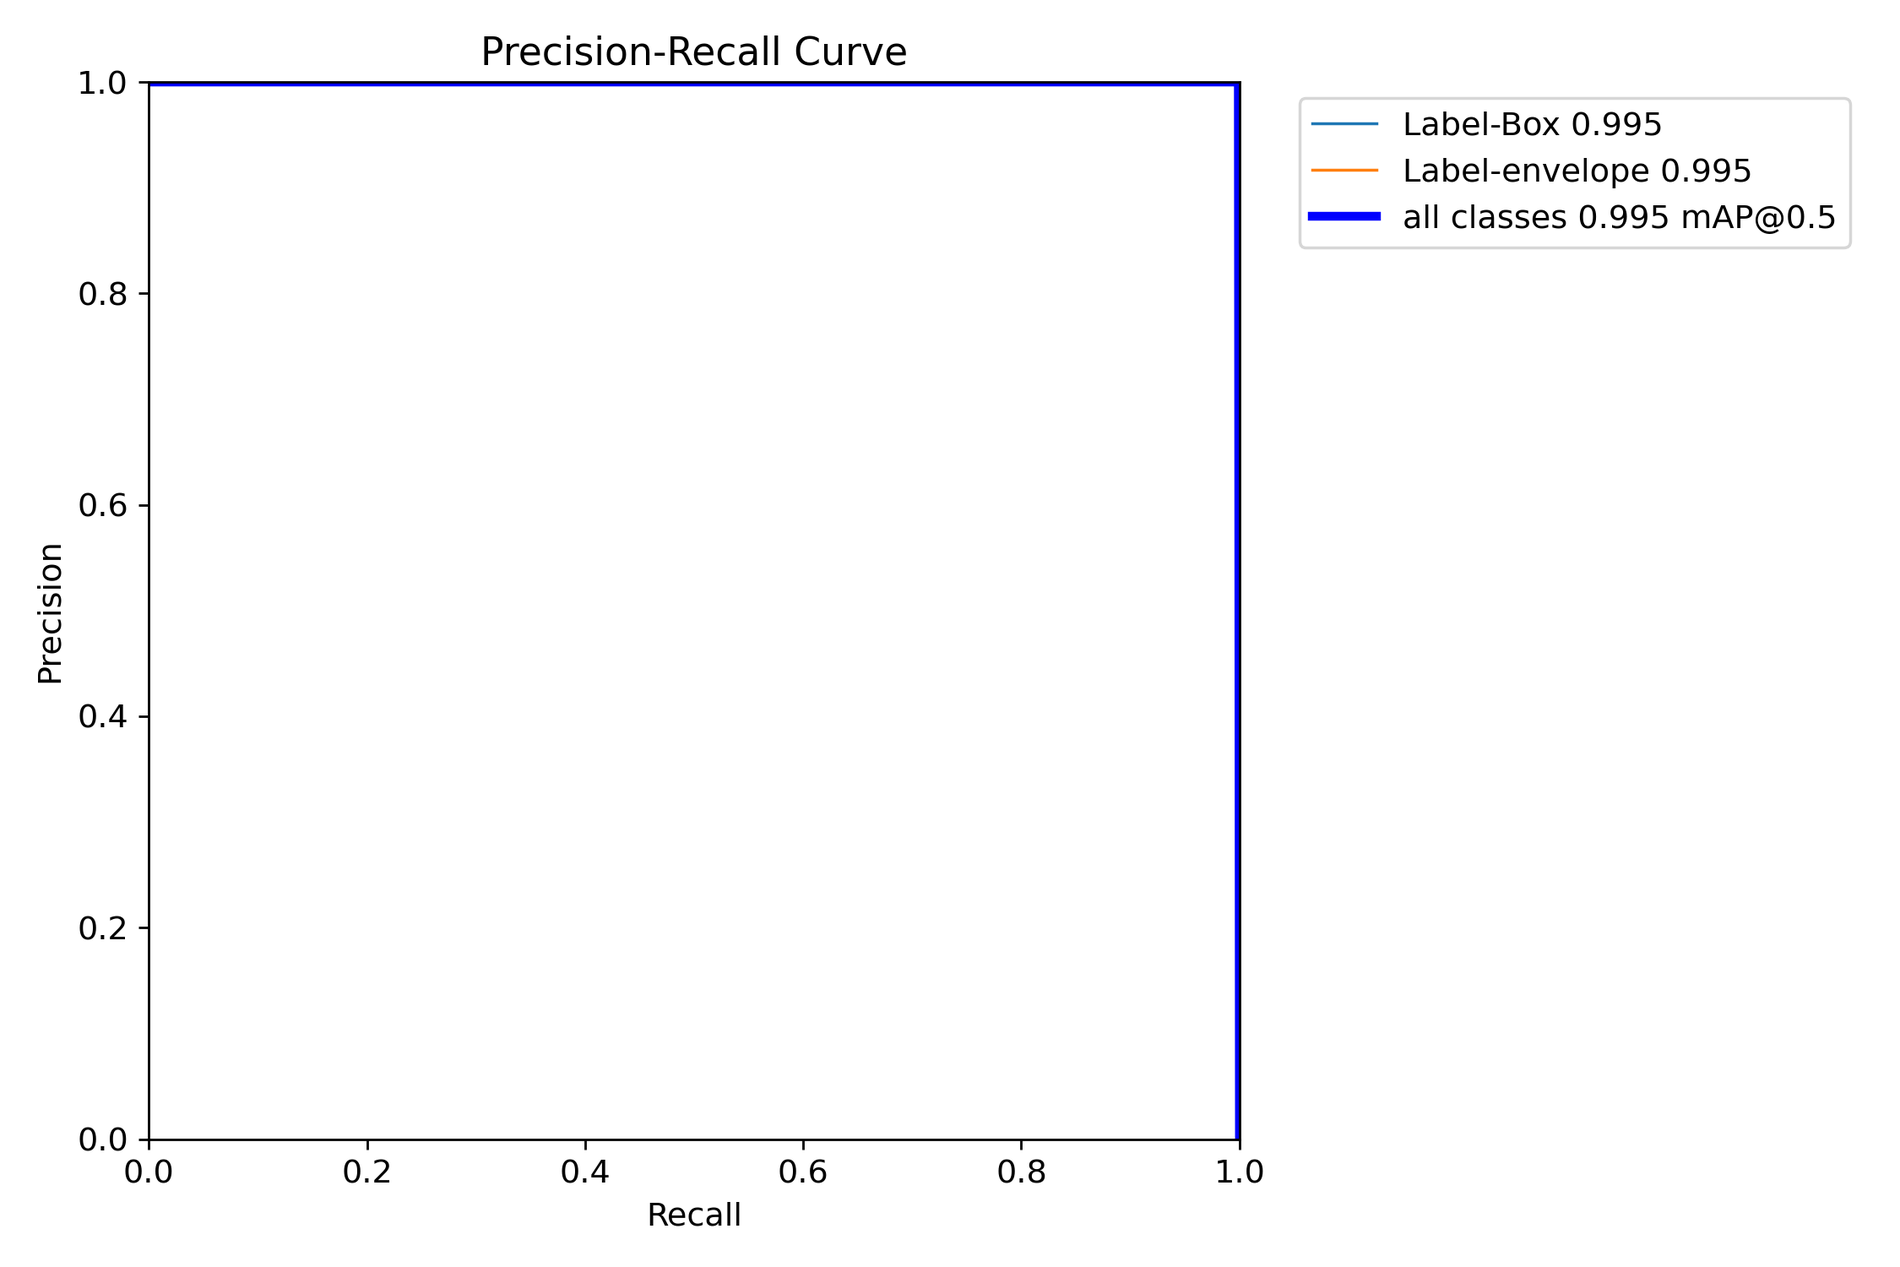
\includegraphics[width=0.78\textwidth]{Images/fig5_5.png}
\caption{Precision--recall curve of Box/Envelope Detection.}
\label{fig:boxpr}
\end{figure}

The confusion matrix in Figure~\ref{fig:boxcm} records 22 \texttt{Label\_Box} samples and 22 \texttt{Label\_Envelope} samples predicted correctly, with no case of misclassification between the two classes in the evaluation set.

\begin{figure}[htbp]
\centering
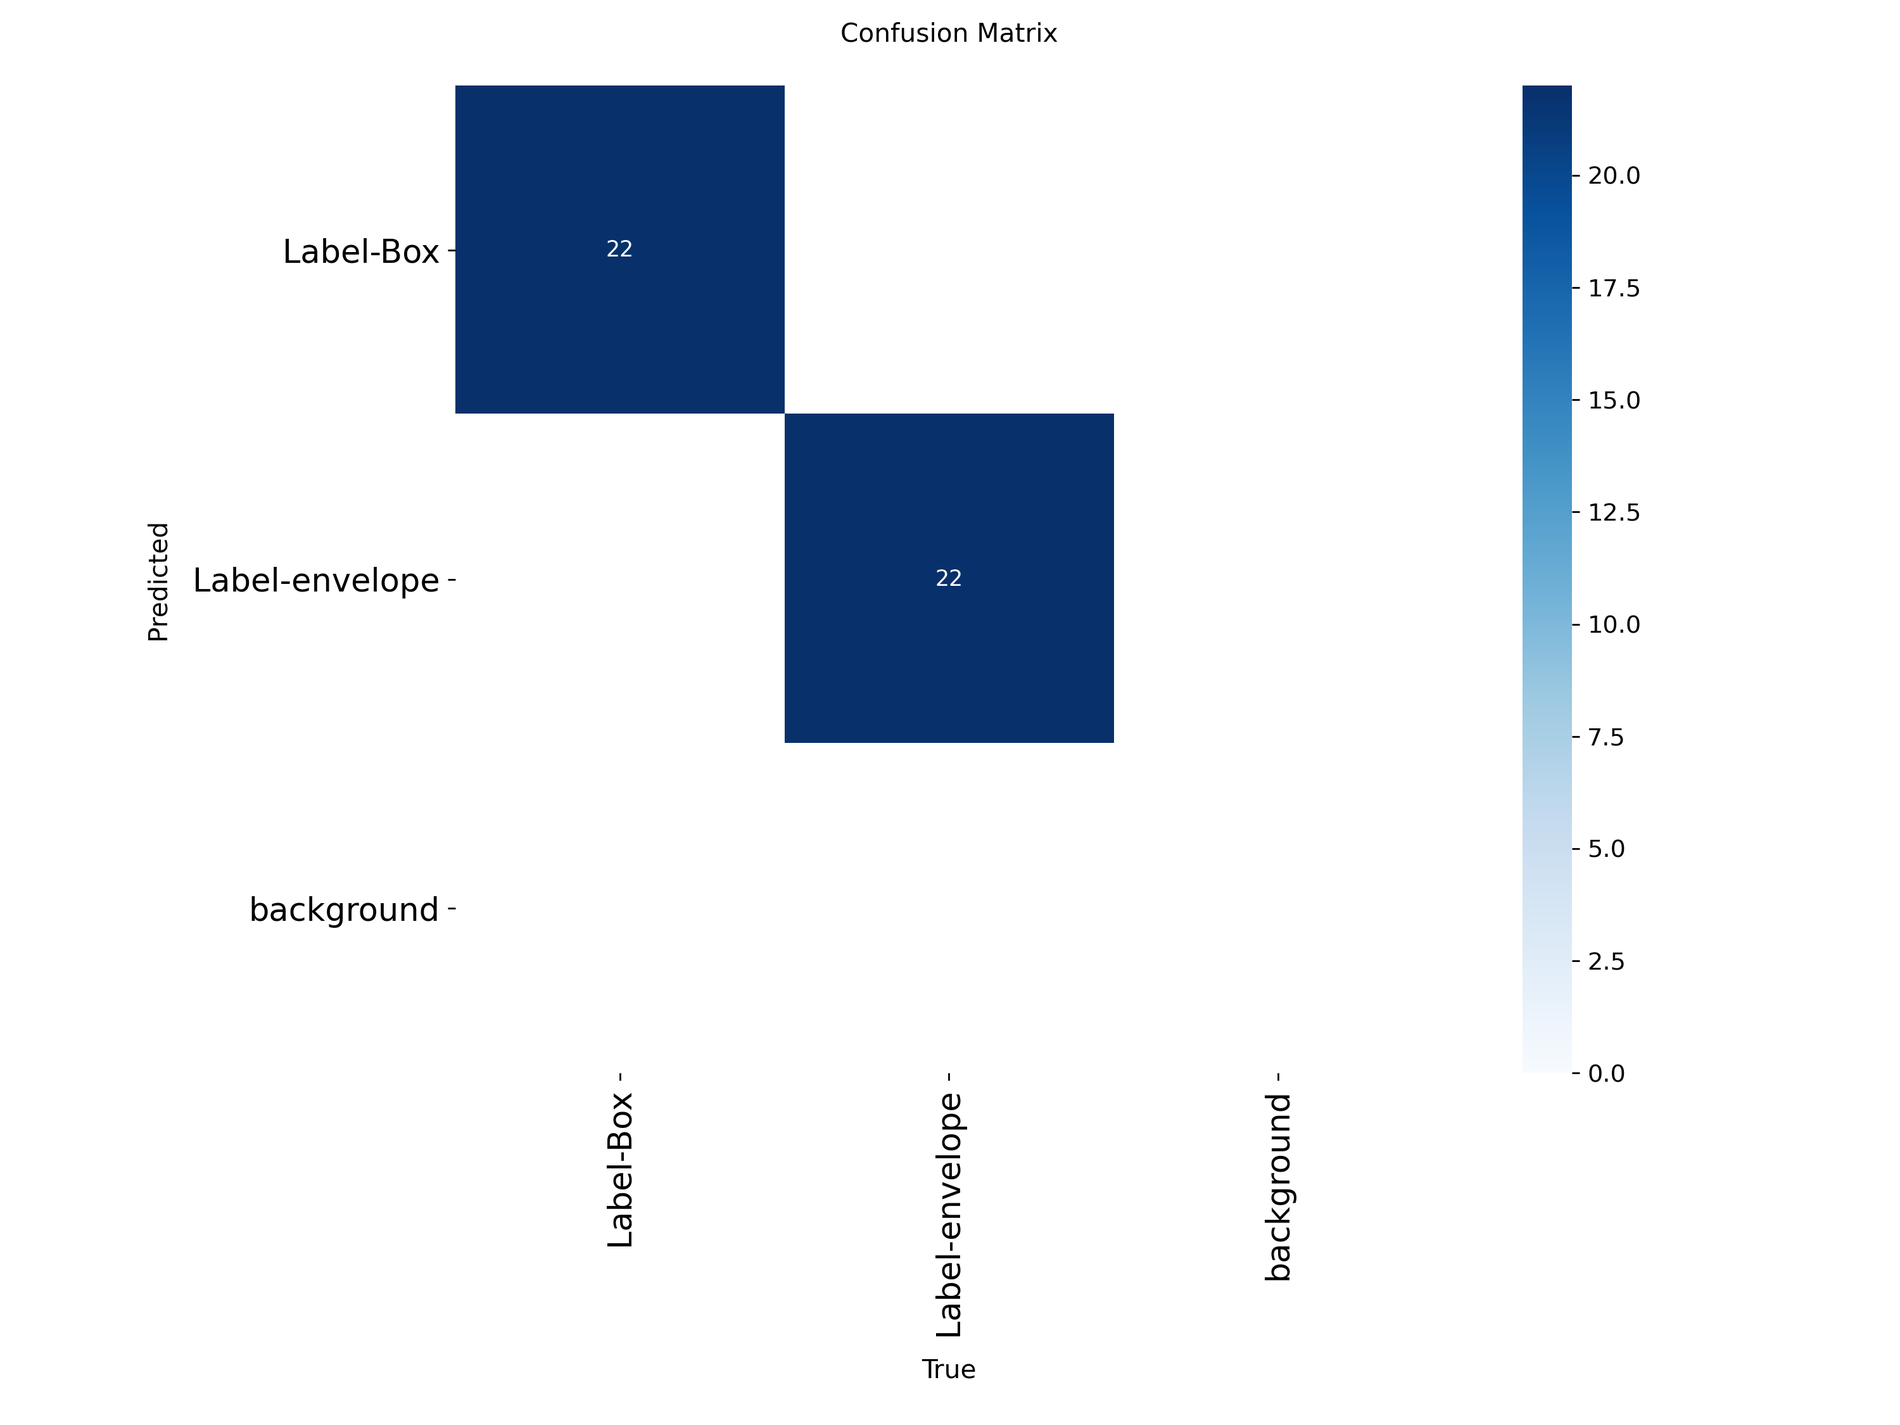
\includegraphics[width=0.78\textwidth]{Images/fig5_6.png}
\caption{Confusion matrix of Box/Envelope Detection.}
\label{fig:boxcm}
\end{figure}

As shown in Figure~\ref{fig:boxf1}, the F1 score reaches its maximum value of 1.00 at a confidence threshold of about 0.851 on the evaluation set.

\begin{figure}[htbp]
\centering
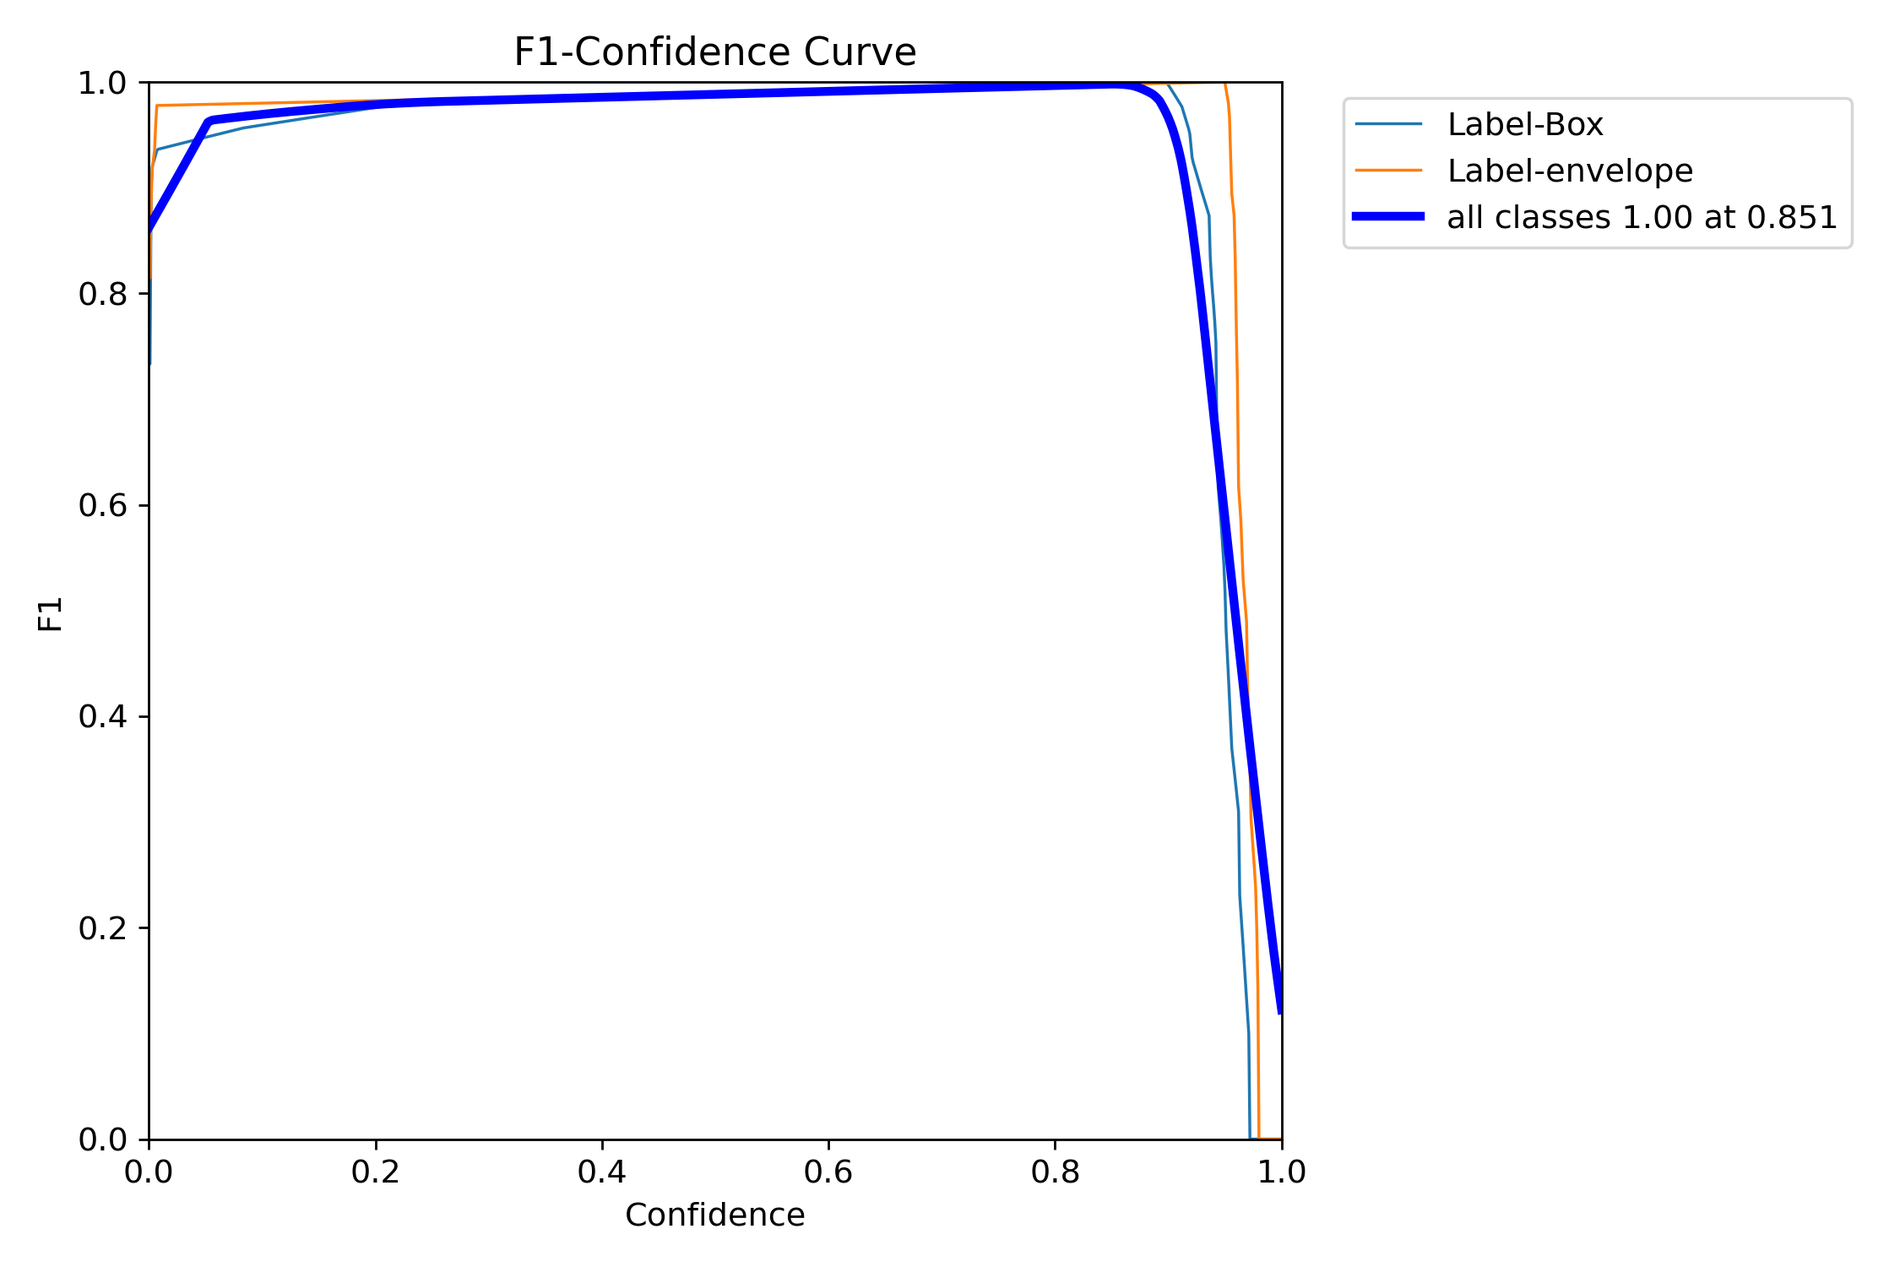
\includegraphics[width=0.78\textwidth]{Images/fig5_7.png}
\caption{F1--confidence curve of Box/Envelope Detection.}
\label{fig:boxf1}
\end{figure}

\subsection{Information Region Detection}

Over 50 epochs, the training box loss decreased from 0.8956 to 0.4692, the classification loss from 2.0926 to 0.2563, and the distribution focal loss from 1.3531 to 1.0279. On the validation set, the box loss decreased from 0.8815 to 0.4392 and the classification loss from 3.1052 to 0.3642. The curves are shown in Figure~\ref{fig:infoloss}. Although the results fluctuate over the first few epochs, the loss values generally decrease throughout training.

\begin{figure}[htbp]
\centering
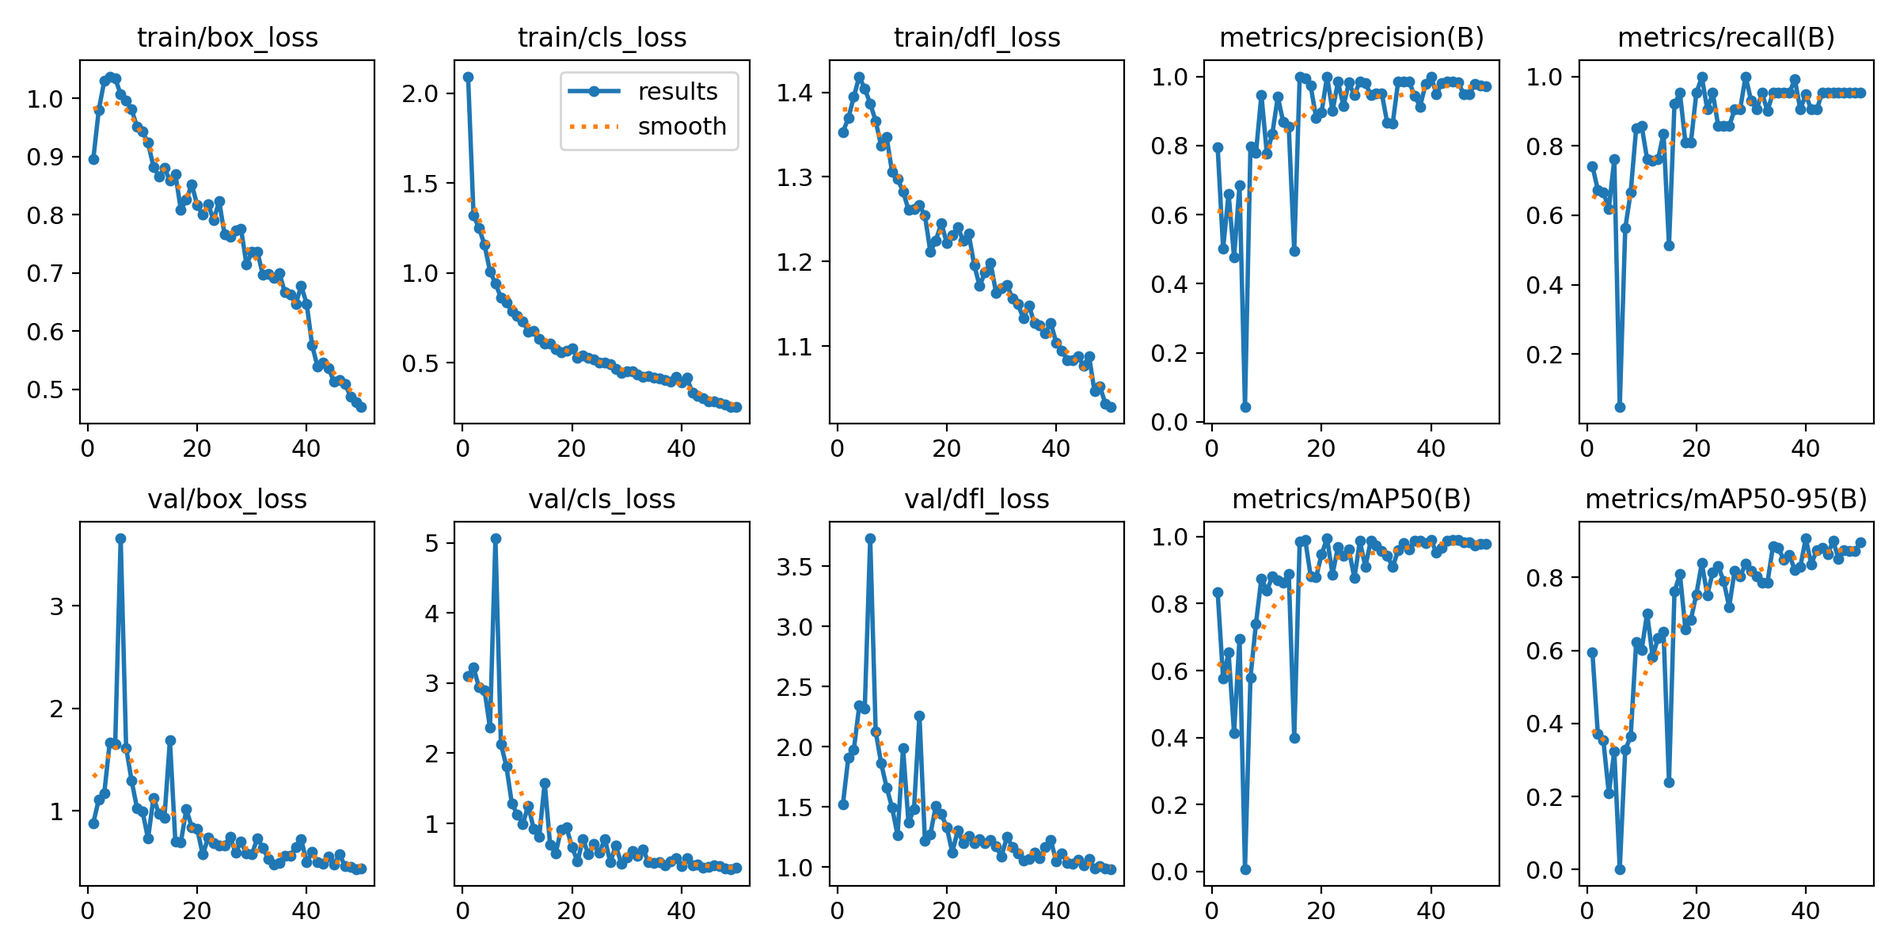
\includegraphics[width=\textwidth]{Images/fig5_8.png}
\caption{Loss and evaluation metrics of Information Region Detection.}
\label{fig:infoloss}
\end{figure}

The results at epoch 50 are given in Table~\ref{tab:infores}. During training, mAP@50 reached its highest value of 99.50\% at epoch 21, while mAP@50--95 reached its highest value of 90.67\% at epoch 40. The lower result for mAP@50--95 indicates that bounding box accuracy decreases at stricter intersection over union thresholds.

\begin{table}[htbp]
\centering
\caption{Quantitative results of Information Region Detection}
\label{tab:infores}
\small
\begin{tabular}{cccc}
\hline
\textbf{Precision} & \textbf{Recall} & \textbf{mAP@50} & \textbf{mAP@50--95} \\
\hline
97.15\% & 95.24\% & 97.90\% & 89.55\% \\
\hline
\end{tabular}
\end{table}

The confusion matrix in Figure~\ref{fig:infocm} shows that 21 Label-info samples were detected correctly, while 2 background samples were misclassified as Label-info. No significant number of Label-info objects was missed in this evaluation. This indicates that the second model recognizes the target class well, with only a few false-positive detections.

\begin{figure}[htbp]
\centering
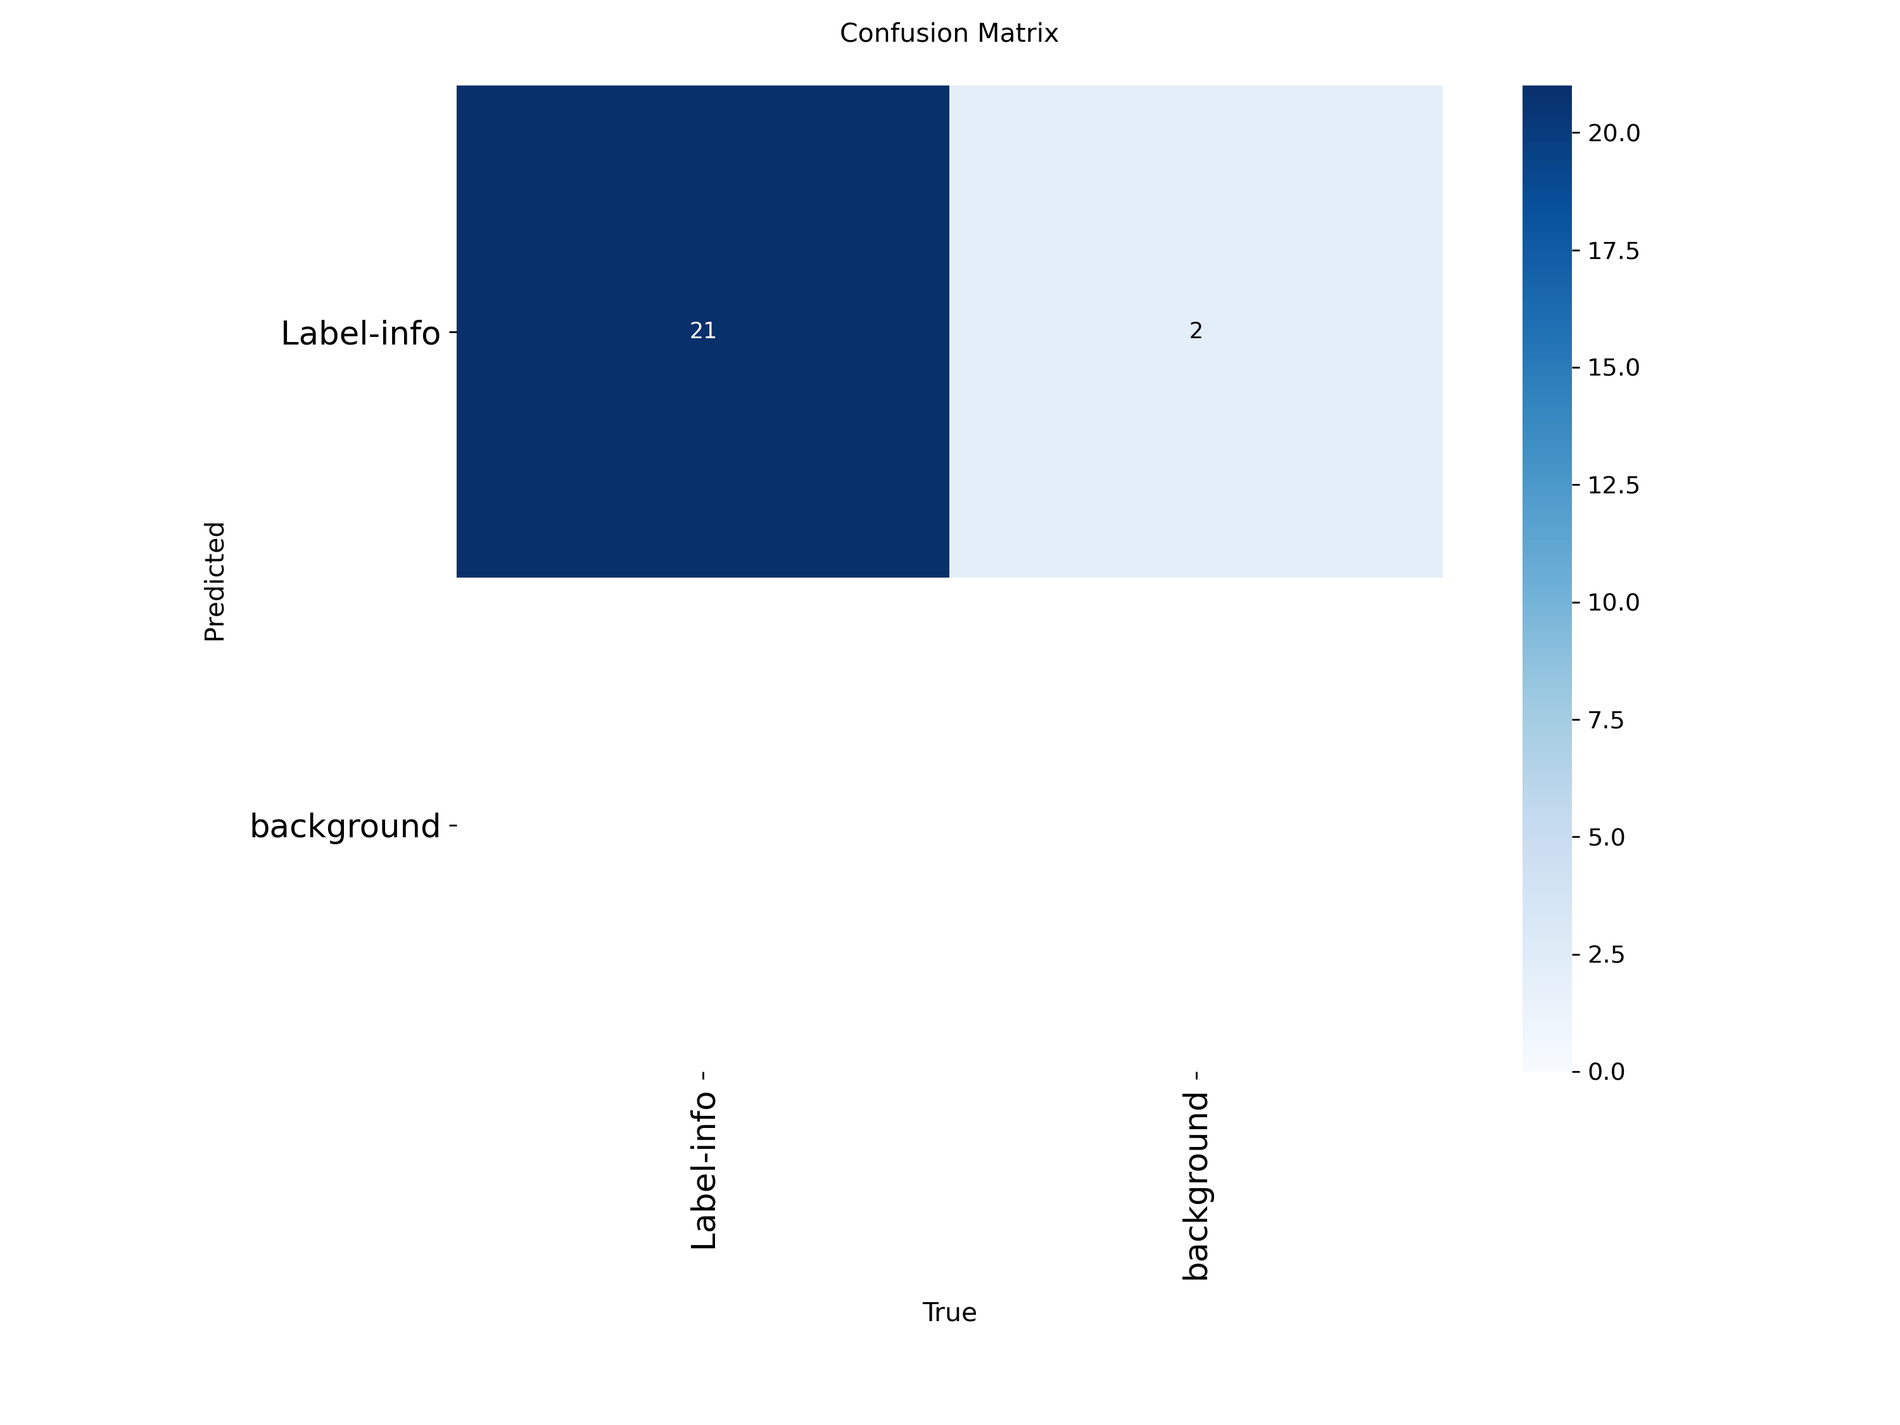
\includegraphics[width=0.78\textwidth]{Images/fig5_9.png}
\caption{Confusion matrix of Information Region Detection.}
\label{fig:infocm}
\end{figure}

The area under the precision--recall curve in Figure~\ref{fig:infopr} is about 0.992, showing that the model maintains high precision over a wide recall range.

\begin{figure}[htbp]
\centering
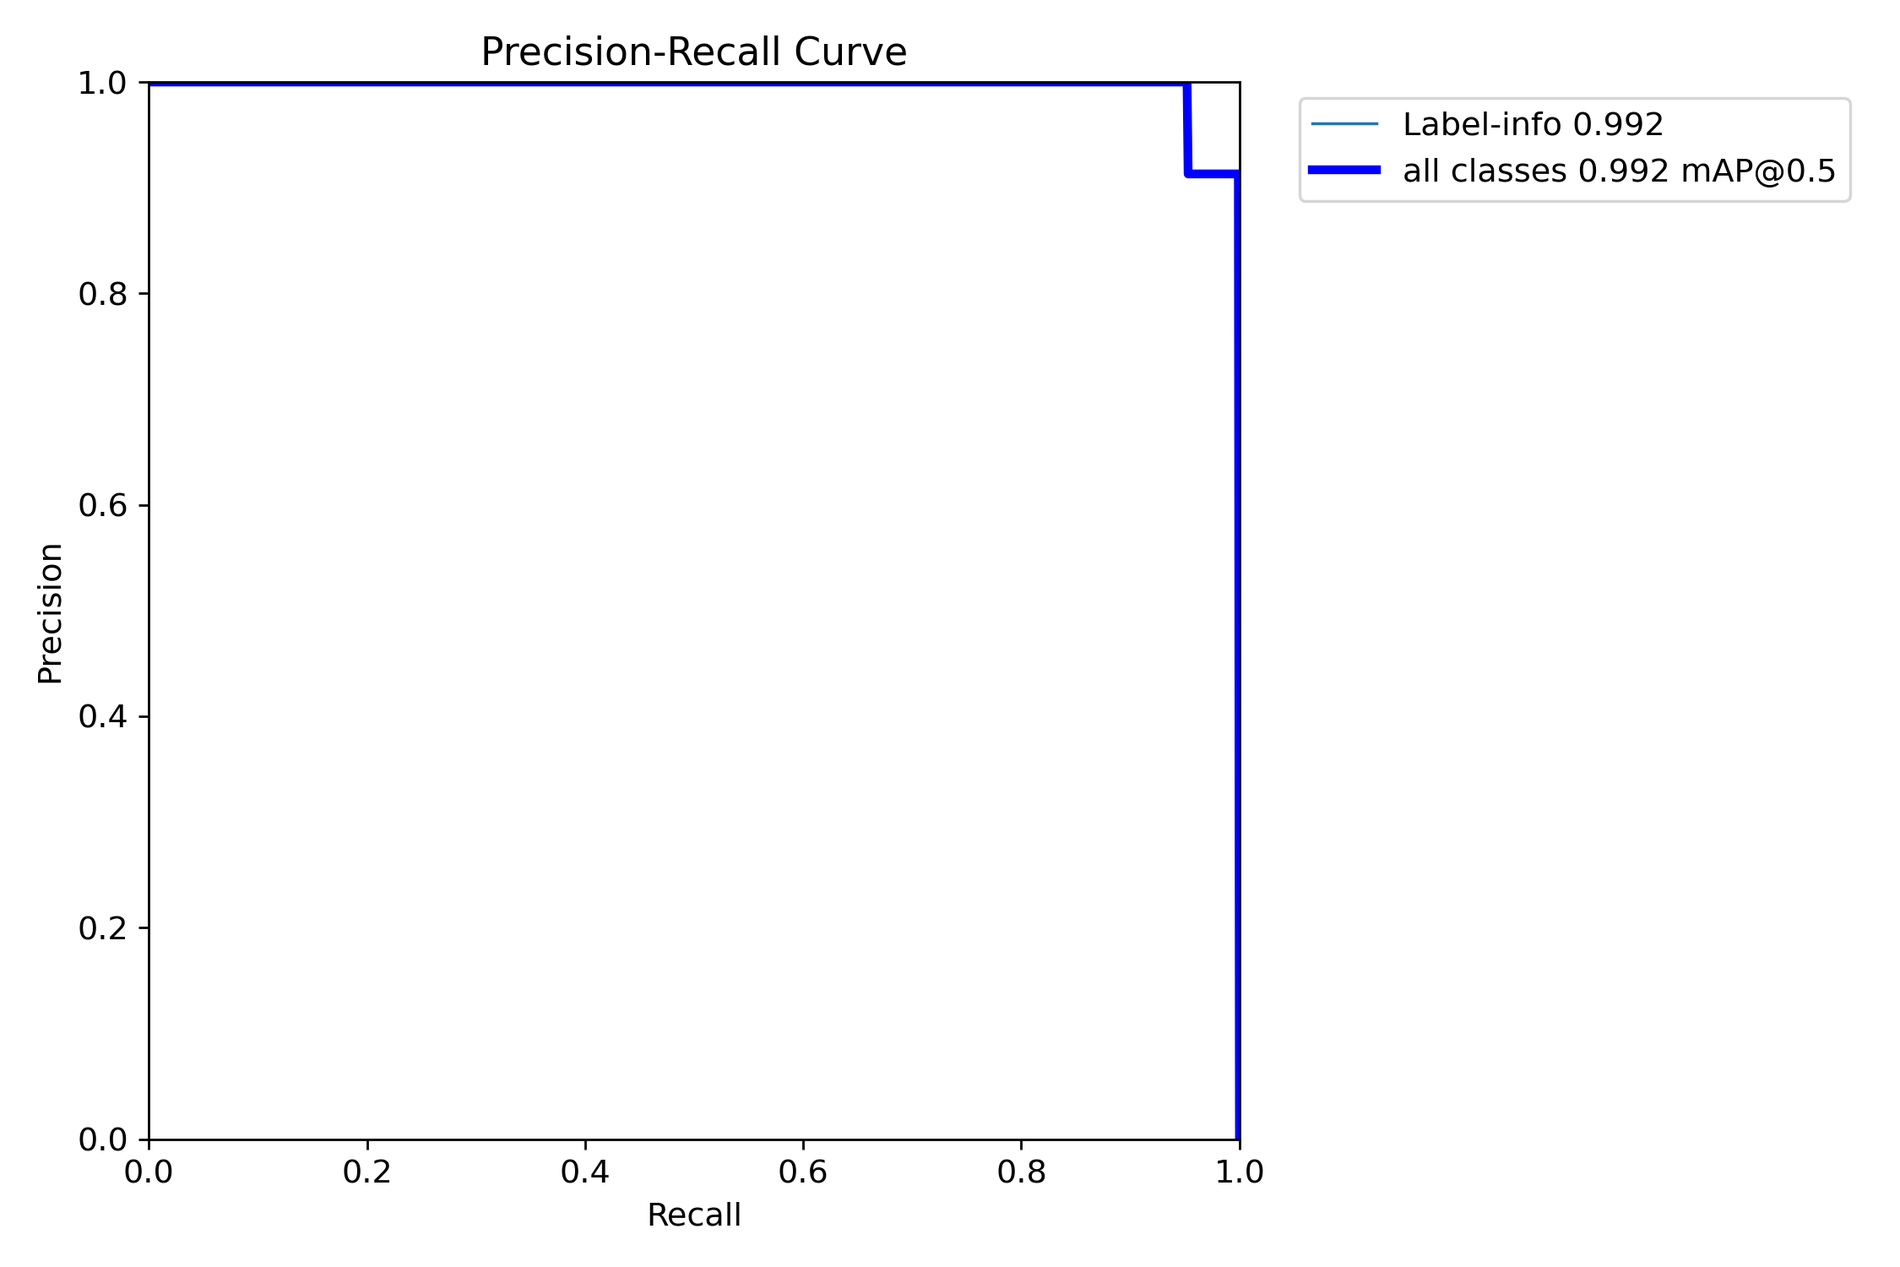
\includegraphics[width=0.78\textwidth]{Images/fig5_10.png}
\caption{Precision--recall curve of Information Region Detection.}
\label{fig:infopr}
\end{figure}

As shown in Figure~\ref{fig:infof1}, the F1 score peaks at about 0.97 at a confidence of about 0.789. The loss functions on both the training and validation sets generally trend downward, indicating that the model converges reasonably well and shows no clear sign of overfitting. However, the validation set contains a relatively small number of objects, which causes the precision and recall metrics to fluctuate strongly between epochs. Further evaluation on an independent and larger test set is therefore needed to confirm the generalization ability of the model.

\begin{figure}[htbp]
\centering
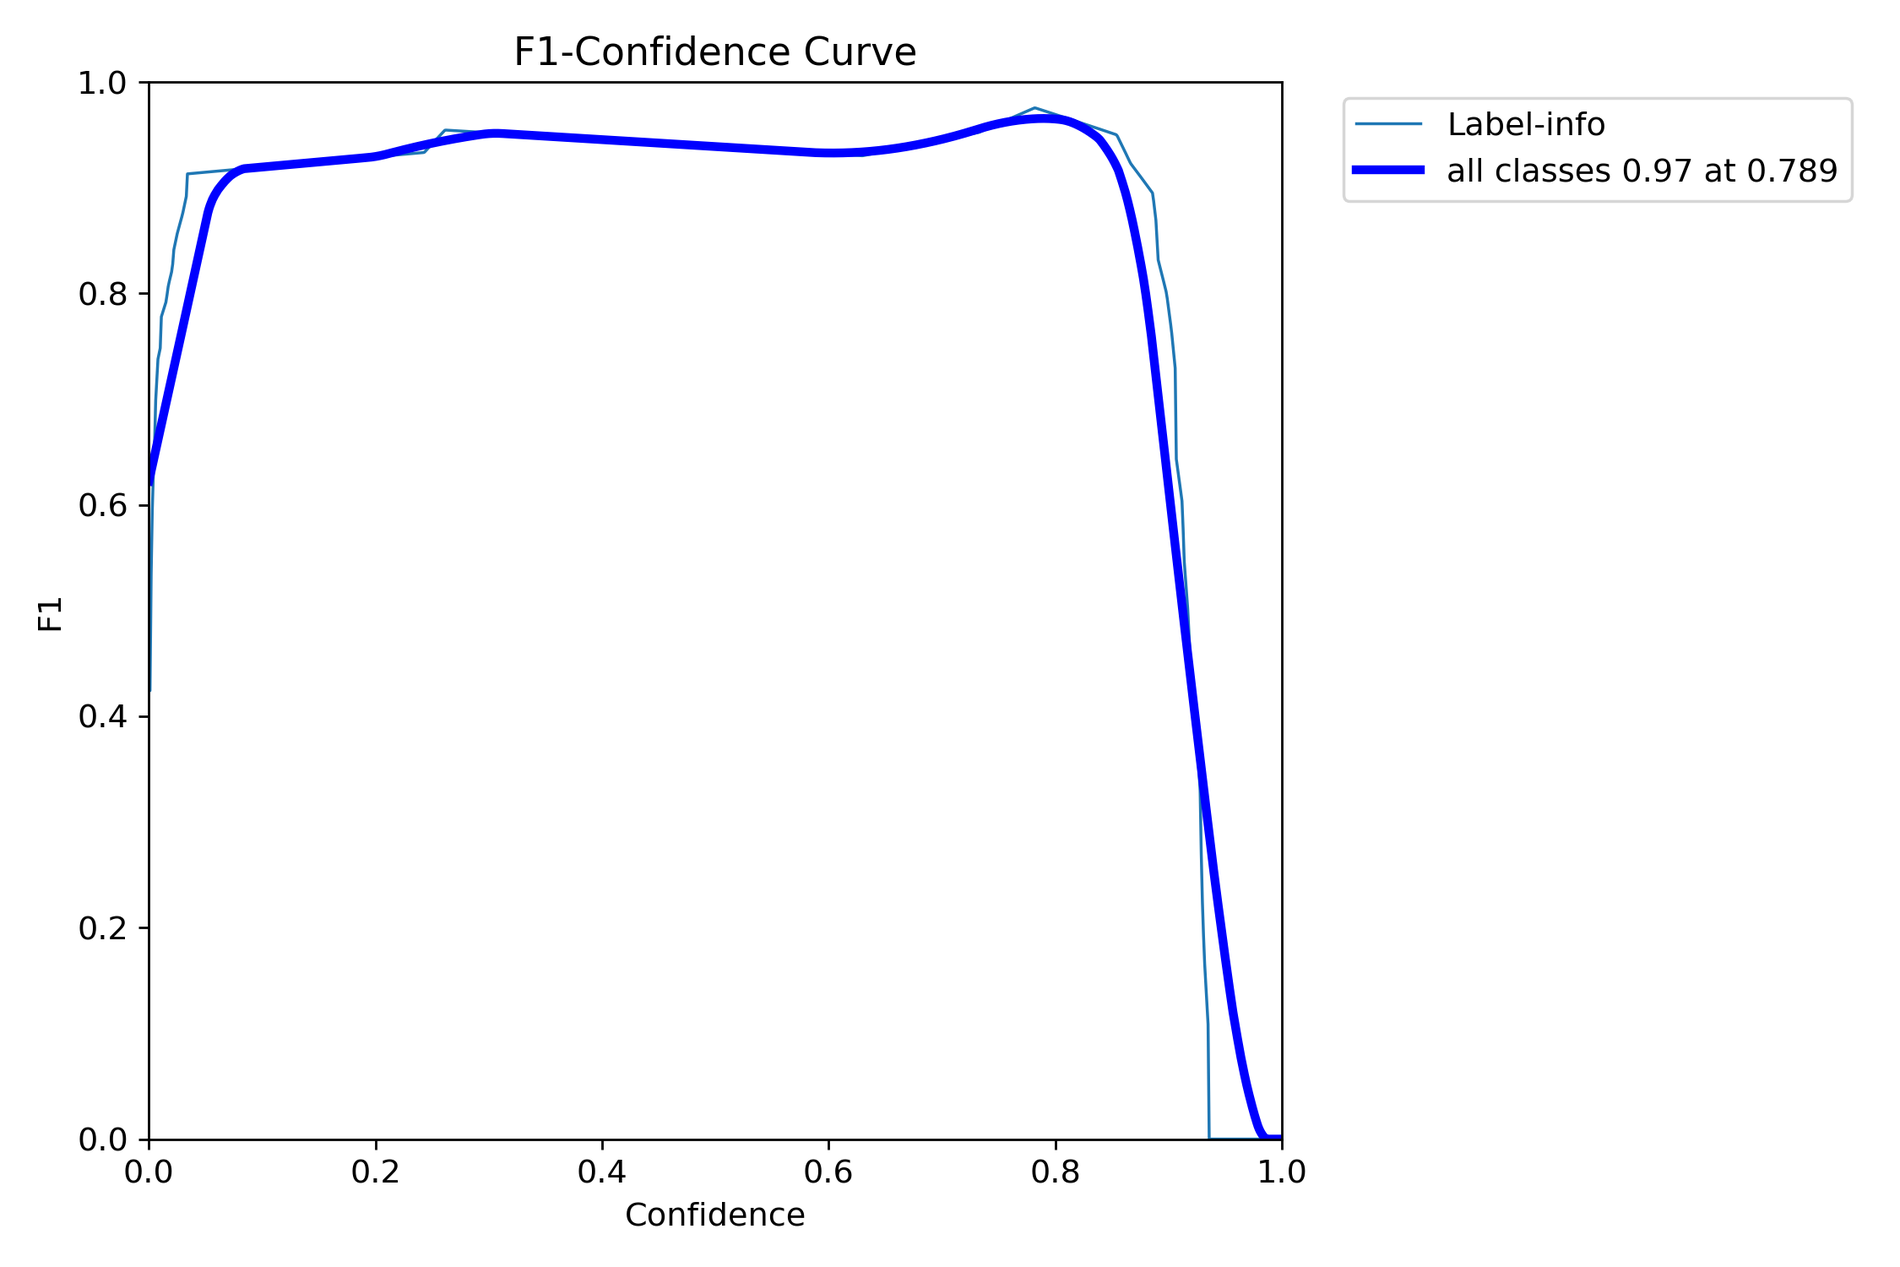
\includegraphics[width=0.78\textwidth]{Images/fig5_11.png}
\caption{F1--confidence curve of Information Region Detection.}
\label{fig:infof1}
\end{figure}

\subsection{Handwriting Recognition}

The results before and after fine-tuning TrOCR are given in Table~\ref{tab:trocrres}. After fine-tuning, the character error rate dropped to 5.39\% and the word error rate to 14.99\%. At the same time, \texttt{eval\_loss} decreased from 1.107 at step 1,000 to 0.335 at step 9,000. The checkpoint at step 9,000 was selected as the final model and saved under the name \texttt{trocr-vietnamese-final}.

\begin{table}[htbp]
\centering
\caption{TrOCR evaluation results}
\label{tab:trocrres}
\small
\begin{tabular}{R{9.0cm}cc}
\hline
\textbf{Stage} & \textbf{CER} & \textbf{WER} \\
\hline
Before fine-tuning, original \texttt{microsoft/trocr-base-handwritten} checkpoint, measured on 1,000 validation samples & 0.7250 & 1.0695 \\
After fine-tuning, \texttt{checkpoint-9000}, measured on 1,000 test samples & 0.0539 & 0.1499 \\
\hline
\end{tabular}
\end{table}

\subsection{Webcam-Based Dimension Measurement}

The results of the models supporting dimension measurement are given in Table~\ref{tab:webcammodelres}. Person Detection uses the pretrained YOLO26n model to identify and remove the person region from the image, and reaches an mAP@50--95 of 40.9\%. Hand Detection uses the YOLO26n-hand model fine-tuned on hand data and reaches an mAP@50 of 99.5\% and an mAP@50--95 of 89.8\%, showing that the model detects hands well within the scope of the test data. Parcel Detection uses a fine-tuned YOLO model to locate the parcel and create the region of interest, reaching an mAP@50 of 94.8\% and an mAP@50--95 of 85.3\%.

\begin{table}[htbp]
\centering
\caption{Results of the models in the webcam measurement pipeline}
\label{tab:webcammodelres}
\small
\begin{tabular}{llll}
\hline
\textbf{Component} & \textbf{Model} & \textbf{Metric} & \textbf{Result} \\
\hline
Person Detection & YOLO26n, pretrained & mAP@50--95 & 40.9\% \\
Hand Detection & YOLO26n-hand, fine-tuned & mAP@50 / mAP@50--95 & 99.5\% / 89.8\% \\
Parcel Detection & YOLO Package Detection & mAP@50 / mAP@50--95 & 94.8\% / 85.3\% \\
\hline
\end{tabular}
\end{table}

Besides the object detection results, the system was also evaluated through the error in dimension and volume measurement. The first experiment used a reference parcel with a horizontal width of 30.00\,cm, a depth of 22.00\,cm and a height of 10.00\,cm, corresponding to a volume of 6,600.00\,cm\textsuperscript{3}. The measurement results are given in Table~\ref{tab:webcamdim}.

\begin{table}[htbp]
\centering
\caption{Dimension and volume measurement results with webcams}
\label{tab:webcamdim}
\footnotesize
\setlength{\tabcolsep}{4pt}
\begin{tabular}{lllrrrrr}
\hline
\textbf{Trial} & \textbf{Height} & \textbf{Block} & \textbf{Length} & \textbf{Width} & \textbf{Height} & \textbf{Volume} & \textbf{Error} \\
 & \textbf{factor} & \textbf{ratio} & \textbf{(cm)} & \textbf{(cm)} & \textbf{(cm)} & \textbf{(cm\textsuperscript{3})} & \textbf{(\%)} \\
\hline
Reference & --- & --- & 30.00 & 22.00 & 10.00 & 6600.00 & 0.00 \\
1 & $0.55h$ & 32/603 & 30.25 & 22.55 & 10.24 & 6985.09 & 5.83 \\
2 & $0.56h$ & 32/603 & 30.30 & 22.55 & 10.24 & 6996.63 & 6.01 \\
3 & $0.57h$ & 32/603 & 30.30 & 22.55 & 10.35 & 7071.79 & 7.15 \\
4 & $0.55h$ & 32/605 & 30.15 & 22.48 & 10.21 & 6920.05 & 4.85 \\
5 & $0.55h$ & 32/607 & 30.05 & 22.41 & 10.17 & 6848.69 & 3.77 \\
6 & $0.55h$ & 32/608 & 30.00 & 22.37 & 10.16 & 6818.38 & 3.31 \\
7 & $0.55h$ & 32/609 & 29.95 & 22.33 & 10.14 & 6781.46 & 2.75 \\
8 & $0.55h$ & 32/614 & 29.71 & 22.15 & 10.06 & 6620.25 & 0.31 \\
\hline
Reference & --- & --- & 46.00 & 26.00 & 21.50 & 25714.00 & 0.00 \\
1 & $0.55h$ & 32/614 & 45.56 & 25.90 & 21.75 & 25665.00 & 0.19 \\
\hline
Reference & --- & --- & 47.50 & 40.00 & 28.00 & 53200.00 & 0.00 \\
1 & $0.55h$ & 32/614 & 47.50 & 39.30 & 28.79 & 53743.00 & 1.02 \\
\hline
\end{tabular}
\end{table}

As defined in Equation~\eqref{eq:pixel2cm}, the block ratio $K$ represents the actual reference length divided by its corresponding pixel length and is expressed in cm/pixel.

The experiments show that the configuration with a height correction factor of $0.55h$ and a ratio of 32/614 produces the lowest volume error, 0.31\%, for the first sample. For the other two parcels, the volume errors are 0.19\% and 1.02\% respectively. The experiments also show that the choice of the coefficient $K$ has a direct influence on the measurement result: in some cases the error on an individual edge can be large while the volume error is nonetheless lower than the result obtained with other coefficients.

\subsection{Ultrasonic-Sensor Measurement}

The overall evaluation results of the three sensors are given in Table~\ref{tab:usraw}. US1 achieves the best overall performance, with a mean absolute error of about 0.90\,cm and a mean absolute percentage error of 2.14\%. The mean absolute errors of US2 and US3 are 1.72\,cm and 1.74\,cm respectively. The results indicate that the HC-SRF05 operates more accurately on average than the two HC-SR04 sensors in this test configuration, although this difference may also be influenced by the mounting position, the measurement direction and the individual error of each device.

\begin{table}[htbp]
\centering
\caption{Overall error metrics of the three ultrasonic sensors}
\label{tab:usraw}
\small
\begin{tabular}{llrrr}
\hline
\textbf{Sensor} & \textbf{Sensor type} & \textbf{MAE (cm)} & \textbf{MAPE (\%)} & \textbf{Measurements} \\
\hline
US1 & HC-SRF05 & 0.9016 & 2.1361 & 9,700 \\
US2 & HC-SR04 & 1.7193 & 4.1628 & 9,700 \\
US3 & HC-SR04 & 1.7445 & 4.0969 & 9,700 \\
\hline
\end{tabular}
\end{table}

In the experimental setup shown in Figure~\ref{fig:ultrasonicwiring}, each sensor is placed 105\,cm from the outermost reference plane. When the parcel is placed in the measurement area, the dimension along each axis is determined by subtracting the distance from the sensor to the parcel surface from 105\,cm. Measurements at 7\,cm and from 10 to 100\,cm were used to collect sensor error data within the expected operating range of the system. The reference distances of 120, 150, 180, 200 and 220\,cm were used as an additional assessment of measurement capability beyond the main range of the setup. The results for each measurement range are given in Table~\ref{tab:usrange}.

\begin{table}[htbp]
\centering
\caption{MAE and MAPE grouped by measurement range under ideal conditions}
\label{tab:usrange}
\footnotesize
\setlength{\tabcolsep}{4pt}
\begin{tabular}{lrrrrrrr}
\hline
\textbf{Range} & \textbf{MAE} & \textbf{MAPE} & \textbf{MAE} & \textbf{MAPE} & \textbf{MAE} & \textbf{MAPE} & \textbf{Measure-} \\
\textbf{(cm)} & \textbf{US1} & \textbf{US1} & \textbf{US2} & \textbf{US2} & \textbf{US3} & \textbf{US3} & \textbf{ments} \\
\hline
7 & 0.5770 & 8.2429\% & 2.4000 & 34.2857\% & 1.4000 & 20.0000\% & 100 \\
10--19 & 0.6533 & 4.7628\% & 1.1678 & 8.0739\% & 1.1128 & 7.7297\% & 1,000 \\
20--29 & 0.8430 & 3.4635\% & 1.4223 & 5.9217\% & 1.6115 & 6.7063\% & 1,000 \\
30--39 & 0.8470 & 2.4679\% & 1.7988 & 5.2304\% & 1.8710 & 5.4779\% & 1,000 \\
40--49 & 0.8685 & 1.9614\% & 1.9212 & 4.3358\% & 1.9791 & 4.4692\% & 1,000 \\
50--59 & 1.0619 & 1.9527\% & 1.8431 & 3.3917\% & 1.7049 & 3.1488\% & 1,000 \\
60--69 & 0.9642 & 1.5070\% & 1.6324 & 2.5611\% & 1.7329 & 2.7115\% & 1,000 \\
70--79 & 0.8721 & 1.1735\% & 1.8611 & 2.5031\% & 1.8572 & 2.4988\% & 1,000 \\
80--89 & 0.8813 & 1.0454\% & 1.9419 & 2.3024\% & 1.9891 & 2.3583\% & 1,000 \\
90--99 & 1.0619 & 1.1243\% & 1.8431 & 1.9522\% & 1.7049 & 1.8096\% & 1,000 \\
100 & 1.2970 & 1.2970\% & 1.8450 & 1.8450\% & 2.3430 & 2.3430\% & 100 \\
120 & 0.9990 & 0.8325\% & 1.5940 & 1.3283\% & 2.0430 & 1.7025\% & 100 \\
150 & 1.1570 & 0.7713\% & 1.7010 & 1.1340\% & 2.0480 & 1.3653\% & 100 \\
180 & 1.1630 & 0.6461\% & 1.8120 & 1.0067\% & 2.0540 & 1.1411\% & 100 \\
200 & 0.8370 & 0.4185\% & 1.2490 & 0.6245\% & 1.5860 & 0.7930\% & 100 \\
220 & 0.8950 & 0.4068\% & 1.8550 & 0.8432\% & 2.1120 & 0.9600\% & 100 \\
\hline
\end{tabular}
\end{table}

Each tested reference distance was measured 100 times. To keep Table~\ref{tab:usrange} concise, the results from 10 to 99\,cm were aggregated into 10\,cm ranges, while the results at 7, 100, 120, 150, 180, 200 and 220\,cm were retained as individual rows. US1 has the lowest grouped MAE across all measurement ranges. The mean absolute percentage error of all three sensors generally decreases as the distance increases, because the same absolute error accounts for a smaller proportion at larger distances. A lower percentage error at long range therefore does not mean that the absolute error always decreases.

These results were collected under ideal conditions, with the sensor pointing directly at a flat surface and no obstacle near the emission area. In the actual configuration, a wooden bar or a wall close to the sensor can reflect the ultrasonic wave, causing the sensor to pick up the wrong signal and return an inaccurate distance. For this reason, the sensor heads are positioned to protrude at least 15\,cm beyond the nearest wall or support bar in order to limit this effect.

\subsection{Shipping Fee Calculation}

The test cases of the fee calculation module are given in Table~\ref{tab:feetest}. The expected values were computed manually from the weight tiers and unit prices in the 2026 tariff table \cite{vnpost_tariff2026} (see Appendix~B).

\begin{table}[htbp]
\centering
\caption{Test results of the fee calculation module}
\label{tab:feetest}
\small
\begin{tabular}{R{3.0cm}R{3.8cm}R{5.6cm}}
\hline
\textbf{Test case} & \textbf{Main input} & \textbf{Expected result} \\
\hline
Weight below the volumetric threshold & 2\,kg, $L=30$, $W=20$, $H=15$, all at most 50\,cm & \texttt{weight\_chargeable} $=2$\,kg, \texttt{used\_volumetric} $=$ false \\
Weight above the volumetric threshold & 1\,kg, $L=60$, $W=50$, $H=40$ & \texttt{weight\_volumetric} $=20$\,kg, so \texttt{weight\_chargeable} $=20$\,kg, \texttt{used\_volumetric} $=$ true \\
ETN011 price within the base tier & 750\,g, intra-province route & Correctly looks up the 1000\,g tier and takes the corresponding base price \\
ETN011 price above the threshold & 3000\,g, intra-province route, base 21,000 VND, \texttt{base\_limit} 2000\,g & Extra 1000\,g gives 2 units at 1,600 VND, that is 3,200 VND; total 24,200 VND \\
CTN001 progressive price & 5000\,g, intra-province route, base 30,507.84 VND, \texttt{base\_limit} 2000\,g & 3 units of 1000\,g at 4,134.24 VND, that is 12,402.72 VND; total 42,910.56 VND \\
\hline
\end{tabular}
\end{table}

All five test cases match the values computed by hand from the formulas in the algorithm design document, showing that the pipeline behaves correctly on the main logical branches, namely province normalization, route determination, volumetric weight, tiered price and progressive price. Further test cases should be added for edge cases such as invalid or completely incorrect province names, weights exactly at the boundary between two price tiers, and the special routes involving Đà Nẵng, Hà Nội and TP.HCM in the ETN service, in order to ensure full test coverage.

\section{Qualitative Results}

\subsection{Box/Envelope Detection}

Figure~\ref{fig:qualbox} shows representative detection results. YOLO11n detects and distinguishes the two object groups, envelope and box, with relatively high confidence. Most objects are detected correctly, with confidence scores in the range of about 0.9 to 1.0, and the bounding boxes tend to cover the object region fully. The model maintains its recognition ability under varying conditions of camera angle, colour, size and surrounding environment. However, some cases with unusual shapes or object orientations can still reduce the accuracy of the detected region. Overall, the model performs its object recognition role well in the first stage of the system.

\begin{figure}[htbp]
\centering
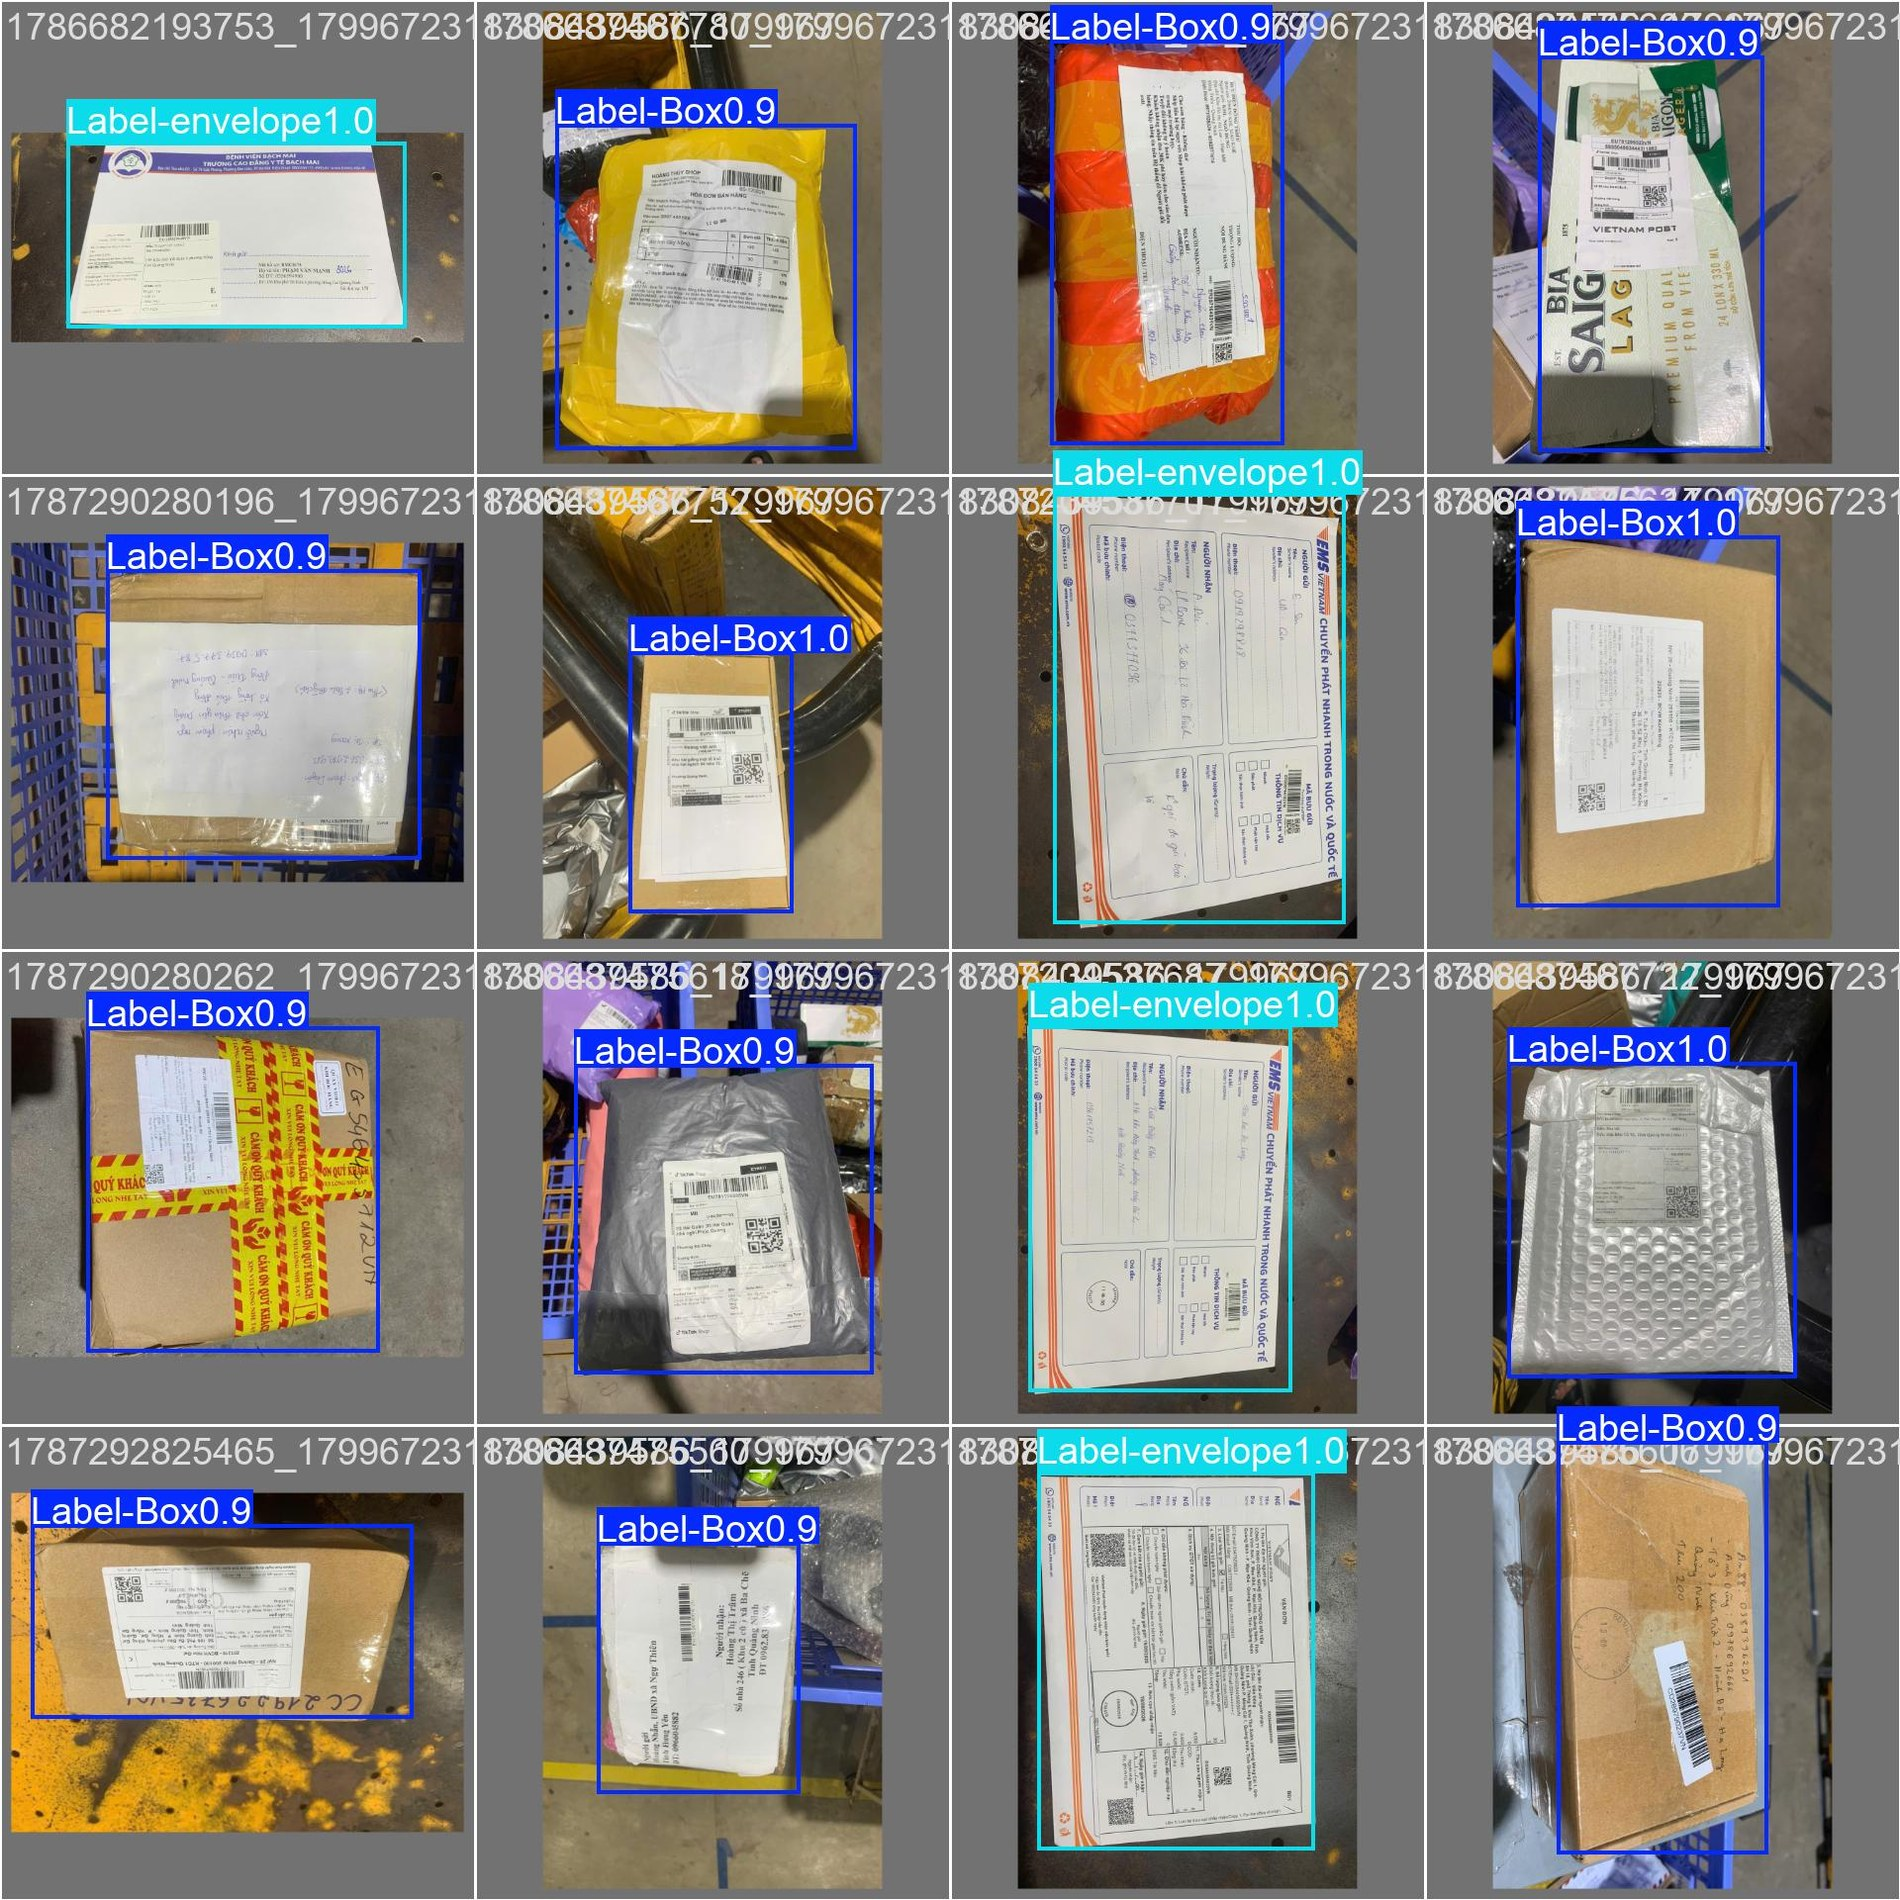
\includegraphics[width=\textwidth]{Images/fig5_12.jpg}
\caption{Parcel and envelope detection results.}
\label{fig:qualbox}
\end{figure}

\subsection{Information Region Detection}

Figure~\ref{fig:qualinfo} shows representative results of the information region detector. The model detects information regions relatively well, with confidence scores mainly in the range 0.8 to 0.9. The bounding boxes generally cover the label and shipping form area accurately across many parcel types and camera angles. This result shows that the model is suitable for identifying the input information region for the subsequent OCR step.

\begin{figure}[htbp]
\centering
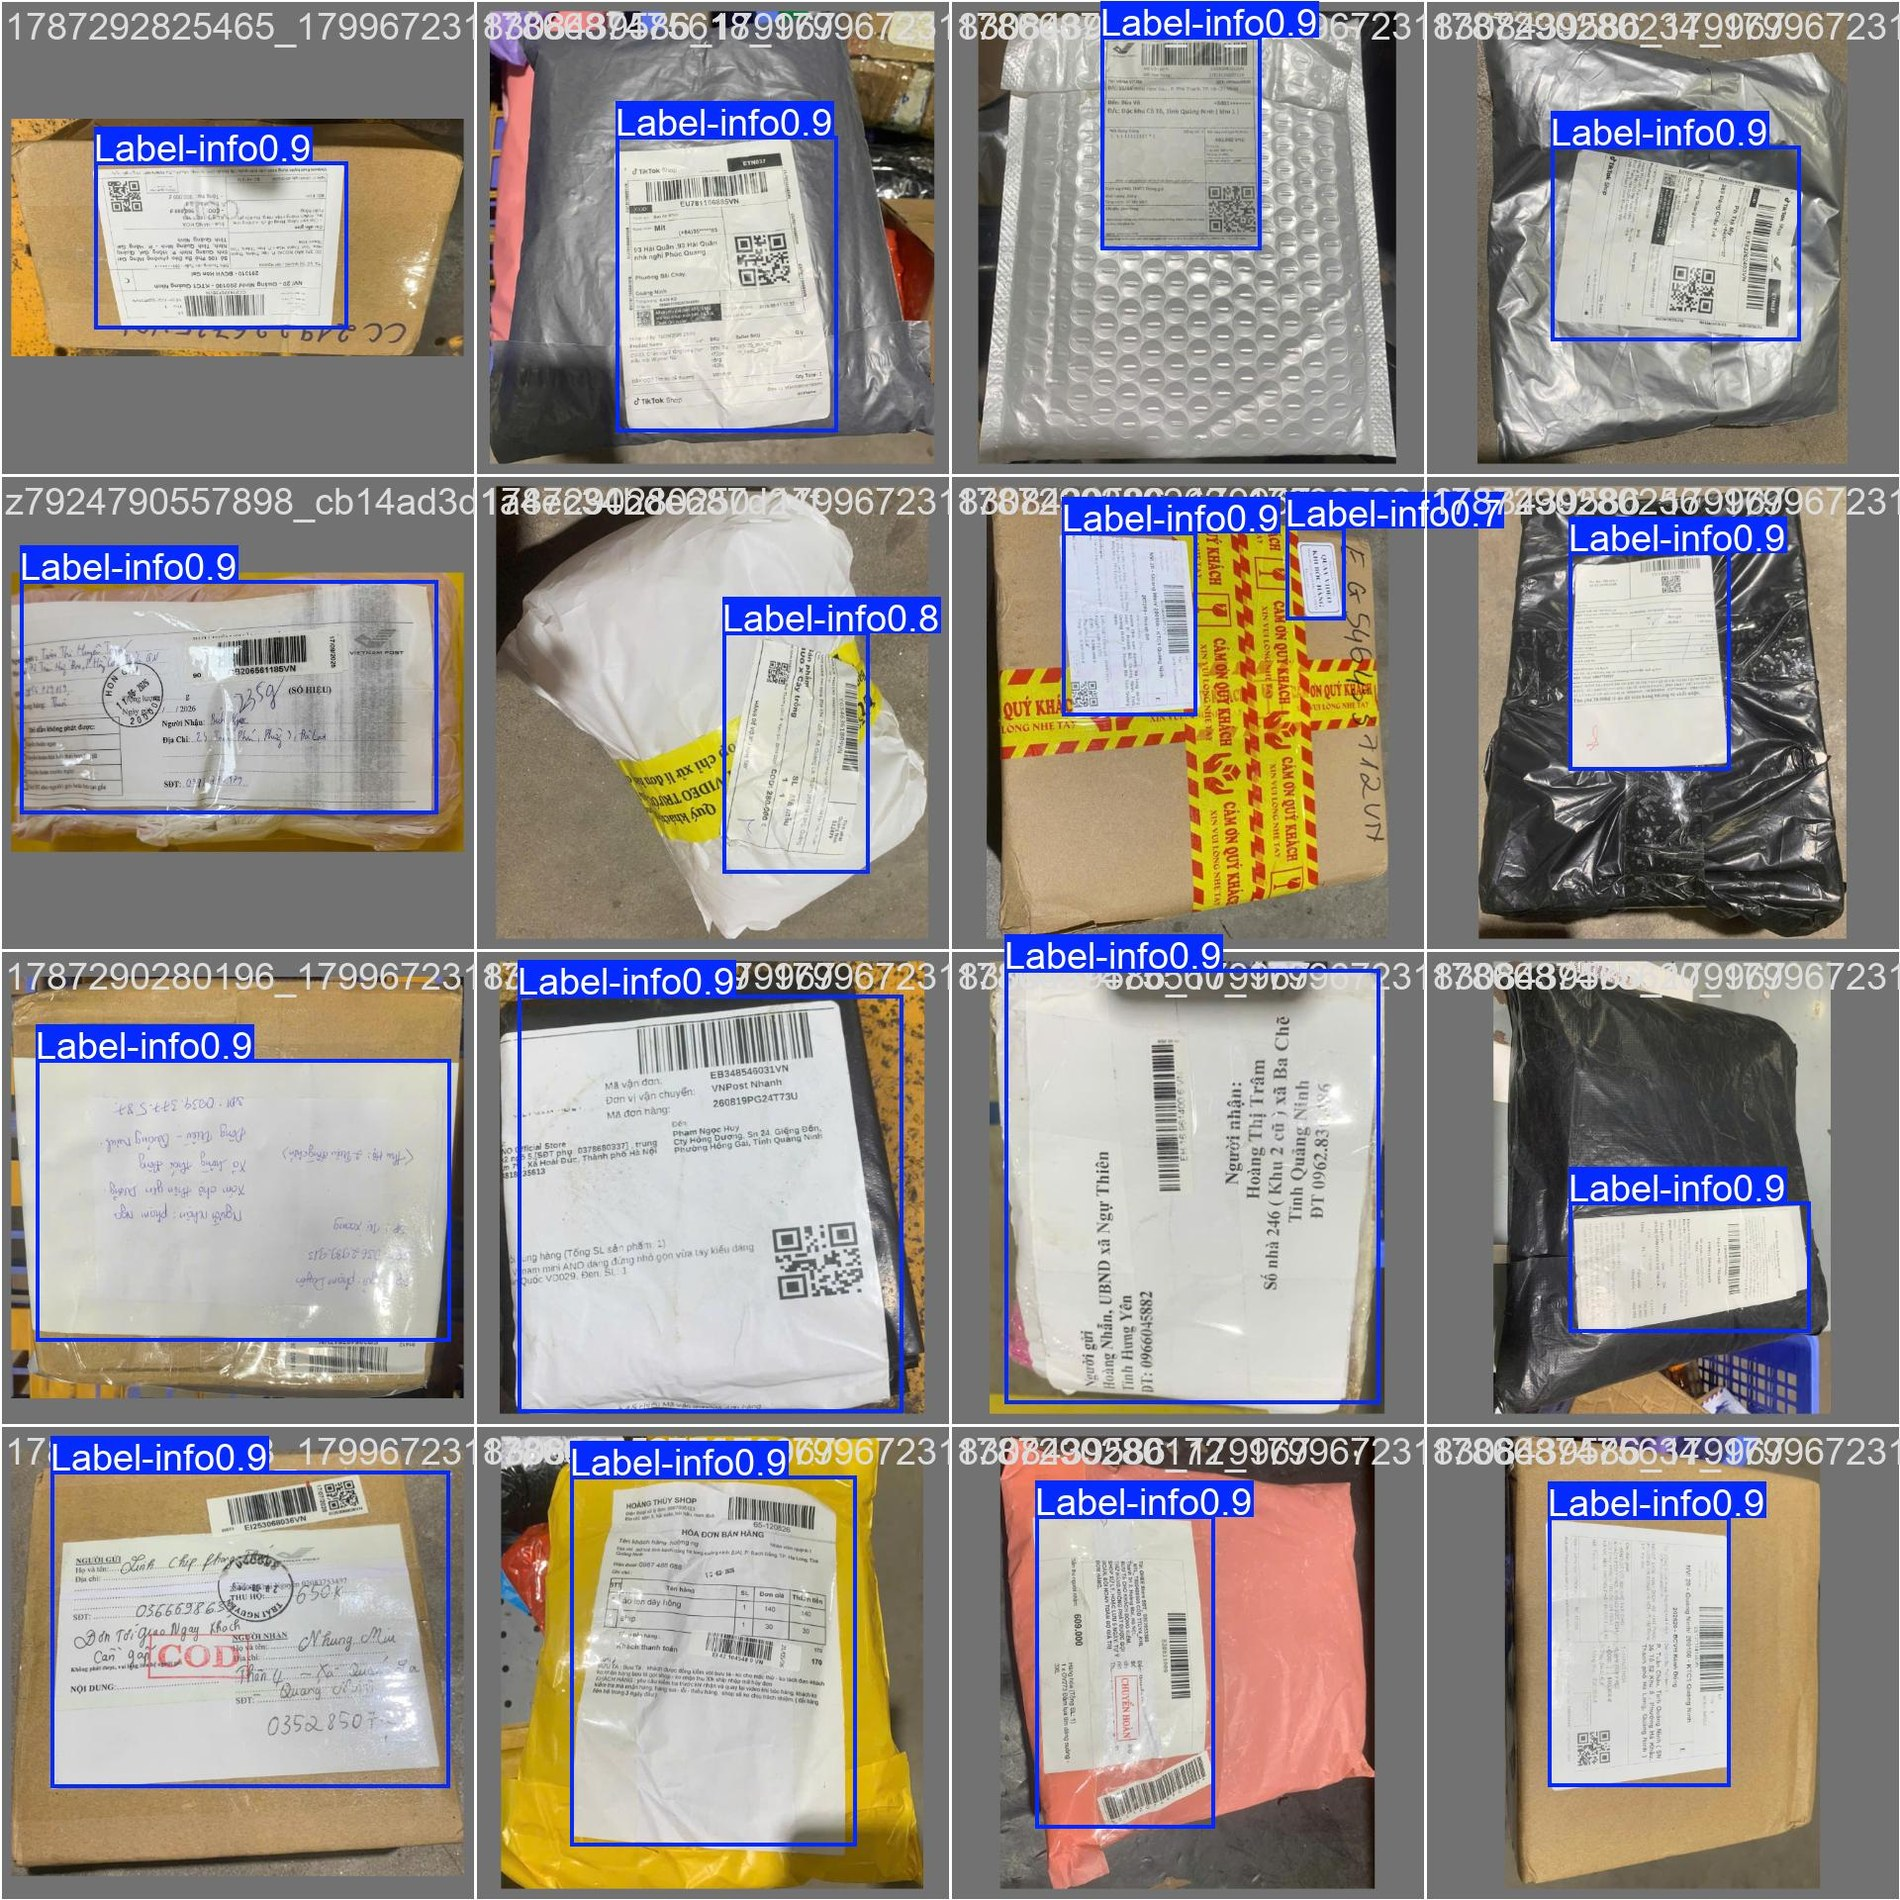
\includegraphics[width=\textwidth]{Images/fig5_13.jpg}
\caption{Information region detection results on parcels.}
\label{fig:qualinfo}
\end{figure}

\subsection{Webcam-Based Dimension Measurement}

Figure~\ref{fig:qualhand} shows the hand and parcel detection results. The keypoints identify the hand region, while the bounding box of the parcel is used to create the region of interest.

\begin{figure}[htbp]
\centering
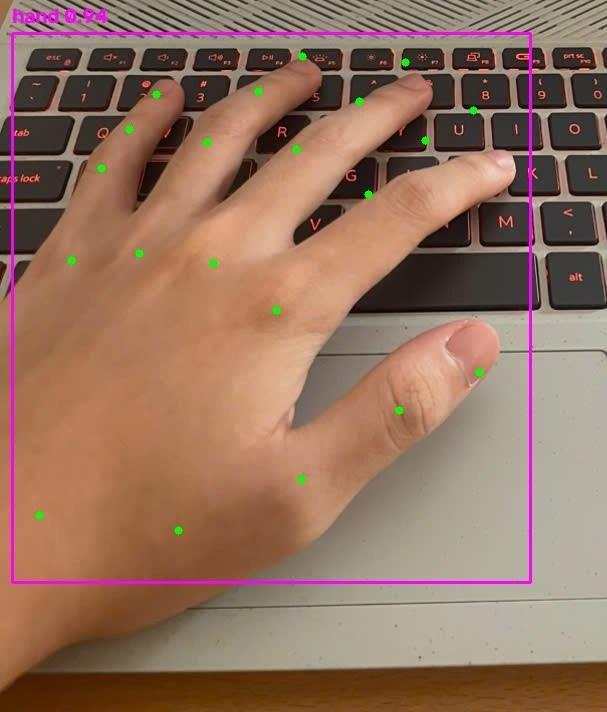
\includegraphics[width=0.48\textwidth]{Images/fig5_14a.jpg}\hfill
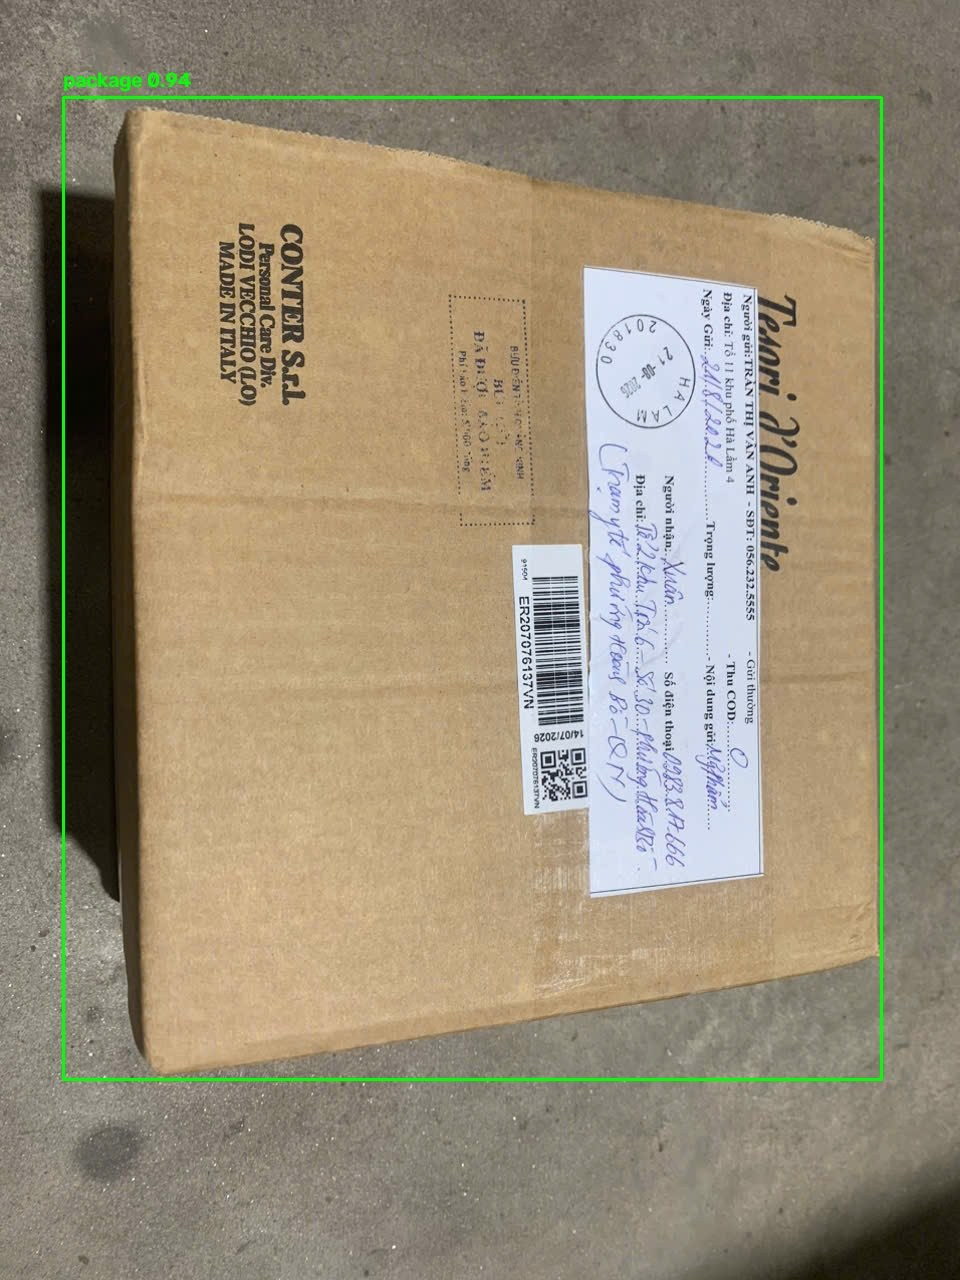
\includegraphics[width=0.48\textwidth]{Images/fig5_14b.jpg}
\caption{Hand and parcel detection results.}
\label{fig:qualhand}
\end{figure}

Figure~\ref{fig:qualperson} shows the person detection result. The person region is identified so that it can be excluded from edge detection and parcel dimension measurement.

\begin{figure}[htbp]
\centering
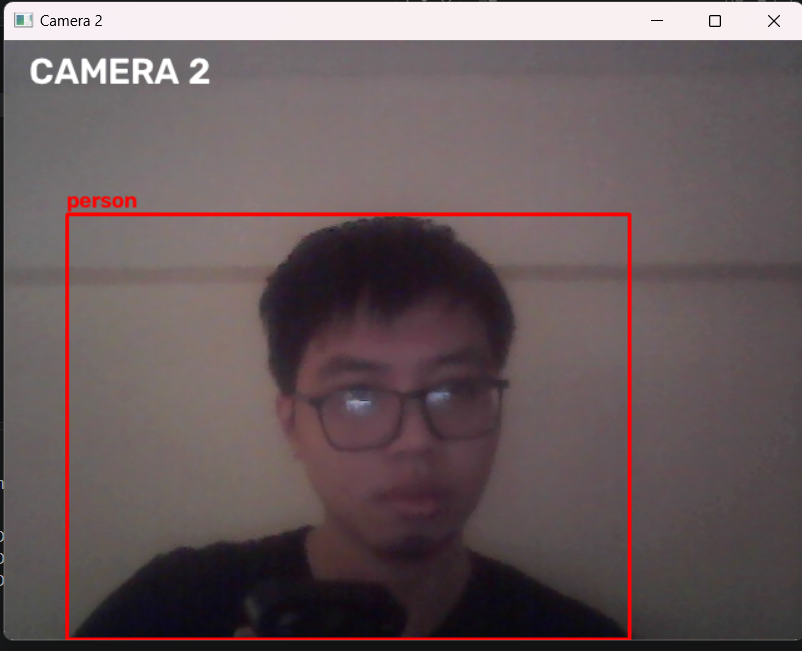
\includegraphics[width=0.78\textwidth]{Images/fig5_15.png}
\caption{Person detection results.}
\label{fig:qualperson}
\end{figure}

Figure~\ref{fig:qualnoise} illustrates a failure mode: a distracting object appearing close to the parcel can affect the determination of the region of interest and the boundary.

\begin{figure}[htbp]
\centering
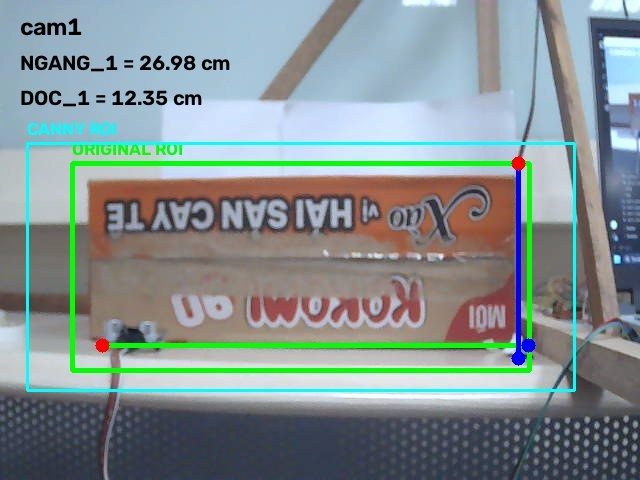
\includegraphics[width=0.78\textwidth]{Images/fig5_16.jpg}
\caption{Effect of a distracting object on edge detection results.}
\label{fig:qualnoise}
\end{figure}

Figure~\ref{fig:qualdim} shows a complete measurement. Under suitable lighting, with a contrasting background and the parcel fully within the field of view, the system identifies the edges and computes the three dimensions. After repeated experiments on different parcels, the system achieved a volume error of 0.31\% under suitable lighting and background conditions; when the lighting and background conditions are not guaranteed, the volume error can rise to about 5\%.

\begin{figure}[htbp]
\centering
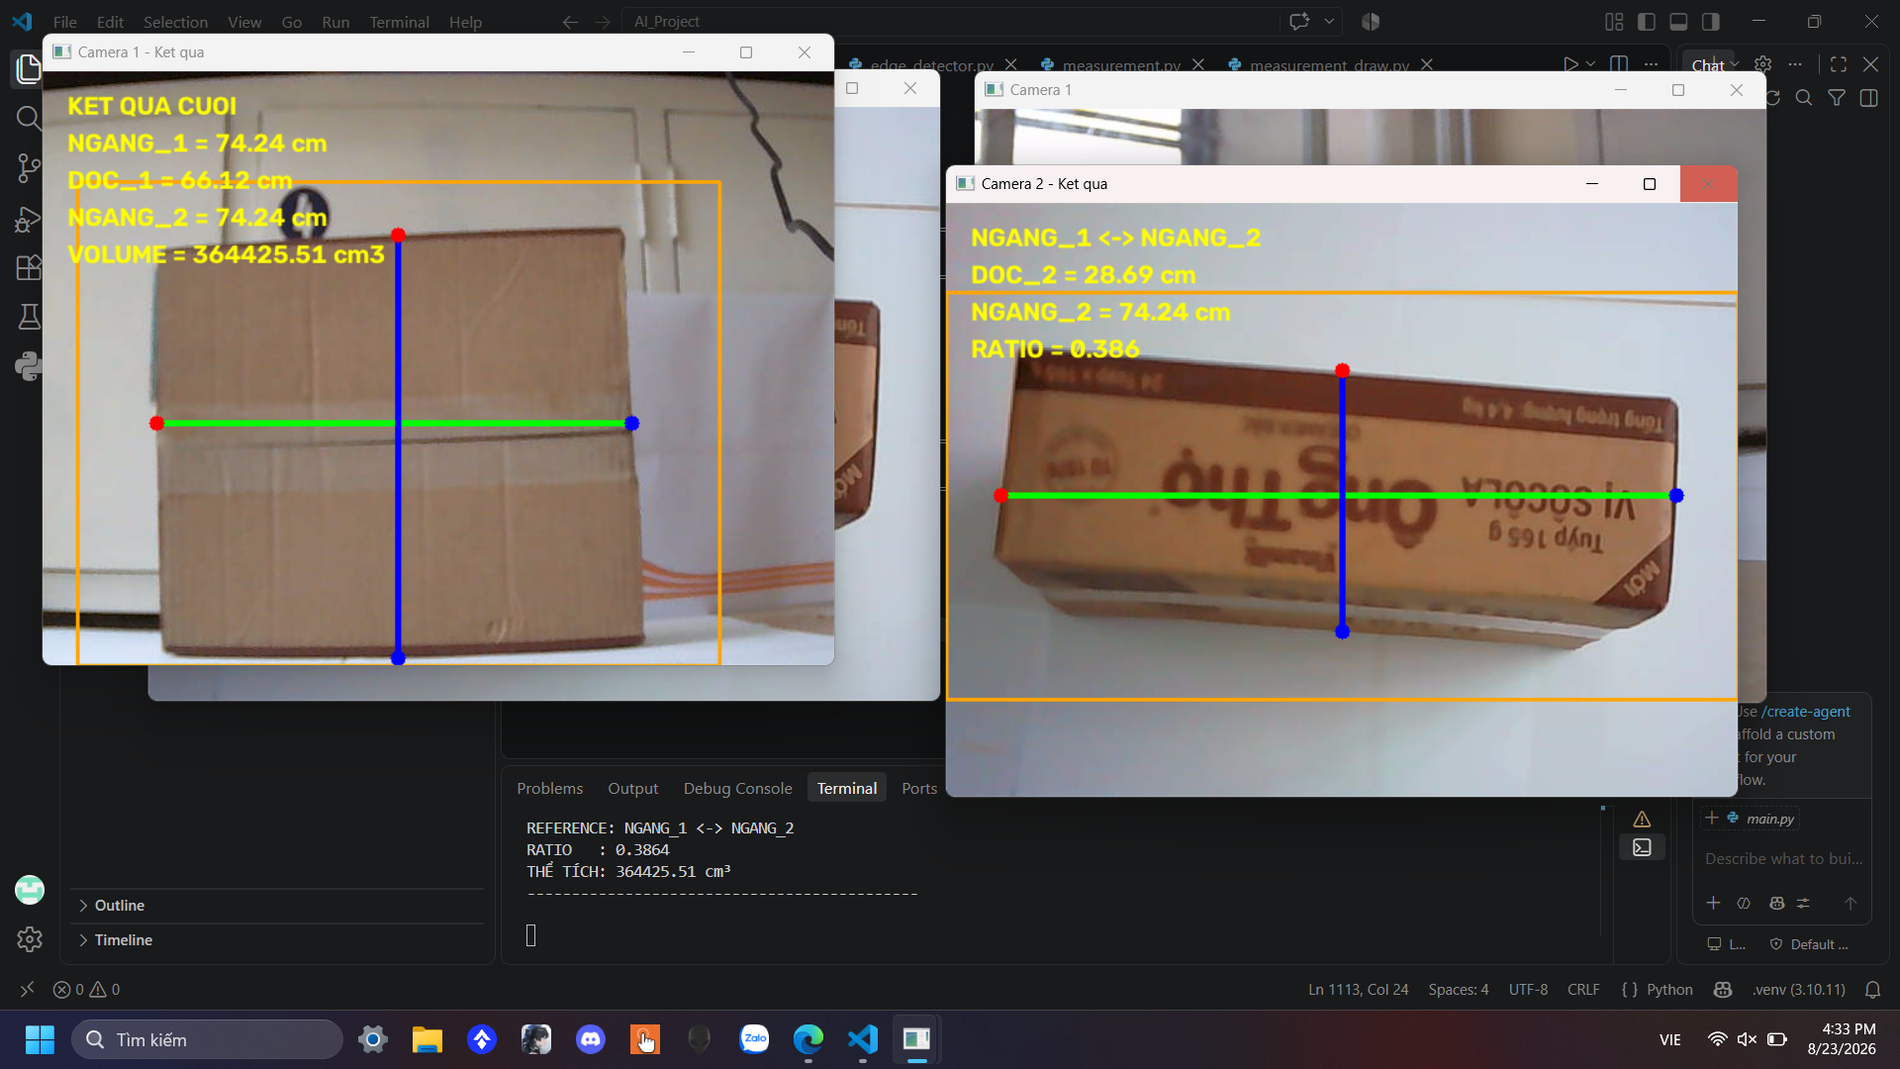
\includegraphics[width=\textwidth]{Images/fig5_17.png}
\caption{Parcel dimension measurement results using two cameras.}
\label{fig:qualdim}
\end{figure}

\section{Error Analysis and Discussion}

\textbf{Parcel and envelope classification.} Classification still struggles under conditions that differ from the training data, for example when the envelope is held in the hand, stood upright or placed near the edge of the table. Parcels with elongated shapes, deformed parcels or parcels wrapped in transparent plastic can also reduce recognition performance, especially when the image quality is low or the scene contains many distracting objects. The main cause is that the data does not fully cover the diversity of postal item orientations, shapes and contexts. In addition, the lack of background images without any postal item means that the system does not reliably identify the case where no object is present in the frame. To improve this, the dataset needs additional images taken in a wider range of orientations and environmental conditions, parcels with unusual shapes, and negative background images.

\textbf{Information region detection.} The detector sometimes produces false detections when patterns, printed text on the box or high-contrast areas resemble an information label. The evaluation results may also not fully reflect generalization ability, since the validation set contains only 22 images. It is therefore necessary to add parcel samples with more diverse surfaces and labels, and to evaluate on a larger independent test set.

\textbf{Handwriting recognition.} Errors still occur when the strokes are unclear or when characters have similar shapes. Recorded cases include ``dừng lại'' being recognized as ``đừng lại'' and ``tường trình'' as ``tường linh vị''. The system may also alter symbol representations, for example turning \texttt{->} into an arrow, converting \texttt{VSV} into \texttt{vsv}, or adding and omitting punctuation. The cause may lie in the difference between the training data and real photographs, particularly in slant, blur, lighting and special symbols. This could be improved by adding data closer to real shipping forms and applying augmentation to simulate the capture conditions at a kiosk.

\textbf{Webcam-based dimension measurement.} Measurement depends heavily on image quality, background contrast and the degree of parcel occlusion. Distracting objects and backgrounds with a colour similar to the parcel can also produce inaccurate boundaries, as illustrated in Figure~\ref{fig:qualnoise}. Furthermore, the volume is computed as the product of three dimensions, so errors on the individual edges can accumulate in the final result.

\textbf{Ultrasonic measurement.} Measurement is still affected by the individual deviation of each sensor and by the surfaces around the measurement area. Because the ultrasonic wave is emitted as a beam, walls, wooden bars or objects near the propagation path can create unwanted reflections, causing the sensor to pick up the wrong echo signal and return a distance shorter than the real one. In the current setup, the sensor heads are positioned to protrude at least 15\,cm beyond the surrounding surfaces in order to limit this effect. Even so, data still needs to be collected directly on the actual measurement frame in order to assess the error and build a suitable correction factor for each sensor.

\chapter{Conclusion}
\label{chap:conclusion}

\section{Summary of Achievements}

Postal item acceptance at the counter currently depends on many manual operations, such as entering customer information, weighing, measuring dimensions and calculating the fee. This makes a transaction take about 6--8 minutes and can lead to data-entry errors. The project therefore built a system that combines artificial intelligence with low-cost sensors in order to automate part of this workflow.

The system supports item classification, information extraction, dimension measurement, volume estimation and fee calculation. YOLO11n is used to classify parcels and envelopes and to detect the information region on parcels. EasyOCR detects the text regions and a fine-tuned TrOCR recognizes Vietnamese handwriting. Parcel dimensions are determined by one of two methods: webcams combined with YOLO and Canny edge detection, or three ultrasonic sensors connected to an ESP32 together with a temperature sensor.

The results show that the item classification model and the information region detection model reach an mAP@50 of 99.50\% and 97.90\% respectively. TrOCR achieves a character error rate of 5.39\% and a word error rate of 14.99\%. With the webcam method, the volume errors on the three test samples are 0.31\%, 0.19\% and 1.02\%. With the ultrasonic method, the mean absolute error of the three sensors lies between 0.9016 and 1.7445\,cm. The fee calculation module also matches manual computation in every test case.

Overall, the project has built the core components of a system supporting postal item acceptance. The results show that combining AI models with low-cost equipment is feasible under test conditions. However, because the complete system has not been evaluated at a post office counter, the project does not yet have sufficient grounds to conclude that it can shorten transaction time or reduce manual data entry in practice.

\section{Limitations and Future Work}

The data available to the project is limited. The Postal Item Dataset contains only 439 images and therefore does not fully cover the range of postal item types, object orientations and environmental conditions. Viet-Handwriting-OCR-v2 was not built specifically for postal shipping forms, and training did not apply augmentation. The ability to recognize slanted handwriting, smudged ink, uneven lighting or low-quality images has therefore not been fully assessed.

The dimension measurement methods are also affected by the test conditions. The webcam method depends on lighting, background, camera placement, parcel orientation and occlusion by the hand. The volume error was evaluated on only three samples, so it is not highly representative. The ultrasonic method can be disturbed by objects or surfaces near the wave propagation area, and each sensor has a different error level and needs to be calibrated individually.

In addition, the components have mainly been tested in isolation rather than evaluated end to end. The system is not connected to an electronic scale, the operational software or the official tariff table, and it has not been tested directly at a post office counter. The stability and real-world effectiveness of the system therefore remain undetermined.

In future work, the data needs to be expanded with a wider range of postal item types, orientations, lighting conditions and occlusion cases. The OCR data should include images of real shipping forms and apply augmentation. Both measurement methods need to be evaluated on more parcels within a standardized measurement area; for the ultrasonic method in particular, calibration should continue and a mechanism for discarding anomalous measurements should be added. Finally, the components need to be integrated with an electronic scale, the operational software and the official tariff table so that the complete workflow can be tested at a post office. Those results would provide a more reliable basis for assessing whether the system can be deployed in practice.

% ---------- References ----------
% Heading of the reference list, followed by a note on the citation conventions
% used: how Vietnamese author names are written, and which entries are software
% or product documentation rather than peer-reviewed publications.
\renewcommand{\bibname}{References\\[0.8em]
  \normalfont\normalsize\mdseries
  \begin{minipage}{\textwidth}\setstretch{1.2}\noindent
  \textit{Conventions.} The list is divided into three groups by source type, so
  that peer-reviewed work is not presented as equivalent to product
  documentation. Group~A contains peer-reviewed publications and textbooks.
  Group~B contains software documentation, model cards, public datasets and
  hardware datasheets; these are cited to identify the tools and data used, not
  as scientific evidence. Group~C contains unpublished internal documents of
  Quang Ninh Provincial Post Office; they are not publicly available, and the
  business rules and tariff tables cited from them are reproduced in
  Appendices~A and~B. Numbering is continuous across the three groups. Vietnamese
  author names are given in full, in the order used by the cited source, rather
  than abbreviated to initials.
  \end{minipage}}
\clearpage\phantomsection\addcontentsline{toc}{chapter}{References}
% ---------------------------------------------------------------------
% Reference list, written out directly rather than generated by BibTeX.
%
% IEEEtran cannot produce the A/B/C group headings that separate
% peer-reviewed work from software documentation and internal documents,
% so the list is maintained here by hand. references.bib is kept in the
% project as the underlying source data but is not compiled.
%
% To add an entry: put a \bibitem{key} in the right group; cite it with
% \cite{key} as usual. Numbering follows the order below.
% ---------------------------------------------------------------------

\begin{thebibliography}{10}
\providecommand{\url}[1]{#1}
\csname url@samestyle\endcsname
\providecommand{\newblock}{\relax}
\providecommand{\bibinfo}[2]{#2}
\providecommand{\BIBentrySTDinterwordspacing}{\spaceskip=0pt\relax}
\providecommand{\BIBentryALTinterwordstretchfactor}{4}
\providecommand{\BIBentryALTinterwordspacing}{\spaceskip=\fontdimen2\font plus
\BIBentryALTinterwordstretchfactor\fontdimen3\font minus \fontdimen4\font\relax}
\providecommand{\bibgroup}[1]{\item[]\hspace{-\labelwidth}\hspace{-\labelsep}%
{\normalfont\bfseries #1}\vspace{2pt}}

\bibgroup{A. Peer-reviewed publications and textbooks}

\bibitem{li2023trocr}
M.~Li, T.~Lv, J.~Chen, L.~Cui, Y.~Lu, D.~Florencio, C.~Zhang, Z.~Li, and F.~Wei,
  ``{TrOCR}: Transformer-based optical character recognition with pre-trained
  models,'' \emph{Proceedings of the AAAI Conference on Artificial
  Intelligence}, vol.~37, no.~11, pp. 13094--13102, 2023. [Online]. Available:
  \url{https://ojs.aaai.org/index.php/AAAI/article/view/26538}

\bibitem{fernandes2006}
L.~A.~F. Fernandes, M.~M. Oliveira, R.~da~Silva, and G.~J. Crespo, ``A fast and
  accurate approach for computing the dimensions of boxes from single
  perspective images,'' \emph{Journal of the Brazilian Computer Society},
  vol.~12, no.~1, pp. 19--30, 2006. [Online]. Available:
  \url{https://journal-bcs.springeropen.com/articles/10.1007/BF03192392}

\bibitem{peng2020}
T.~Peng, Z.~Zhang, F.~Chen, and D.~Zeng, ``Dimension measurement and key point
  detection of boxes through laser-triangulation and deep learning-based
  techniques,'' \emph{Applied Sciences}, vol.~10, no.~1, Art. no.~26, 2020.
  [Online]. Available: \url{https://www.mdpi.com/2076-3417/10/1/26}

\bibitem{lethai2019}
Lê Văn Thái, ``{Ứng dụng camera 3D trong việc phân loại sản phẩm theo hình dạng
  và kích thước},'' Undergraduate thesis, Ho Chi Minh City University of
  Technology and Education, 2019. [Online]. Available:
  \url{https://www.slideshare.net/slideshow/luan-van-ung-dung-camera-3d-trong-phan-loai-san-pham-hay/206571728}

\bibitem{tran2026}
Thien Tran Van, Hiroshi Hasegawa, and Ngoc Tam Bui, ``Unified parcel attribute
  recognition: An efficient edge-based system using {YOLOv12-BiFPN-ResCBAM} for
  barcode, dimensioning, and damage detection,'' \emph{Journal of Real-Time
  Image Processing}, vol.~23, Art. no.~110, 2026. [Online]. Available:
  \url{https://link.springer.com/article/10.1007/s11554-026-01908-x}

\bibitem{redmon2016}
J.~Redmon, S.~Divvala, R.~Girshick, and A.~Farhadi, ``You only look once:
  Unified, real-time object detection,'' in \emph{Proceedings of the IEEE
  Conference on Computer Vision and Pattern Recognition}, 2016, pp. 779--788.
  [Online]. Available:
  \url{https://openaccess.thecvf.com/content_cvpr_2016/html/Redmon_You_Only_Look_CVPR_2016_paper.html}

\bibitem{baek2019craft}
Y.~Baek, B.~Lee, D.~Han, S.~Yun, and H.~Lee, ``Character region awareness for
  text detection,'' in \emph{Proceedings of the IEEE/CVF Conference on Computer
  Vision and Pattern Recognition}, 2019, pp. 9365--9374. [Online]. Available:
  \url{https://openaccess.thecvf.com/content_CVPR_2019/html/Baek_Character_Region_Awareness_for_Text_Detection_CVPR_2019_paper.html}

\bibitem{canny1986}
J.~Canny, ``A computational approach to edge detection,'' \emph{IEEE
  Transactions on Pattern Analysis and Machine Intelligence}, vol. PAMI-8,
  no.~6, pp. 679--698, 1986. [Online]. Available:
  \url{https://ieeexplore.ieee.org/document/4767851}

\bibitem{openstax_sound}
OpenStax, ``17.2 speed of sound,'' in \emph{University Physics Volume 1}. Rice
  University. [Online]. Available:
  \url{https://openstax.org/books/university-physics-volume-1/pages/17-2-speed-of-sound}

\bibgroup{B. Software, tools, datasets and hardware datasheets}

\bibitem{hf_trocr}
Microsoft, ``{microsoft/trocr-base-handwritten},'' model card, \emph{Hugging
  Face Model Hub}. [Online]. Available:
  \url{https://huggingface.co/microsoft/trocr-base-handwritten}

\bibitem{viethandwriting}
5CD-AI, ``{Viet-Handwriting-OCR-v2},'' dataset, \emph{Hugging Face Datasets}.
  [Online]. Available:
  \url{https://huggingface.co/datasets/5CD-AI/Viet-Handwriting-OCR-v2}

\bibitem{cardboardbox2026}
Track Cardboard Boxes, ``Cardboard box detection dataset, version 5,'' dataset,
  \emph{Roboflow Universe}, 2026. [Online]. Available:
  \url{https://universe.roboflow.com/track-cardboard-boxes/cardboard-box-detection-9ewtq/dataset/5}

\bibitem{ultralytics_hand}
Ultralytics, ``Hand keypoints dataset,'' dataset, \emph{Ultralytics
  Documentation}. [Online]. Available:
  \url{https://docs.ultralytics.com/datasets/pose/hand-keypoints/}

\bibitem{ultralytics_yolo11}
Ultralytics, ``Ultralytics {YOLO11},'' software documentation. [Online].
  Available: \url{https://docs.ultralytics.com/models/yolo11/}

\bibitem{easyocr}
JaidedAI, ``{EasyOCR},'' software repository, \emph{GitHub}. [Online].
  Available: \url{https://github.com/JaidedAI/EasyOCR}

\bibitem{anthropic_sonnet5}
Anthropic, ``What's new in {Claude Sonnet 5},'' product documentation,
  \emph{Claude Platform Documentation}. [Online]. Available:
  \url{https://platform.claude.com/docs/en/models/sonnet-5/whats-new-sonnet-5}

\bibitem{hcsr04}
``{HC-SR04} ultrasonic ranging module,'' datasheet. [Online]. Available:
  \url{https://www.alldatasheet.com/datasheet-pdf/download/1132204/ETC2/HCSR04.html}

\bibitem{srf05}
``{SRF05} ultrasonic ranger,'' datasheet. [Online]. Available:
  \url{https://www.alldatasheet.com/datasheet-pdf/download/1150499/ETC1/SRF05.html}

\bibgroup{C. Unpublished internal documents}

\bibitem{vnpost_kb2026}
Quang Ninh Provincial Post Office, ``{Knowledge Base bản update Omni Channel},''
  internal spreadsheet, 2026. Not publicly available; the cited business rules
  are reproduced in Appendix~A.

\bibitem{vnpost_tariff2026}
Quang Ninh Provincial Post Office, ``{DV Cước 2026},'' internal spreadsheet,
  2026. Not publicly available; the cited tariff tables are reproduced in
  Appendix~B.

\end{thebibliography}


\clearpage
\phantomsection
\addcontentsline{toc}{chapter}{Appendices}
\chapter*{Appendices}

\noindent The two sources cited as \mbox{[19]} and \mbox{[20]} are internal working documents of Quang Ninh Provincial Post Office and are not publicly available. These appendices therefore reproduce the business rules and tariff tables that the report draws on, so that every claim supported by \mbox{[19]--[20]} can be checked without access to the original files. All content is presented in English; service codes and Vietnamese place names are kept in their original form because they are identifiers.

\vspace{1em}

\section*{Appendix A. Business Rules from the Omni Channel Knowledge Base [19]}
\phantomsection
\addcontentsline{toc}{section}{Appendix A. Business Rules from the Omni Channel Knowledge Base [19]}

\noindent \textbf{Source.} Quang Ninh Provincial Post Office, ``Knowledge Base bản update Omni Channel'', internal spreadsheet, 2026.

\noindent \textbf{Cited in.} Section~\ref{sec:algorithm_description}, in the fee-calculation pipeline: province zones, route determination and the volumetric weight rule.

\subsection*{A.1 Charging zones}

\begin{itemize}
    \item \textbf{Zone 1} --- 28 northern provinces and cities: Bắc Kạn, Bắc Giang, Bắc Ninh, Cao Bằng, Điện Biên, Hà Nội, Hà Giang, Hà Nam, Hà Tĩnh, Hải Dương, Hải Phòng, Hưng Yên, Hòa Bình, Lào Cai, Lai Châu, Lạng Sơn, Nam Định, Nghệ An, Ninh Bình, Phú Thọ, Quảng Ninh, Sơn La, Thái Bình, Thái Nguyên, Thanh Hóa, Tuyên Quang, Vĩnh Phúc, Yên Bái.

    \item \textbf{Zone 2} --- 25 southern and central provinces and cities: An Giang, Bình Dương, Bình Phước, Bà Rịa Vũng Tàu, Bạc Liêu, Bến Tre, Bình Thuận, Cà Mau, Cần Thơ, Đồng Nai, Đồng Tháp, TP. HCM, Hậu Giang, Kiên Giang, Khánh Hòa, Long An, Lâm Đồng, Ninh Thuận, Sóc Trăng, Tây Ninh, Tiền Giang, Trà Vinh, Vĩnh Long, Đắk Lắk, Đắk Nông.

    \item \textbf{Zone 3} --- 10 central provinces and cities: Bình Định, Đà Nẵng, Gia Lai, Thừa Thiên Huế, Kon Tum, Phú Yên, Quảng Trị, Quảng Nam, Quảng Ngãi, Quảng Bình.
\end{itemize}

\noindent Zone 3 is the list that determines the near-zone case for CTN001 in Section~\ref{sec:algorithm_description}.

\subsection*{A.2 EMS route groups}

\noindent The EMS entry defines the five route groups that are implemented for the ETN service family. Tariffs are quoted in VND, excluding VAT (8\%), fuel surcharge and remote-area surcharge.

\begin{table}[H]
\centering
\small
\setlength{\tabcolsep}{4pt}
\begin{tabular}{lrrrrr}
\hline
\textbf{Weight tier} & \textbf{Intra-} & \textbf{Intra-} & \textbf{Đà Nẵng $\leftrightarrow$} & \textbf{Hà Nội $\leftrightarrow$} & \textbf{Inter-} \\
 & \textbf{province} & \textbf{zone} & \textbf{Hà Nội, TP.HCM} & \textbf{TP.HCM} & \textbf{zone} \\
\hline
Up to 50 g & 8,000 & 9,500 & 10,500 & 10,500 & 11,000 \\
Over 50--100 g & 8,000 & 13,500 & 14,500 & 14,500 & 15,000 \\
Over 100--250 g & 10,000 & 17,500 & 23,000 & 23,500 & 24,500 \\
Over 250--500 g & 12,500 & 25,000 & 29,500 & 30,500 & 31,500 \\
Over 500--1,000 g & 15,000 & 35,000 & 43,000 & 44,000 & 46,000 \\
Over 1,000--1,500 g & 18,000 & 42,000 & 55,500 & 57,000 & 59,500 \\
Over 1,500--2,000 g & 21,000 & 51,000 & 62,500 & 67,000 & 71,000 \\
\hline
\end{tabular}
\end{table}

\noindent Delivery-time targets given in the same entry: intra-province in Hà Nội and TP.HCM, 0.5 day; intra-province elsewhere, 1 day; intra-zone, 0.5--1 day; Hà Nội $\leftrightarrow$ TP.HCM, 0.5--1 day; near-zone, 1--2 days; far-zone excluding Hà Nội--TP.HCM, 2--2.5 days.

\subsection*{A.3 Scope of the CTN001 service}

\noindent Traditional standard delivery (service code CTN001) carries goods or certain special goods without cash-on-delivery; each item is given a tracking number for monitoring and locating during transport. Its scope covers items sent intra-province, intra-zone, near-zone and far-zone.

\noindent This is the source of the four-route structure used for CTN001 in Section~\ref{sec:algorithm_description}, as opposed to the five-route structure of the ETN group.

\subsection*{A.4 Volumetric weight rule}

\noindent Volumetric conversion is applied to determine the chargeable weight for every item whose longest edge exceeds 50\,cm. The chargeable weight is the greater of the actual weight and the volumetric weight: if the volumetric weight exceeds the actual weight, the volumetric weight is charged; otherwise the actual weight is charged. The two conversion formulas are

\[ \text{Volumetric weight (kg)} = \frac{L \times W \times H}{6{,}000}
   \qquad\text{and}\qquad
   \text{Volumetric weight (kg)} = \frac{L \times W \times 200}{6{,}000} \]

\noindent with all dimensions in centimetres. The second form applies to non-stackable goods, whose height is fixed at 200\,cm.

\noindent This entry is the source of both the 50\,cm threshold and the divisor of 6,000 used in Section~\ref{sec:algorithm_description}, Step~3. The non-stackable variant is documented here for completeness; the prototype implements only the stackable formula.

\section*{Appendix B. 2026 Tariff Data [20]}
\phantomsection
\addcontentsline{toc}{section}{Appendix B. 2026 Tariff Data [20]}

\noindent \textbf{Source.} Quang Ninh Provincial Post Office, ``DV Cước 2026'', internal spreadsheet, 2026.

\noindent \textbf{Cited in.} Section~\ref{sec:algorithm_description}, for the base prices, weight tiers and excess-unit prices loaded into the fee-calculation module; and Section~\ref{sec:quantitative}, for the expected values of the fee-calculation test cases.

\noindent Only the four service tables actually loaded into the module are reproduced. All values are in VND. Figures are shown with the decimal point in English convention; the source uses the Vietnamese convention, in which a comma marks the decimal place.

\subsection*{B.1 ETN001}

\begin{table}[H]
\centering
\small
\setlength{\tabcolsep}{4pt}
\begin{tabular}{lrrrrr}
\hline
\textbf{Weight tier} & \textbf{Intra-} & \textbf{Intra-} & \textbf{Đà Nẵng $\leftrightarrow$} & \textbf{Hà Nội $\leftrightarrow$} & \textbf{Inter-} \\
 & \textbf{province} & \textbf{zone} & \textbf{Hà Nội, TP.HCM} & \textbf{TP.HCM} & \textbf{zone} \\
\hline
Up to 50 g & 8,000 & 9,500 & 10,500 & 10,500 & 11,000 \\
Over 50--100 g & 8,000 & 13,500 & 14,500 & 14,500 & 15,000 \\
Over 100--250 g & 10,000 & 17,500 & 23,000 & 23,500 & 24,500 \\
Over 250--500 g & 12,500 & 25,000 & 29,500 & 30,500 & 31,500 \\
Over 500--1,000 g & 15,000 & 35,000 & 43,000 & 44,000 & 46,000 \\
Over 1,000--1,500 g & 18,000 & 42,000 & 55,500 & 57,000 & 59,500 \\
Over 1,500--2,000 g & 21,000 & 51,000 & 62,500 & 67,000 & 71,000 \\
\hline
\end{tabular}
\end{table}

\noindent A note in the source table states that letter mail (LETTER) is treated as 50\,g by default and does not require dimension measurement. This is why the module accepts LETTER without a volumetric weight step.

\subsection*{B.2 ETN011}

\begin{table}[H]
\centering
\small
\setlength{\tabcolsep}{4pt}
\begin{tabular}{lrrrrr}
\hline
\textbf{Weight tier} & \textbf{Intra-} & \textbf{Intra-} & \textbf{Đà Nẵng $\leftrightarrow$} & \textbf{Hà Nội $\leftrightarrow$} & \textbf{Inter-} \\
 & \textbf{province} & \textbf{zone} & \textbf{Hà Nội, TP.HCM} & \textbf{TP.HCM} & \textbf{zone} \\
\hline
Each additional 500 g & 1,600 & 4,000 & 9,500 & 10,500 & 12,000 \\
\hline
Up to 50 g & 8,000 & 9,500 & 10,500 & 10,500 & 11,000 \\
Over 50--100 g & 8,000 & 13,500 & 14,500 & 14,500 & 15,000 \\
Over 100--250 g & 10,000 & 17,500 & 23,000 & 23,500 & 24,500 \\
Over 250--500 g & 12,500 & 25,000 & 29,500 & 30,500 & 31,500 \\
Over 500--1,000 g & 15,000 & 35,000 & 43,000 & 44,000 & 46,000 \\
Over 1,000--1,500 g & 18,000 & 42,000 & 55,500 & 57,000 & 59,500 \\
Over 1,500--2,000 g & 21,000 & 51,000 & 62,500 & 67,000 & 71,000 \\
2,500 g & 22,600 & 55,000 & 72,000 & 77,500 & 83,000 \\
3,000 g & 24,200 & 59,000 & 81,500 & 88,000 & 95,000 \\
\hline
\end{tabular}
\end{table}

\noindent The first row is the surcharge per additional 500\,g, which the module reads as \texttt{unit\_grams} $=500$ together with the corresponding unit price.

\subsection*{B.3 ETN013}

\begin{table}[H]
\centering
\small
\setlength{\tabcolsep}{4pt}
\begin{tabular}{lrrrrr}
\hline
\textbf{Weight tier} & \textbf{Intra-} & \textbf{Intra-} & \textbf{Đà Nẵng $\leftrightarrow$} & \textbf{Hà Nội $\leftrightarrow$} & \textbf{Inter-} \\
 & \textbf{province} & \textbf{zone} & \textbf{Hà Nội, TP.HCM} & \textbf{TP.HCM} & \textbf{zone} \\
\hline
Each additional 500 g & 5,000 & 7,000 & 10,000 & 12,000 & 15,000 \\
\hline
Up to 2,000 g & 50,000 & 70,000 & 85,000 & 100,000 & 110,000 \\
\hline
\end{tabular}
\end{table}

\subsection*{B.4 CTN001}

\begin{table}[H]
\centering
\small
\setlength{\tabcolsep}{5pt}
\begin{tabular}{lrrrr}
\hline
\textbf{Weight tier} & \textbf{Intra-province} & \textbf{Intra-zone} & \textbf{Near-zone} & \textbf{Far-zone} \\
\hline
Up to 50 g & 9,266.40 & 9,266.40 & 10,692.00 & 11,404.80 \\
Over 50--100 g & 9,979.20 & 10,692.00 & 11,404.80 & 12,117.60 \\
Over 100--250 g & 12,830.40 & 13,115.52 & 13,543.20 & 17,820.00 \\
Over 250--500 g & 15,681.60 & 19,958.40 & 22,096.80 & 24,235.20 \\
Over 500--1,000 g & 21,098.88 & 33,501.60 & 35,640.00 & 37,065.60 \\
Over 1,000--1,500 g & 28,797.12 & 38,491.20 & 42,055.20 & 43,480.80 \\
Over 1,500--2,000 g & 30,507.84 & 45,334.08 & 46,332.00 & 47,757.60 \\
Each additional 1 kg, 2--30 kg & 4,134.24 & 5,132.16 & 6,985.44 & 8,553.60 \\
Each additional 1 kg, 30--100 kg & 3,706.56 & 4,847.04 & 6,557.76 & 8,268.48 \\
Each additional 1 kg, 100--1,000 kg & 3,136.32 & 3,991.68 & 4,989.60 & 6,842.88 \\
Each additional 1 kg, over 1,000 kg & 2,280.96 & 2,993.76 & 3,991.68 & 5,987.52 \\
\hline
\end{tabular}
\end{table}

\subsection*{B.5 Routes defined for each service}

\begin{table}[H]
\centering
\small
\begin{tabular}{lp{9.4cm}}
\hline
\textbf{Service} & \textbf{Routes defined in the source} \\
\hline
ETN001 & Intra-province; intra-zone; Đà Nẵng to Hà Nội and TP.HCM and the reverse; Hà Nội to TP.HCM and the reverse; inter-zone \\
ETN011 & Intra-province; intra-zone; Đà Nẵng to Hà Nội and TP.HCM and the reverse; Hà Nội to TP.HCM and the reverse; inter-zone \\
ETN013 & Intra-province; intra-zone; Đà Nẵng to Hà Nội and TP.HCM and the reverse; Hà Nội to TP.HCM and the reverse; inter-zone \\
CTN001 & Intra-province; intra-zone; near-zone; far-zone \\
\hline
\end{tabular}
\end{table}

\subsection*{B.6 Values supporting the fee-calculation test cases}

\noindent The expected values in Table~\ref{tab:feetest} are derived from the following entries, all on the intra-province route.

\begin{table}[H]
\centering
\small
\begin{tabular}{llr}
\hline
\textbf{Test case} & \textbf{Tariff entry used} & \textbf{Value} \\
\hline
ETN011, 750 g & Over 500--1,000 g & 15,000 \\
\hline
ETN011, 3,000 g & Over 1,500--2,000 g & 21,000 \\
 & Each additional 500 g & 1,600 \\
 & 3,000 g, published total & 24,200 \\
\hline
CTN001, 5,000 g & Over 1,500--2,000 g & 30,507.84 \\
 & Each additional 1 kg, 2--30 kg & 4,134.24 \\
\hline
\end{tabular}
\end{table}

\noindent The corresponding computations are
\[ 21{,}000 + 2 \times 1{,}600 = 24{,}200 \text{ VND} \]
for the 3,000\,g ETN011 case, and
\[ 30{,}507.84 + 3 \times 4{,}134.24 = 42{,}910.56 \text{ VND} \]
for the 5,000\,g CTN001 case, which match the values reported in Table~\ref{tab:feetest}.


\end{document}
